% !TeX spellcheck = en_US
% !TeX encoding = UTF-8
% !TEX program = pdflatex

% VSCODE word wrap: ALT + Z
% COMPILE WITH:
% `latexmk`
% latexmk -pdf main.tex
% You need pdflatex and biber (in all TeXLive distributions)

\documentclass[11pt]{article} % text width
\usepackage[utf8]{inputenc} % encode text to utf8

% paragraph formatting: https://www.overleaf.com/learn/latex/Paragraph_formatting
\setlength{\parindent}{1em}
\setlength{\parskip}{1em}

% better language support
\usepackage[english]{babel}

% use pdflatex
\usepackage[T1]{fontenc} % font encoding
\usepackage[a4paper, margin=2cm, head=18.0pt]{geometry} % set margins to 1.5 cm
\usepackage{graphicx}% for graphics
\usepackage[onehalfspacing]{setspace}
\usepackage{tocbasic}
\usepackage{booktabs}
\usepackage{multicol}
\usepackage{multirow}
\usepackage[]{scrlayer-scrpage}
\usepackage[titletoc]{appendix}
\usepackage{comment}

% quotes and bibliography: https://www.overleaf.com/learn/latex/Typesetting_quotations
\usepackage{csquotes}
\usepackage{dirtytalk}
\DeclareQuoteStyle{english}{\glqq}{\grqq}{\glq}{\grq}

% \usepackage[
%     backend=biber,
%     style=numeric,
%     sorting=none
% ]{biblatex}
%\usepackage[backend=biber, style=numeric, defernumbers=true, language=american]{biblatex}
\usepackage[backend=biber, style=numeric, sorting=none, language=american]{biblatex}
% add commands for automatic cite/uncite distinction
\DeclareBibliographyCategory{cited}
\AtEveryCitekey{\addtocategory{cited}{\thefield{entrykey}}}
\addbibresource{biblio.bib} % bibliography
\nocite{*} % all references

\newcommand{\ts}{\textsuperscript} % superscript for 2nd or XIXème

\pagenumbering{roman} % set page numbering of front matter sections

% use acronyms and glossaries
% toc: add glossary to table of contents
\usepackage{hyperref}
\usepackage[acronym, toc]{glossaries} 
\makeglossaries
\newglossaryentry{nodes}
{
    name=nodes,
    description={A node is an entity in a graph, it can be a person, a place, a thing, or any other entity.}
}

\newacronym{kg}{KG}{Knownledge Graph}
\newacronym{foss}{FOSS}{Free and Open Source Software}
\newacronym{rdf}{RDF}{Resource Description Framework}
\newacronym{rdfs}{RDFS}{Resource Description Framework Schema}
\newacronym{owl}{OWL}{Web Ontology Language}
\newacronym{ml}{ML}{Machine Learning}
\newacronym{nlp}{NLP}{Natural Language Processing}
\newacronym{ke}{KE}{Knowledge Engineering}
\newacronym{del}{DEL}{Directed Edge-labelled Graphs}
\newacronym{er}{ER}{Entity Resolution}
\newacronym{qa}{QA}{Quality Assurance}
\newacronym{sparql}{SPARQL}{SPARQL Protocol and RDF Query Language}
\newacronym{gnn}{GNN}{Graph Neural Network}
\newacronym{gcn}{GCN}{Graph Convolutional Networks}
\newacronym{ssh}{SSH}{Secure Shell Protocol}
\newacronym{os}{OS}{Operating System}
\newacronym{vm}{VM}{Virtual Machine}
\newacronym{ddos}{DDoS}{Distributed Denial of Service}
\newacronym{ess}{ESS}{Estimated Security Strength}
\newacronym{vmi}{VMI}{Virtual Machine Introspection}
\newacronym{smote}{SMOTE}{Synthetic Minority Over-sampling Technique}
%\input{glossaries.tex} % acronyms definitions, failed to make in work on a separate file!!!

% custom commands
% escape char in latex: https://tex.stackexchange.com/questions/34580/escape-character-in-latex
% horizontal spacing: https://tex.stackexchange.com/questions/74353/what-commands-are-there-for-horizontal-spacing/74354
\newcommand{\p}{\texttt{+}} % small unary plus
\newcommand{\doublep}{\texttt{++}} % double small unary plus
\newcommand{\m}{\texttt{-} \space} % small unary minus
\newcommand{\doublem}{\texttt{-}\texttt{-} \space} % double small unary minus

%\usepackage{titlesec}

\makeatletter
\newcommand\subsubsubsection{\@startsection{paragraph}{4}{\z@}%
                                     {-3.25ex\@plus -1ex \@minus -.2ex}%
                                     {1.5ex \@plus .2ex}%
                                     {\normalfont\normalsize\bfseries}}
\setcounter{secnumdepth}{4}
\setcounter{tocdepth}{4} % Include up to \subsubsubsection in ToC
\renewcommand\theparagraph{\thesubsubsection.\@alph\c@paragraph}

\renewcommand*\l@paragraph{\@dottedtocline{4}{7.0em}{4.1em}}
\makeatother

% code 
\usepackage{listings}
\usepackage{hyphenat} % fix "overfull hbox" with slicing words using hyphenation
\hyphenation{hy-phen-a-tion} % indicate all 3 permissible hyphenation points

% where to put all images and figures
\graphicspath{{img/}}

% customize the header and footer of the document
\usepackage{scrlayer-scrpage}
\clearpairofpagestyles
\cfoot[\pagemark]{\pagemark}

% document info
\newcommand{\thetitle}{Predicting SSH keys in Open SSH Memory dumps}
\newcommand{\theauthor}{Rascoussier, Florian Guillaume Pierre}

\title{\thetitle}
\author{\theauthor}
\date{April-Mai 2023}

% document content
\begin{document}

% !TeX spellcheck = en_US
% !TeX encoding = UTF-8
\begin{titlepage}
    \centering
    \begin{onehalfspace}
    	
        	\includegraphics[width=7cm, height=1.5cm]{uni-logo.png}
			\hspace*{1.0cm}
			\includegraphics*[width=7cm, height=1.5cm]{Logo_INSA.png}\\
        	\vspace{1.0cm}
        	{\Large \bfseries Masterarbeit}\\

        	\vspace{2.5cm}

            \begin{doublespace}
            	{\textsf{\Huge{\thetitle}}}
            \end{doublespace}

        	\vspace{2cm}

            {\Large A report by}\\

        	\vspace{1cm}

        	{\bfseries \large{\theauthor}} \\
			\vspace{0.5cm}
			Matrikelnummer (Passau): 112485 \\
			Matrikelnummer (INSA): 4018543 \\


        	\vfill

        	{\Large
                \textit{Erstpr\"ufer} \\
                Prof. Dr. Michael Granitzer\\
				\textit{Zweitpr\"ufer} \\
				Prof. Dr. Harald Kosch \\
				\vspace{0.5cm}
				\textit{Betreuer} \\
				Christofer Fellicious\\
				Prof. Dr. Pierre-Edouard Portier\\
				Prof. Dr. Elöd Egyed-Zsigmond\\
        	}

        	\vspace{1cm}

        	\parbox{\linewidth}{\hrule\strut}

            \vfill

			{\large \today}
    \end{onehalfspace}
\end{titlepage}

\newpage

%%%%%%%%%%%%%%%%%%%%%%%%%%%%%%%%%%%%%%%%%%%%%%%%%%%%%%%%%%%%%%%%%%%%%%%%%%%%%%%%%%%%%%%%%

% -- ABSTRACT
\section*{Abstract}
As the digital landscape evolves, cybersecurity has become an indispensable focus of IT systems. Its ever-escalating challenges have amplified the importance of digital forensics, particularly in the analysis of heap dumps from main memory. In this context, the Secure Shell protocol (\acrshort{ssh}) designed for encrypted communications, serves as both a safeguard and a potential veil for malicious activities. This research project focuses on predicting SSH keys in OpenSSH memory dumps, aiming to enhance protective measures against illicit access and enable the development of advanced security frameworks or tools like honeypots. 

This Masterarbeit is situated within the broader SmartVMI project, a collaborative research initiative with the objective to advance artificial intelligence-based mechanisms for attack detection and digital forensics. Specifically, this work seeks to build upon existing research on key prediction in OpenSSH heap dumps. Utilizing machine learning algorithms, the study aims to refine feature extraction techniques and explore innovative methods for effective key detection prediction. The objective is to accurately predict the presence and location of SSH keys within memory dumps. This work builds upon, and aims to enhance, the foundations laid by SSHkex \cite{SSHkex22} and SmartKex \cite{SmartKex22}, enriching both the methodology and the results of the original research while exploring the untapped potential of newly proposed approaches.

This report encapsulates the progress of a year-long Master's thesis research project executed between October 2022 and October 2023. Conducted within the framework of the PhDTrack program between the University of Passau and INSA Lyon, the research has been supervised by Christofer Fellicious and Prof. Dr. Michael Granitzer from the University of Passau, as well as Prof. Dr. Pierre-Edouard Portier from INSA Lyon. It offers an in-depth discussion on the current state-of-the-art in key prediction for OpenSSH memory dumps, research questions, experimental setups, programs development as well as discussing potential future directions.

% -- Acknowledgements
\newpage
\section*{Acknowledgements}
A special acknowledgment goes to Christofer Fellicious, my engaged supervisor at the University of Passau, for his guidance, support and feedback during the Masterarbeit. 

I want to express my sincere gratitude to my colleague and friend, Clément Lahoche, whose human and technical skills have been a great source of inspiration and motivation throughout this project;  especially considering that we have been working on closely related subjects. It has been a great pleasure to share our ideas and insights, and to collaborate on the development of several programs necessary for the experimentations. 

Another acknowledgments go to my esteemed supervisors Prof. Dr. Granitzer and Prof. Dr. Portier for their support and feedback during the Masterarbeit. 

I would also like to express my sincere gratitude to all the persons that have helped me, even punctually, during the Masterarbeit with their valuable help, insights, discussions and contributions as well as all the persons involved in the PhDTrack program that made this Masterarbeit possible, including but not limited to: 
\begin{itemize}
    \item Lionel Brunie, Director of CS Department at INSA Lyon, that makes this PhDTrack program possible from the French side.
    \item Harald Kosch, Head of the Chair of Distributed Information Systems at the University of Passau, that makes this PhDTrack program possible from the German side.
    \item Natalia Lucari, PhDTrack coordinator at INSA Lyon, for her support and help during the PhDTrack program.
    \item Ophelie Coueffe, PhDTrack coordinator at the University of Passau, for her support and help during the PhDTrack program.
    \item Elöd Egyed-Zsigmond, PhDTrack coordinator at the University of Passau, for the subject selection and administrative support.
    \item All the other PhDTrack students for the great atmosphere, mutual help and the interesting discussions during almost two years.
\end{itemize}

Finally, my last acknowledgments go to my family and friends for their support and encouragements.


\newpage

% table of content with list of figures & tables
\tableofcontents
%\listoffigures
%\listoftables
\newpage

%%%%%%%%%%%%%%%%%%%%%%%%%%%%%%%%%%%%%%%%%%%%%%%%%%%%%%%%%%%%%%%%%%%%%%%%%%%%%%%%%%%%%%%%%
\pagenumbering{arabic} % reset page numbering of main matter sections

\chapter{Introduction}\label{chap:introduction}

% Motivate your research and outline the research gap in this chapter. Why is your thesis relevant and what do you address, what has not been addressed before. 

% ## General Requirements to the thesis:
% * 60 pages of content in this format. Content does not include table of content, lists, appendices etc.
% * Proper scientific referencing
% * Introduction and Background should be less than 50\% of the thesis
% * Images should be readable and in the proper size. 

The digital age has brought with it an unprecedented increase in the volume and complexity of data that is being generated, stored, and processed. This data is often sensitive in nature, and its security is of paramount importance, making cybersecurity a critical focus area. This evolving landscape is fraught with challenges that continue to amplify the importance of digital forensics in IT systems. One area that stands out for its widespread use and importance is the Secure Shell protocol (SSH) and its most popular implementation, OpenSSH. SSH is a cryptographic network protocol widely used for secure remote access to systems. It is also used for secure file transfer, and as a secure tunnel for other applications. SSH is a key component of IT systems whose encryption capabilities are critical to the security of IT systems. However, it also presents a unique set of challenges, most notably the concealment of malicious activities.

A common case is when an unauthorized actor gains access to SSH keys so as to get access to a system. This can happen through a malicious human actor, but more commonly through automated processes such as malwares and botnets. This situation presents a formidable and growing threat to cybersecurity, affecting a broad range of stakeholders from governments and financial institutions to individual users. In just 2019, the number of Command and Control (C\&C) servers for botnets increased by 71.5\%, leading to an estimated \$19 billion in advertising theft \cite{SSHBotnetInfect21}. Many malwares and botnets \say{have in common that they have used as attack vector the Secure Shell (SSH) remote access service} \cite{SSHBotnetInfect21}. 

At the heart of the issue lies the fact that SSH veils its communications through encryption, making it difficult to detect malicious activities. To be able to detect those potential malicious actors, it is possible to replace SSH by a honeypot that enables to monitor pseudo-SSH activities. There is a range of readily available honeypots, such as Kippo or Cowrie, which are designed to emulate a vulnerable SSH system and attract attackers \cite{ClassificationMalware21}. The problem lies that those honeypots are not able to mimic perfectly a real system, which makes them easy to detect by experienced attackers. As stated by \citetitle{SSHHoneypotEffectiveness23}: \say{The ability to collect meaningful malware from attackers depends on how the attackers receive the honeypot. Most attackers fingerprint targets before they launch their attack, so it would be very beneficial for security researchers to understand how to hide honeypots from fingerprinting and trick the attackers into depositing malware. [...] What is certain is that if a cautious attacker believes they are in a honeypot, they will leave without depositing malware onto the system, which reduces the effectiveness of the honeypot} \cite{SSHHoneypotEffectiveness23}. 

There are other approaches that allow to decrypt SSH connections without relying on a honeypot, like the \textit{man-in-the-middle} or \textit{binary manipulation} with their own set of challenges \cite{SSHkex22}. Instead of relying on softwares that mimics or modify a real system, it is possible to use a real unmodified system directly. The idea is to be able to decrypt SSH connection channels, which is possible if the SSH keys are known. Since SSH encryption keys are typically stored in the main memory of a system, it is possible for the administrators to extract them through the exploitation of memory dumps of a targeted system. In this context, the ability to detect SSH keys in memory dumps, and specifically OpenSSH keys, is critical to the development of effective SSH honeypot-like systems. The research introduced by the SmartVMI project with SSHKex, SmartKex, the present thesis and the future related work could be used to develop such a new type of system-monitoring tools. This new kind of tools would be very difficult to detect by attackers, increasing their effectiveness, and wouldn't require the alteration of the system. The present report is focused on the SSH key detection in memory dumps, which is a key component allowing to decode SSH communications such that it becomes possible to intercept malicious communications and to detect malicious activities.

\section{Research Questions}

% Write down and explain your research questions (2-5)

At the very beginning of this thesis, first questions were:
\begin{itemize}
	\item What is the state of the art in the field of security key detection in heap dump memory?
	\item What are the challenges of security key detection in heap dump memory?
	\item How can the existing methods for detecting SSH keys in OpenSSH heap dumps be improved?
\end{itemize}

The SmartVMI project has already made significant progress in the detection of SSH keys in OpenSSH heap dumps. An open dataset of memory dumps has been created, and a simple yet effective method for detecting SSH keys has been developed. The dataset has been used to train and test simple machine learning algorithms, and the results have been promising. The research has been published in the form of two papers, SSHkex \cite{SSHkex22} and SmartKex \cite{SmartKex22}, which is the basis of this thesis. 

However, there is still room for improvement, particularly in the area of machine learning algorithms. This thesis seeks to build upon the existing research by refining feature extraction techniques and exploring innovative methods for effective key detection prediction. The objective is to accurately predict the presence and location of SSH keys within memory dumps. Rooted in this context, this Masterarbeit aims to address several key research questions:

\begin{itemize}
	\item \textbf{Memory graph:} How can we develop a memory graph representation to improve the prediction of SSH keys in memory dumps?
	\item \textbf{Memory graph embedding:} How can we develop a memory graph embedding representation to improve the prediction of SSH keys in memory dumps?
	\item \textbf{Feature importance:} What features are most indicative of SSH keys in memory dumps?
	\item \textbf{Feature extraction:} How can these features be extracted from memory dumps and used to train machine learning algorithms?
	\item \textbf{\acrshort{ml} for key prediction:} How can machine learning algorithms be optimized for the prediction of SSH keys in memory dumps? 
	\item \textbf{\acrlong{gcn} for key prediction:} How can \acrshort{gcn} be used to improve the prediction of SSH keys in memory dumps, and how does it compare to traditional machine learning algorithms?
\end{itemize}

By tackling these research questions, this thesis seeks not only to advance the academic understanding of SSH key prediction and digital forensics but also to provide practical insights that could lead to the development of more secure and effective systems.

\section{Commitment to Open Science and Reproducibility}

In alignment with the principles of Open Science, this thesis aims to be not just a scholarly report but also a comprehensive guide for anyone who wishes to understand, replicate, or extend the work presented. Open Science is a movement that advocates for the transparent and accessible sharing of scientific research, data, and dissemination processes \cite{WhyNotShareData22}. It is built on six fundamental principles \cite{WasIstOpenScience23}:

\begin{enumerate}
    \item \textbf{Open Methodology}: Detailed methodologies are provided to ensure that the experiments can be replicated.
    \item \textbf{Open Source}: All code used in this research is available for scrutiny and reuse. As such, all code including the \LaTeX{} code for the present report \footnote{The present report repository can be found here: \url{https://github.com/0nyr/masterarbeit\_report}} is properly documented and can be accessed on GitHub. 
    \item \textbf{Open Data}: Raw data and the data processing techniques are made publicly available.
    \item \textbf{Open Access}: The research is published in a manner that is free for all to read and download.
    \item \textbf{Open Peer Review}: The peer review process is transparent. In the case of this Masterarbeit, the research is reviewed by the supervisors of the project.
    \item \textbf{Open Educational Resources}: Any educational content produced is shared openly.
\end{enumerate}

To ensure the highest level of reproducibility and accessibility, this thesis includes what might seem like exhaustive details, such as hardware or software specifications, precise shell commands and some code implementations used during the research. These are included to provide a complete picture and to minimize the friction for those who wish to replicate the experiments, whatever their level of expertise may be. By adhering to the principles of Open Science, this thesis aims to contribute to a more transparent, collaborative, and efficient scientific community.
	
	\subsection{GitHub Repositories}

	In the context of the present Masterarbeit, a number of GitHub repositories have been created to facilitate the sharing of code and data. These repositories are listed below:

	\begin{itemize}

		\item \textbf{masterarbeit\_report\_onyr}: Repository containing the LaTeX code for the report as well as several scripts related to dataset exploration: \url{https://github.com/passau-masterarbeit-2023/masterarbeit_report_onyr}
		
		\item \textbf{mem2graph}: Memory graph creation utility built in Rust, featuring different graph creation and embedding strategies. Collaboration with Clément Lahoche: \url{https://github.com/passau-masterarbeit-2023/mem2graph}

		\item \textbf{research-base}: Custom Python framework for developing programs that include all the basics of a research project, such as logging, environment and argument loading, result keeping, and more. Collaboration with Clément Lahoche: \url{https://github.com/0nyr/research-base}

		\item \textbf{data\_processing}: Python program for data processing and machine learning for SSH key prediction. This repository contains tests on machine learning model training and evaluation for classical .csv based embedding files from \textit{mem2graph}: \url{https://github.com/passau-masterarbeit-2023/data_processing}
		
		\item \textbf{phdtrack\_project\_3}: Legacy repository containing the first version of the memory graph creation utility and the first version of the dataset creation script. Collaboration with Clément Lahoche. \url{https://github.com/0nyr/phdtrack_project_3}
		
		\item \textbf{memory\_graph\_gcn}: Main Python program and scripts around GCN for SSH key prediction. This program leverages the modified DOT file with embedding generated by \textit{mem2graph}: \textit{mem2graph}:
		\url{https://github.com/passau-masterarbeit-2023/memory_graph_gcn}

		\item \textbf{phdtrack\_server\_scripts}: Scripts for the servers used for computing experiments. This repository contains the scripts used to install the necessary tooling and run the experiments on the different servers we used. Collaboration with Clément Lahoche:
		\url{https://github.com/passau-masterarbeit-2023/phdtrack_server_scripts}
	\end{itemize}

	As one can see, and considering the collaborative work effort that has been, it has been decided to regroup all repositories related to the OpenSSH heap dump exploration in a single GitHub organization, \textit{passau-masterarbeit-2023} \url{https://github.com/passau-masterarbeit-2023}.

	\section{Structure of the Thesis}

	% explain the structure of the thesis, what is in which chapter and why.

	The present thesis is organized in a manner that ensures a coherent and logical flow of information, following the standard structure of a Masterarbeit report. The structure is designed to gradually guide the reader from understanding the context and background of the research to the intricacies of the methods employed, and finally to the interpretation of the results. Below is a breakdown of each section:
	
	\begin{itemize}
		\item \textbf{Background Section:} This section serves as an introduction to the research context and establishes the foundation for the thesis. It outlines the previous work and state of the art, providing the reader with an understanding of existing knowledge and identifying gaps that this research aims to address. Key concepts, terminologies, and theories relevant to the study are introduced, setting the stage for the subsequent sections.
		
		% \item \textbf{Related Work Section:} Here, a detailed review of prior research pertinent to key extraction from memory dumps and the SmartVMI project is presented. This section delves into existing literature and studies, highlighting their methodologies, findings, and relevance to the current thesis.
		
		\item \textbf{Methods Section:} This section meticulously describes the methods and approaches employed during the research. From the creation of the dataset to the selection and implementation of machine learning algorithms, this section ensures that the research process is transparent and reproducible.
		
		\item \textbf{Results Section:} The results' section presents the data obtained from the experiments conducted, outlining both the layout of programs used and the raw results. It provides a factual account of the findings without delving into interpretation or discussion.
		
		\item \textbf{Discussion Section:} This section offers an analysis and interpretation of the results obtained. It explores the implications of the findings, discusses the limitations of the study, and contextualizes the results within the broader research landscape.
		
		\item \textbf{Conclusion:} The concluding section succinctly recall the salient points of the thesis. It underscores the contributions made to the field and suggests avenues for future research, providing a fitting closure to the report.
	\end{itemize}
	
	In structuring the thesis in this manner, the intention is to provide the reader with a comprehensive yet accessible insight into the research undertaken all along this year-long project. 
	

\begin{comment}
\section{Example citation \& symbol reference}\label{sec:citation}
For symbols look at \cite{latex_symbols_2017}.


\section{Example reference}
Example reference: Look at chapter~\ref{chap:introduction}, for sections, look at section~\ref{sec:citation}.

\section{Example image}

\begin{figure}
	\centering
	\includegraphics[width=0.5\linewidth]{uni-logo}
	\caption{Meaningful caption for this image}
	\label{fig:uniLogo}
\end{figure}

Example figure reference: Look at Figure~\ref{fig:uniLogo} to see an image. It can be \texttt{jpg}, \texttt{png}, or best: \texttt{pdf} (if vector graphic).

\section{Example table}

\begin{table}
	\centering
	\begin{tabular}{lr}
		First column & Number column \\
		\hline
		Accuracy & 0.532 \\
		F1 score & 0.87
	\end{tabular}
	\caption{Meaningful caption for this table}
	\label{tab:result}
\end{table}

Table~\ref{tab:result} shows a simple table\footnote{Check \url{https://en.wikibooks.org/wiki/LaTeX/Tables} on syntax}
\end{comment}


\chapter{Background}\label{sec:background}

% Introduce the related state-of-the-art and background information in order to understand the method developed in the thesis. 

The evolving landscape of cybersecurity necessitates robust techniques for safeguarding digital communications. OpenSSH, a pivotal element in this landscape, is a popular implementation of the Secure Shell (\acrshort{ssh}) protocol, which enables secure communication between two networked devices. The protocol is widely used in the industry, particularly in the context of remote access to servers. Using digital forensic techniques, it is possible to extract the SSH keys from memory dumps, which can then be used to decode encrypted communications thus allowing the monitoring of controlled systems. At the crux of this Masterarbeit is the development of machine learning algorithms to predict SSH keys within these heap dumps, focusing on using graph-like-structures and vectorization for custom embeddings. With an interdisciplinary approach that fuses traditional feature engineering with graph-based methods as well as memory modelization for inductive reasoning and learning inspired by recent developments in \acrfull{kg}s, this research not only leverages existing machine learning paradigms but also explores new avenues, such as \acrfull{gcn}.

The objective of this background section is multifaceted. Since the project has seen two distinct phases, one more classical \acrfull{ml} approach, and a second one centered aroung graph-based advanced learning methods, the background section is divided into several subsections that introduce the reader to the different concepts and techniques used in the project. First, it aims to offer an overview of SSH protocols, particularly focusing on OpenSSH key implementations \autoref{sec:background:ssh}. Second, it delineates the dataset and prior work on key extraction techniques including SmartKey \autoref{sec:background:kex}. Third, it delves into the technical aspects of graphs modelization \autoref{sec:background:graph}, followed by feature engineering and embeddings both traditional and graph-based \autoref{sec:background:processing}. Finally, it addresses the machine learning models employed in the research, emphasizing their suitability for maximizing recall in key prediction \autoref{sec:background:ml}. By fusing these distinct but interrelated areas, this section lays the foundation for the research methodologies and hypotheses tested in this study.

\section{SSH and OpenSSH Implementation}\label{sec:background:ssh}

    \subsection{Basics of the Secure Shell Protocol (SSH)}
    
    The Secure Shell Protocol, commonly known as \acrshort{ssh}, is designed to facilitate secure remote login and other secure network services over insecure networks. \acrshort{ssh} has been design since its inception with security in mind, as a successor of the Telnet protocol, which is not secure, and other \say{unsecured remote shell protocols such as rlogin, rsh and rexec} \cite{SSHkex22}. 
    
    \subsubsection{SSH design and origin}
    As stated by the authors of the \citetitle{SSHReport18}, \say{The founder of SSH, Tatu Ylönen, designed the first version of the SSH protocol after a password-sniffing attack at his university network. Tatu released his implementation as freeware in July 1995, and the tool quickly gained in popularity. Towards the end of 1995, the SSH user base had grown to 20,000 users in fifty countries. By 2000, there were an estimated 2,000,000 users of the protocol. Today, more than 95\% of the servers used to power the Internet have SSH installed in them. The SSH protocol is truly one of the cornerstones of a safe Internet.} \cite{SSHReport18}.

    \acrshort{ssh} is defined in \citetitle{RFC4251} \cite{RFC4251}. It is divided into three major components:

    \begin{itemize}
        \item \textbf{Transport Layer Protocol:} This provides server authentication, confidentiality, and integrity. It can also optionally provide compression. Typically, the transport layer runs over a TCP/IP connection but can also be used on top of any other reliable data stream.
        \item \textbf{User Authentication Protocol:} Running over the transport layer, this protocol authenticates the client-side user to the server. Multiple methods of authentication such as password and public key are supported.
        \item \textbf{Connection Protocol:} This multiplexes the encrypted tunnel established by the preceding layers into several logical channels. Channels can be used for various purposes, such as setting up secure interactive shell sessions or tunneling arbitrary TCP/IP ports.
    \end{itemize}

    \say{The client sends a service request once a secure transport layer connection has been established. A second service request is sent
    after user authentication is complete. This allows new protocols to be defined and coexist with the protocols listed above} \cite{RFC4251}.

    \subsubsection{SSH keys}\label{sec:background:ssh:ssh_keys}
    For the scope of this Masterarbeit, understanding SSH's key exchange and encryption mechanism is important. As Summarized in SSHKex \cite{SSHkex22}, the SSH key exchange procedure results in a derived master key \textit{K} and a hash value \textit{h}. These are critical for client-server communication encryption and session identification.

    During the key exchange, multiple session keys are computed for different purposes:

    \begin{itemize}
        \item \textbf{Initialization Vectors:} Key A and Key B are used for initialization vectors from the client to the server and vice versa.
        \item \textbf{Encryption Keys:} Key C and Key D serve as encryption keys for client-to-server and server-to-client communications, respectively.
        \item \textbf{Integrity Keys:} Key E and Key F are used to maintain the integrity of the data transmitted between the client and server.
    \end{itemize}

    \subsubsection{SSH key encryption}
    These keys are computed using hash functions that take the master key \textit{K} and a hash value \textit{h}, a unique letter (A, B, C, D, E, or F), and the session ID as inputs. This is summarized in \citetitle{OpenSSHUnderHood07}:
    \say{
        The equations used for deriving the above vectors and keys are taken from RFC 4253 \cite{RFC4253}. In the following, the $||$ symbol stands for concatenation, K is encoded as mpint, $"A"$ as byte and $session_id$ as raw data. Any letter, such as the $"A"$ (in quotation marks) means the single character A, or ASCII 65.
        \begin{itemize}
            \item Initial IV client to server: $HASH(K || H || "A" || session_id)$.
            \item Initial IV server to client: $HASH(K || H || "B" || session_id)$.
            \item Encryption key client to server: $HASH(K || H || "C" || session_id)$.
            \item Encryption key server to client: $HASH(K || H || "D" || session_id)$.
            \item Integrity key client to server: $HASH(K || H || "E" || session_id)$.
            \item Integrity key server to client: $HASH(K || H || "F" || session_id)$.
        \end{itemize}
    } \cite{OpenSSHUnderHood07}. Details about the hash function are given in the next section.
    
    The most interesting keys are the encryption keys, as they are used to encrypt the communication between the client and the server. The other keys are used for integrity checks and initialization vectors. Decrypting encrypted SSH communication necessitates either to retreive these session keys and variables so as to recompute the keys, or to retreive those keys directly, which is the focus of this Masterarbeit. 

    \subsection{OpenSSH Implementation}
    OpenSSH (OpenBSD Secure Shell) is an open-source implementation written in C of the SSH protocol suite, and it is the most widely used SSH implementation \cite{OpenSSHUnderHood07}. It is the default SSH implementation on most Linux distributions, and it is also available for Windows. OpenSSH is used for a wide range of purposes, including remote command-line login and remote command execution. It is also used for port forwarding, tunneling, and transferring files via SCP and SFTP either manually or via automated processes, such as backup systems, configuration management tools, and automated software deployment tools. 

    \subsubsection{OpenSSH components}
    OpenSSH is composed of several tools and daemons, including client and server components \cite{PortableOpenSSHGitHub}:
    \begin{itemize}
        \item \textbf{ssh:} The basic client program that allows to log into and execute commands on a remote machine.
        \item \textbf{scp:} A program for securely copying files between machines.
        \item \textbf{sftp:} An interactive file transfer program that uses SSH to secure the connection.
        \item \textbf{sshd:} This is the SSH daemon that runs on the server. This is used for connecting to a remote machine when using the SSH client from another system.
        \item \textbf{ssh-agent:} The program that holds private keys in memory, so one doesn't have to enter ones passphrase every time.
        \item \textbf{ssh-add:} A program for adding RSA or DSA identities to the authentication agent.
        \item \textbf{ssh-keygen:} A utility for creating and managing SSH keys.
        \item \textbf{ssh-keyscan:} A utility for gathering public SSH host keys from a number of hosts.
        \item \textbf{ssh-keychk:} A utility for checking the validity of SSH keys.
        \item Several other tools to support the SSH protocol and the OpenSSH implementation.
    \end{itemize}

    \subsubsection{OpenSSH hashing}
    OpenSSH employs a variety of hash functions and algorithms to secure data, most commonly using SHA1. However, SHA1 is increasingly seen as weak due to its vulnerability to collision attacks \cite{OpenSSHUnderHood07}. In light of this, the contemporary standard leans towards SHA512. The hash functions are used alongside cipher algorithms like \say{Advance Encryption Standard (AES) Cipher Block Chaining (CBC), AES Counter (AES-CTR), and ChaCha20} \cite{SmartKex22}. The Message Authentication Code (MAC) typically uses either MD5 or SHA1 hash algorithms in combination with a secret key. Since cybersecurity and cryptography are constantly evolving, so do \acrshort{ssh} and OpenSSH. Depending on the version \cite{OpenSSHUnderHood07}, the available hash options include:
    
    \begin{itemize}
        \item \textbf{ssh-dss:} \textit{(disabled at run-time since OpenSSH 7.0 released in 2015)} SSH-1 version using Digital Signature Algorithm (DSA) from the Digital Signature Standard (DSS). Originally popular but phased out due to vulnerabilities to collision attacks for DSA Key in a 1024-bit modulus. As stated by \citetitle{RFC9142}: \say{These attacks are still computationally very difficult to perform, but it is desirable that any key exchange using SHA-1 be phased out as soon as possible} \cite{RFC9142} \cite{OpenSSHReleaseNotes7-0}.
        
        \item \textbf{ssh-rsa:} \textit{(disabled at run-time since OpenSSH 8.8 released in 2021)} It refers to the use of RSA (Rivest-Shamir-Adleman) encryption algorithm. In the context of SSH-1, this version had to be replaced due to the related to key size issue similar to DSS: \say{RSA 1024-bit keys have approximately 80 bits of security strength}... \say{which may not be sufficient for most users.} \cite{RFC9142} \cite{OpenSSHReleaseNotes8-8}.
        
        \item \textbf{ecdsa-sha2-nistp256:} \textit{(since OpenSSH 5.7 released in 2011)} Uses the SHA-2 family for hashing and the NIST P-256 curve. It is considered secure and efficient, with an \acrfull{ess} of 128 bits \cite{RFC9142} \cite{OpenSSHReleaseNotes5-7}.
        
        \item \textbf{ecdsa-sha2-nistp384:} \textit{(since OpenSSH 5.7)} Utilizes the SHA-2 family and the larger NIST P-384 curve for additional security at the cost of performance. It has an \acrshort{ess} of 192 bits \cite{RFC9142} \cite{OpenSSHReleaseNotes5-7}.
        
        \item \textbf{ecdsa-sha2-nistp521:} \textit{(since OpenSSH 5.7)} Employs SHA-2 and the even larger NIST P-521 curve for maximal security with an \acrshort{ess} of 256 bits \cite{RFC9142}. It is less commonly used due to performance considerations \cite{OpenSSHReleaseNotes5-7}. 
        
        \item \textbf{ssh-ed25519:} \textit{(since OpenSSH 6.5 released in 2014)} Known for high security and performance efficiency; employs the Ed25519 elliptic curve with an \acrshort{ess} of 128 bits \cite{RFC9142} which is similar to $ecdsa-sha2-nistp256$, and has been more prevalent following the 2013 suspicions of NSA backdoors in NIST curves \cite{Adamantiadis2013} following the Snowden revelations \cite{NSAFoilSafeguards2013} \cite{GuardianEncryption2013} \cite{OpenSSHReleaseNotes6-5}.
        
        \item \textbf{rsa-sha2-256:} \textit{(since OpenSSH 7.2 released in 2016)} An upgrade from ssh-rsa, using SHA-256 (with \acrshort{ess} of 128 bits) for hashing to improve security without major performance hits \cite{OpenSSHReleaseNotes7-2}.
         
        \item \textbf{rsa-sha2-512:} \textit{(since OpenSSH 7.2)} Similar to $rsa-sha2-256$ but employs SHA-512 for even stronger security, albeit with some performance cost \cite{OpenSSHReleaseNotes7-2}.
        
        \item \textbf{ecdsa-sk:} \textit{(since OpenSSH 8.2 released in 2020)} Security Key-enabled, uses NIST curves and is geared towards modern hardware-based authentication \cite{OpenSSHReleaseNotes8-2}.
        
        \item \textbf{ed25519-sk:} \textit{(since OpenSSH 8.2)} Similar to ssh-ed25519 but integrates hardware-based Security Keys for an additional layer of security \cite{OpenSSHReleaseNotes8-2}.
        
        \item \textbf{NTRU Prime-x25519:} \textit{(since OpenSSH 9.0)} A new, highly secure algorithm focused on post-quantum cryptography, providing future-proof security \cite{NTRUPostQuantum17} \cite{OpenSSHReleaseNotes9-0}.
    \end{itemize}
    
    These hashes have fixed lengths such that key lengths range between 12 and 64 bytes \cite{SmartKex22}. Since high-quality random number generation is crucial to ensure that thoses keys are secure and difficult to predict, it can thus be assumed that thoses key have a high entropy \cite{McLaren2019}. This is a crucial assumption as it is the basis for the use of both brute force and machine learning algorithms to predict the presence and location of SSH keys in memory dumps.

    The keys generated by these hash functions are pseudo-random numbers stored in the system's RAM. Following the Kerckhoffs' principle: that \say{a cryptosystem should be secure, even if everything about the system, except the key, is public knowledge}, the code for the OpenSSH implementation is open-source and available on GitHub \cite{PortableOpenSSHGitHub}. This allows for the analysis of the code and the identification of the memory structures where the keys are stored.

    \subsection{The state of SSH security}
    Since its origins, SSH has been developed with cybersecurity in mind, and is generally considered a secure method for remote login and other secure network services over an insecure network. However, as with any technology, it can be exploited if not configured or managed correctly. The protocol is used by system administrators to manage remote systems, and it is also used by automated processes to transfer data and perform other tasks. This makes SSH a valuable target for attackers. In fact, SSH has been a popular target for cyber-attacks. Due to being so prevalent, it is often used by threat actors either as a vector for initial access, as a means to move laterally across a network or as a covered exit for exfiltration of sensitive data \cite{APTTactics19}. The encrypted nature of its communications makes it an attractive option for attackers, as it can be difficult to detect malicious activity.
    
    \subsubsection{SSH security issues}
    Here are some cases where SSH can involved in cyber-attacks, although it's important to note that SSH itself is not inherently insecure:
    \begin{itemize}
        \item \textbf{SSH Brute-Force Attacks:} One of the most common types of attacks involving SSH is a brute-force attack, where an attacker tries to gain access by repeatedly attempting to login with different username-password combinations. These attacks are not sophisticated but can be effective if strong authentication measures are not in place. For instance, the botnet \textit{Chabulo} was used to launch a large-scale brute-force attack \say{through compromised SSH servers and IoT devices} in 2018 \cite{SSHReport18}. 
        \item \textbf{SSH Key Theft:} In some advanced attacks, threat actors have stolen SSH keys to move laterally across a network after initial entry. This allows them to authenticate as a legitimate user and can make detection much more challenging. It can \say{ occurs when users have their SSH password or unencrypted keys stolen through a variety of methods (sniffed via a key-logging console program, shoulder-surfed via bad security awareness, poor key management practices, etc.).} \cite{SSHIdentityTheft05}.
        \item \textbf{Man-in-the-Middle Attacks:} Although SSH is designed to be secure, it can be susceptible to man-in-the-middle attacks if proper verification of SSH keys is not done during the initial connection setup \cite{OpenSSHUnderHood07}.
        \item \textbf{Misconfiguration:} As with any technology, misconfiguration can lead to security issues. For example, leaving default passwords, using weak encryption algorithms, or enabling root login can all make an SSH-enabled system vulnerable \cite{SSHBotnetInfect21}.
    \end{itemize}

    \subsubsection{SSH vulnerabilities}
    In cybersecurity, it is generally considered that any system that is connected to the Internet will be attacked at some point. Similarly, it is a common saying that no system is 100\% secure. This is true for SSH as well. Although it is a secure protocol, it can be exploited if not configured or managed correctly. 
    
    Some vulnerabilities have also been discovered in the protocol itself, although these are rare.
    \begin{itemize}
        \item \textbf{SSH-1 Vulnerabilities:} A series of vulnerabilities in the first implementation of SSH were discovered from 1998 to 2001, with its subsequent fixes leading to unauthorized content insertion and arbitrary code execution. SSH-1 had many design flows and is now considered obsolete. \cite{CoreSecurity23}, \cite{SSH1Vulnerability01}. 
        \item \textbf{CBC Plaintext Recovery:} A theoretical vulnerability discovered in 2008 affecting all versions of SSH, allowing the recovery of up to 32 bits of plaintext from CBC-encrypted ciphertext \cite{USCERT2011}.
        \item \textbf{Suspected Decryption by NSA:} Leaked information in 2014 suggested that the NSA might be able to decrypt some SSH traffic, although the protocol itself was not confirmed to be compromised \cite{Spiegel14}.
    \end{itemize}
    
    \subsubsection{SSH and cyber-attacks}
    SSH has been used in many high-profile cyber-attacks and malwares, including the following:
    \begin{itemize}
        \item \textbf{Operation Windigo:} This was a large-scale campaign that infected over 25,000 UNIX servers. SSH was one of the vectors used for maintaining control over compromised servers. A report by ESET mentions that the  OpenSSH backdoor Linux/Ebury was first discovered in 2011 as a component of the aforementioned operation. \say{This operation has been ongoing since at least 2011 and has affected high profile servers and companies, including cPanel - the company behind the famous web hosting control panel - and Linux Foundation's kernel.org - the main repository of source code for the Linux kernel} \cite{ESETWindigo14}. 
        \item \textbf{Linux/Hydra:} Initially unleashed in 2008, this malware is a fast login cracker that targets a range of popular protocols including SSH. Hence, SSH is one of its primary vectors to gain initial access to Internet of Things (IoT) devices. Once a device is infected by Linux/Hydra, it joins an IRC channel and initiates a SYN Flood attack \cite{ClassificationMalware21}.
        \item \textbf{Psyb0t:} Discovered in early 2009, Psyb0t is an IRC-controlled malware specifically designed to target devices with MIPS architecture, such as routers and modems. Notably, it was responsible for orchestrating a DDoS attack against the DroneBL service, infecting up to 100,000 devices for this purpose. The malware is equipped to conduct UDP and ICMP flood attacks and employs a brute-force attack mechanism against Telnet and SSH ports. Remarkably, it uses a pre-configured list of 6,000 usernames and 13,000 passwords to perform these attacks \cite{ClassificationMalware21}.
        \item \textbf{Chuck Noris:} Similar to Psyb0t in its objectives and methods, Chuck Noris targets routers and DSL modems, focusing on SoHo (small office/home office) devices. However, unlike Psyb0t, which uses ICMP flood attacks, Chuck Noris deploys ACK flood attacks. The malware carries out brute-force attacks on Telnet and SSH open ports, drawing parallels to the tactics employed by Psyb0t but with the specific variation in flooding techniques \cite{ClassificationMalware21}.
    \end{itemize}

    It's worth noting that in many of these cases, SSH was not the initial attack vector but was used at some stage in the attack lifecycle. Properly configured and managed SSH is still considered a secure and robust protocol for remote access and data transfer. In all those situations, a tool monitoring the SSH traffic could have detected the malicious activities and prevented the attack.

    \subsection{The Imperative of SSH Honeypots in Cybersecurity Monitoring}
    SH (Secure Shell) has become an indispensable protocol for secure communication but can also conceil malicous agents. This reality underscores the urgency for robust monitoring mechanisms capable of identifying suspicious activities in real-time. Among various countermeasures, SSH honeypots have emerged as a particularly effective tool for monitoring and gathering intelligence on potential threats. 

    An SSH honeypot is a decoy server or service that mimics legitimate SSH services. The primary aim is to attract cybercriminals and study their tactics, thereby offering an active form of surveillance and data collection. Unlike traditional intrusion detection systems, honeypots do not merely identify an attack; they engage the attacker in a controlled environment, enabling detailed observation and logging of the intruder's actions. This allows for the collection of valuable information, such as the attacker's IP address, the tools used, and the techniques employed. This data can then be used to enhance security measures and develop more robust countermeasures \cite{ClassificationMalware21}. 

    SSH honeypots serve as an invaluable asset in the cybersecurity arsenal, providing not just a reactive but a proactive measure against evolving cyber threats. They can collect actionable intelligence on new hacking methods, malware, and exploitation scripts. This information can be crucial for proactively securing actual production environments. The data collected can also be used to trace back to the origin of the attack, facilitating legal pursuits against the perpetrators. By diverting attackers to decoy servers, honeypots also protect real assets from being targeted, saving both computational resources and administrative effort needed for post-incident recovery.

    Popular SSH honeypots include Kippo, Cowrie, and HoneySSH.  Cowrie is a fork of Kippo, with additional features such as logging of attacker's keystrokes and file transfer. 

    \begin{itemize}
        \item \textbf{Kippo:} Kippo is a medium-interaction honeypot that logs the attacker's shell interaction. It specializes in capturing brute force and Telnet-based attacks \cite{ClassificationMalware21}.
        
        \item \textbf{Cowrie:} Serving as Kippo's successor, Cowrie emulates various protocols including SSH, SFTP, and SCP. It logs events in JSON format, making it particularly useful for detecting brute force and Telnet-based attacks, as well as spoofing attacks \cite{ClassificationMalware21}.
        
        \item \textbf{IoTPOT:} This IoT-focused honeypot supports multiple CPU architectures and can detect a variety of attacks including brute force, DoS, and sniffing attacks on Telnet, SSH, and HTTP ports \cite{ClassificationMalware21}.
        
        \item \textbf{HoneySSH:} HoneySSH is a low-interaction honeypot that emulates an SSH server and logs the attacker's IP address, username, and password \cite{honeyssh17}.
        
        \item \textbf{Sarracenia (SSHKex):} Introduced in 2018, Sarracenia is a high-interaction SSH honeypot that has been enhanced by SSHKex. Instead of \say{requiring the VM to be paused for every incoming or outgoing packet, which degrades the server performance} \cite{SSHkex22}, SSHKex allows for the extraction of derived SSH session keys. This reduces the performance degradation significantly, as the VM is paused less frequently \cite{SSHkex22} \cite{SarraceniaSSHHoneypot18}.
    \end{itemize}

    These honeypots are useful tools for gathering intelligence on potential threats. However, they are not without their limitations. For instance, they are not able to mimic a real system, such that attackers might be able to detect them  \citetitle{SSHHoneypotEffectiveness23}. Hence, the need for more advanced SSH honeypots that can leverage data forensic and machine learning techniques so as to be able to use directly a real server as a honeypot, without the need to emulate a system. The current master's thesis is aligned with this ongoing research, further enhancing the state of SSH honeypots.

\section{Prior work on key extraction}\label{sec:background:kex}

    \subsection{SSHKex}\label{sec:background:kex:sshkex}
    
    SSHKex is a research project that aims to address the challenges of analyzing encrypted SSH traffic by leveraging \acrfull{vmi} techniques. Developed by \citeauthor{SSHkex22}, the project focuses on extracting SSH keys and decrypting SSH network traffic in a stealthy, non-intrusive manner while maintaining evidence integrity \cite{SSHkex22}. This paper is itself a continuation of the work presented in \citetitle{SarraceniaSSHHoneypot18} \cite{SarraceniaSSHHoneypot18}, which introduced Sarracenia, a high-interaction SSH honeypot. It is also related to a range of other research projects and papers \cite[section 5.6 and 6]{SSHkex22}.
    
    The SSHKex approach combines standard network traffic capturing methods with dynamic SSH session key extraction. It assumes that the SSH implementation running on the server is known, which is crucial for the key extraction process. The project employs VMI tools like LibVMI and Volatility to gain a complete and untainted view of all guest VM's state information. This allows to efficiently locate SSH session keys in the main memory of a Linux machine. 

    Here is a summary of the SSHKex methodology for key extraction:
    \begin{enumerate}
        \item \textbf{Data Structure Information:} The method leverages detailed knowledge about the data structures used to store the keys. Specific debugging symbols corresponding to the SSH implementation version on the target system provide essential offset values to facilitate the extraction of key material. The structures of interest include \texttt{struct ssh}, \texttt{struct session\_state}, \texttt{struct newkeys}, and \texttt{struct sshenc}. These structures store a range of information such as IP addresses, ports, session states, and encryption keys.

        \item \textbf{Tracing OpenSSH Functions:} Function tracing is employed to identify the precise locations of data structures and to extract keys at the right time. The focus is on two key functions: \texttt{kex\_derive\_keys} (which initiates key generation) and \texttt{do\_authentication2} (which kicks off user authentication).

        \item \textbf{Breakpoints Injection:} Software breakpoints are intentionally placed in the program execution to facilitate debugging. SSHKex utilizes Virtual Machine Introspection (VMI) to inject these breakpoints at the initial points of the two aforementioned key functions.

        \item \textbf{Key Extraction:} Upon calling the \textit{kex\_derive\_keys} function, SSHKex initially stores the address of the \textit{ssh struct}. The actual keys are extracted from memory when the \textit{do\_authentication2} function is subsequently called, adhering to the known structures. 

        \item \textbf{Key Indexing:} OpenSSH stores client-to-server and server-to-client keys in distinct indices of the \texttt{newkeys} structure. SSHKex extracts keys based on these specific indices.

        \item \textbf{Handling Multiple Connections:} To manage multiple SSH connections, OpenSSH spawns child processes. SSHKex extends its key extraction strategy to each child process by identifying them through their unique process IDs.
    \end{enumerate}
    
    One of the key strengths of SSHKex is its focus on stealthiness, preservation, and evidence integrity. The approach aims to be as unobtrusive as possible, avoiding any modifications to the system under investigation. This is particularly important in forensic contexts, where the integrity of the evidence is crucial \cite{SSHkex22}.

    \subsection{SmartKex}

    SmartKex is a direct followup project that focuses on the extraction of SSH keys from heap memory dumps. Its primary objective is to automate the process of SSH key extraction from heap memory dumps. The project introduces a machine learning-assisted methodology that significantly improves the efficiency and accuracy of key extraction compared to traditional brute-force methods. This method is also significantly more straightforward to implement compared to the previous SSHKex approach, which requires detailed knowledge of the SSH implementation and the ability to inject breakpoints into the program execution.

    SmartKex discusses two distinct methods for SSH key extraction:
    \begin{itemize}
        \item \textbf{Brute-Force Baseline Method:} This is a traditional approach that scans through the heap memory to identify potential keys based on known patterns.
        \item \textbf{Machine Learning-Assisted Method:} This  approach uses a Random Forest algorithm trained on a highly imbalanced dataset using \acrshort{smote} balancing. The machine learning model is designed to identify SSH keys with high precision and recall rates, but is not exact as compared to the brute-force method since it is based on a probabilistic model.
    \end{itemize}

        \subsubsection{Baseline brute-force method}

        Here is a summary of SmartKex's brute-force method for SSH key extraction from heap dumps \cite{SmartKex22}:
        \begin{enumerate}
            % complete the following with information from Christopher
            %   * how (which tool) was used to generate the dataset
            %   * what architecture from 
            \item \textbf{Heap Dump Generation:} Heap dump binary files of OpenSSH server process have been generated (ASK HOW) and serves as the input for the key extraction process. The exact process and architecture is not described in SmartKex paper, but we suppose it was done on a \textit{linux-x86\_64} architecture.
            
            \item \textbf{Data Reduction:} To minimize the heap size, the method removes memory pages that are irrelevant (empty) based on Hamming distance.
            
            \item \textbf{Brute-force key search:} Starting from the first byte, a key length of 128 bytes is taken from the heap dump as the potential key. The algorithm iterates over the entire heap, continuously updating the potential key until the heap's end is reached.
            
            \item \textbf{Decryption Attempt:} For every potential key, an attempt is made to decrypt network packets. If decryption fails, the process is repeated with a new potential key.
        \end{enumerate}
        
        Although the brute-force approach is exact, it is computationally expensive. It performs poorly especially when keys are located at the end of the heap dump \cite[section 6.2]{SmartKex22}.

        \subsubsection{SmartKex machine-learning method}

        The real innovation of SmartKex is its machine learning-assisted methodology for SSH key extraction. At the cost fo exactness, this approach is significantly faster than the brute-force method and has a high degree of accuracy in identifying encryption keys. It also allows for the heap size to be reduced to less than 2\% of its original size, further optimizing the extraction process.

        Here is a summary of SmartKex's machine learning-assisted method for SSH key extraction from heap dumps \cite{SmartKex22}:

        \begin{enumerate}
            \item \textbf{Heap Dump inputs:} Similarly to the brute-force method, heap dump binary files of OpenSSH also serve as inputs for the key extraction process.
            \item \textbf{Preprocessing:} The raw heap dump is resized into an $N \times 8$ matrix. High entropy parts of the heap dump, which are likely to be encryption keys, are identified using the logical AND operation on the vertical and horizontal differences of adjacent bytes. This creates an array that flags potential key locations.
            \item \textbf{Training:} A Random Forest algorithm is trained on 128-byte slices of the preprocessed heap. The dataset is imbalanced, with the slices that contain keys being rare. A stacked classifier approach is used, comprising a high precision classifier and a high recall classifier.
            \item \textbf{Key Identification:} The machine learning model is used to predict which 128-byte slices of the heap dump are likely to contain encryption keys. These slices are then subjected to a brute-force method to actually extract the keys.
        \end{enumerate}
        
    SmartKex is significantly faster than the brute-force method alone and has a high degree of accuracy in identifying encryption keys. It also allows for the heap size to be reduced to less than 2\% of its original size, further optimizing the extraction process.

    SmartKex has broad applications in the field of cybersecurity, particularly in memory forensics. Its machine learning-assisted methodology can be adapted for other types of sensitive data extraction, making it a versatile tool for researchers and practitioners alike. The project is open-source, with the code available on GitHub \footnote{\url{https://github.com/smartvmi/Smart-and-Naive-SSH-Key-Extraction}}.

    \subsection{OpenSSH memory dumps dataset}\label{sec:background:kex:dataset}

    SmartKex has contributed to the research community by generating a comprehensive annotated dataset of OpenSSH heap memory dumps \cite{SmartKex22}. The dataset is publicly available on Zenodo \footnote{\url{https://zenodo.org/record/6537904}}. 

    \begin{minipage}{\dimexpr\linewidth-20pt}
        The dataset is organized into two top-level directories: $Training$ and $Validation$ with an additional $Performance\_Test$. The first two main directories are further divided based on the SSH scenario, such as immediate exit, port-forward, secure copy, and shared connection. Each of these subdirectories is then categorized by the software version that generated the memory dump. Within these, the heaps are organized based on their key lengths, providing a multi-layered structure that aids in specific research queries.

        \begin{figure}[H]
            \centering
            \caption{Illustration of the Dataset Directory Structure}
            \label{fig:dataset_structure}
            \begin{minipage}{0.6\textwidth}
            \dirtree{%
            .1 /.
            .2 Performance\_Test.
            .3 V\_7\_1\_P1.
            .4 16.
            .4 24.
            .4 32.
            .3 ....
            .2 Training.
            .3 basic.
            .4 V\_6\_0\_P1.
            .5 16.
            .5 24.
            .5 32.
            .4 ....
            .3 ....
            .2 Validation.
            .3 basic.
            .4 V\_6\_0\_P1.
            .5 16.
            .5 24.
            .5 32.
            .4 ....
            .3 ....
            }
        \end{minipage}
        \end{figure}
    \end{minipage}

    Two primary file formats are used to store the data: JSON and RAW. The JSON files contain meta-information like the encryption method, virtual memory address of the key, and the key's value in hexadecimal representation. The RAW files, on the other hand, contain the actual heap dump of the OpenSSH process.

    \begin{minipage}{\dimexpr\linewidth-20pt}
        Here is an example of content of a RAW memory dump file, displayed using \textit{vim} and \textit{xdd} commands:

        \begin{lstlisting}[style=hexdump, caption={16 bytes per line visualization of a Hex Dump from \textit{Training/basic/V\_7\_8\_P1/16/5070-1643978841-heap.raw}}]
            00000000: 0000 0000 0000 0000 5102 0000 0000 0000  ........Q.......
            00000010: 0607 0707 0707 0303 0200 0006 0401 0206  ................
            00000020: 0200 0001 0100 0107 0604 0100 0000 0203  ................
            00000030: 0103 0101 0000 0000 0000 0000 0000 0002  ................
            00000040: 0001 0000 0000 0000 0000 0100 0000 0001  ................
            00000050: 8022 1a3a 3456 0000 007f 1a3a 3456 0000  .".:4V.....:4V..
            00000060: f040 1a3a 3456 0000 9032 1a3a 3456 0000  .@.:4V...2.:4V..
            00000070: 608b 1a3a 3456 0000 9047 1a3a 3456 0000  `..:4V...G.:4V..
        \end{lstlisting}
    \end{minipage}

    The original file contains the raw byte content of the heap dump of a specific version of OpenSSH. It is a binary file, which means that it is not human-readable. However, it can be converted to a human-readable format using the \textit{xxd} command. The first column to the left represents the offset in hexadecimal. The last column represents the actual content of the bytes, in ASCII format. The columns in between represent the content of the bytes in hexadecimal format.

    Since hexadecimal is a base-16 number system, each byte is represented by two hexadecimal digits. The ASCII representation of the bytes is displayed on the right, and is only used for reference, as it is not always possible to convert the bytes to ASCII. For instance, the bytes at offset 0x10 are not printable characters, and thus cannot be converted to ASCII. Each line represents 16 bytes, and the offset is incremented by 16 for each line.

    For the purpose of this thesis, it will be more interesting to visualize the content of the heap dump as 8 bytes lines. This can be achieved by using the \textit{xxd} command with the \textit{-c} option, as shown in the following example:

    \begin{minipage}{\dimexpr\linewidth-20pt}
        The same example as before, a memory dump file, displayed using \textit{vim} and \textit{xdd -c 8} commands:

        \begin{lstlisting}[style=hexdump, caption={8 bytes per line visualization of a Hex Dump from \textit{Training/basic/V\_7\_8\_P1/16/5070-1643978841-heap.raw}}, label={lst:hexdump-8bytes}]
            00000000: 0000 0000 0000 0000  ........
            00000008: 5102 0000 0000 0000  Q.......
            00000010: 0607 0707 0707 0303  ........
            00000018: 0200 0006 0401 0206  ........
            00000020: 0200 0001 0100 0107  ........
            00000028: 0604 0100 0000 0203  ........
            00000030: 0103 0101 0000 0000  ........
            00000038: 0000 0000 0000 0002  ........
            00000040: 0001 0000 0000 0000  ........
            00000048: 0000 0100 0000 0001  ........
            00000050: 8022 1a3a 3456 0000  .".:4V..
            00000058: 007f 1a3a 3456 0000  ...:4V..
            00000060: f040 1a3a 3456 0000  .@.:4V..
            00000068: 9032 1a3a 3456 0000  .2.:4V..
            00000070: 608b 1a3a 3456 0000  `..:4V..
            00000078: 9047 1a3a 3456 0000  .G.:4V..
        \end{lstlisting}
    \end{minipage}

    This example shows the exact content of the preceding one. 

    To this RAW file is associated a JSON file, which contains its annotations.  

    \begin{minipage}{\dimexpr\linewidth-20pt}
         Here is a example of content of a JSON annotation file that comes with the previous RAW file:

        %\begin{lstlisting}[language=json, , ]
        \begin{lstlisting}[style=json, caption={Complete JSON example, from \textit{Training/basic/V\_7\_8\_P1/16/5070-1643978841.json}}, label={lst:json-annotation-ex-1}]
            {
                "SSH_PID": "5070",
                "SSH_STRUCT_ADDR": "56343a1a4800",
                "session_state_OFFSET": "0",
                "SESSION_STATE_ADDR": "56343a1a8d30",
                "newkeys_OFFSET": "344",
                "NEWKEYS_1_ADDR": "56343a1aaa40",
                "NEWKEYS_2_ADDR": "56343a1aab40",
                "enc_KEY_OFFSET": "0",
                "mac_KEY_OFFSET": "48",
                "name_ENCRYPTION_KEY_OFFSET": "0",
                "ENCRYPTION_KEY_1_NAME_ADDR": "56343a1a9db0",
                "ENCRYPTION_KEY_1_NAME": "aes128-gcm@openssh.com",
                "ENCRYPTION_KEY_2_NAME_ADDR": "56343a1a3fb0",
                "ENCRYPTION_KEY_2_NAME": "aes128-gcm@openssh.com",
                "key_ENCRYPTION_KEY_OFFSET": "32",
                "key_len_ENCRYPTION_KEY_OFFSET": "20",
                "iv_ENCRYPTION_KEY_OFFSET": "40",
                "iv_len_ENCRYPTION_KEY_OFFSET": "24",
                "KEY_A_ADDR": "56343a1a3170",
                "KEY_A_LEN": "12",
                "KEY_A_REAL_LEN": "12",
                "KEY_A": "feb5fd4ef0759b034d69b858",
                "KEY_B_ADDR": "56343a1a33e0",
                "KEY_B_LEN": "12",
                "KEY_B_REAL_LEN": "12",
                "KEY_B": "f50b988297fa19709445c4ee",
                "KEY_C_ADDR": "56343a1aa1b0",
                "KEY_C_LEN": "16",
                "KEY_C_REAL_LEN": "16",
                "KEY_C": "f5b53280e944db0fe196668d877cd4c0",
                "KEY_D_ADDR": "56343a1a4010",
                "KEY_D_LEN": "16",
                "KEY_D_REAL_LEN": "16",
                "KEY_D": "ac4f18a963d9e72c857497b7dc9d088d",
                "KEY_E_ADDR": "56343a1a7d90",
                "KEY_E_LEN": "0",
                "KEY_E_REAL_LEN": "0",
                "KEY_E": "",
                "KEY_F_ADDR": "56343a1a2f60",
                "KEY_F_LEN": "0",
                "KEY_F_REAL_LEN": "0",
                "KEY_F": "",
                "HEAP_START": "56343a198000"
            }
        \end{lstlisting}
    \end{minipage}

    Those annotation files contain the meta-information about the heap dump, such as the encryption method, virtual memory address of the key, and the key's value in hexadecimal representation. Those annotations are invaluable for the development of machine learning models for key extraction. 
    
    However, it is worth noting that the dataset is not perfect, as some of the annotations are sometimes missing. This is probably due to the fact that the annotations were generated automatically, and some of the keys were not correctly identified. For instance, in \textit{Training/basic/V\_7\_8\_P1/16/}, literally the first file of the dataset contains an incorrect annotation file, as some of the keys are missing. This is a limitation of the dataset that should be kept in mind when using it for research purposes.

    \begin{minipage}{\dimexpr\linewidth-20pt}
        Here is an example of content of a JSON annotation file with missing keys:

        \begin{lstlisting}[style=json, caption={Missing keys in JSON annotation file \textit{Training/basic/V\_6\_0\_P1/16/24375-1644243522.json}}]
            {
                "ENCRYPTION_KEY_NAME": "aes128-ctr",
                "ENCRYPTION_KEY_LENGTH": "16",
                "KEY_C": "689e549a80ce4be95d8b742e36a229bf",
                "KEY_D": "76788e66a56d2b61eec294df37422fcb",
                "HEAP_START": "5589d41e0000"
            }
        \end{lstlisting}
    \end{minipage}   

    The dataset is not just limited to SSH key extraction; it also serves as a resource for identifying essential data structures that hold sensitive information. This makes it a versatile tool for various research applications, including but not limited to machine learning models for key extraction and malware detection.

\section{Graph-based memory modelization}\label{sec:background:graph}

    In the following section, we present important concepts that will be used for the memory modelization of the heap dump.

    Because the dataset used is composed of RAW heap dump files from OpenSSH, it is a critical aspect to understand how memory works at a low level point of view. This section aims to provide an in-depth understanding of how memory is managed in C, the language used in the OpenSSH implementation of SSH, for a \textit{linux-x86\_64} architecture. We will explore the fundamental concepts of memory management, including the heap and the stack, memory allocation, and the role of pointers. These concepts will serve later as the foundation for our graph-based approach to memory modelization.

    This section will also introduce many graph theory and \acrfull{kg} concepts. We will explore the fundamentals of graph theory, including the definition of a graph, its components, and its properties. We will also discuss the concept of a \acrfull{kg}, which is a type of graph that stores information in the form of nodes and edges, and its applications in the field of machine learning.

    \subsection{Defining memory concepts and modelization}
    Memory management in C is a complex task that requires a deep understanding of the language's features, the operating system's capabilities and the compiler used. In C, memory is primarily managed through two built-in functions: \texttt{malloc} (memory allocation) and \texttt{free} (memory deallocation). These functions operate on two primary types of memory: the heap and the stack.

    \begin{itemize}
        \item \textbf{Heap vs Stack:} The heap is used for dynamic memory allocation, where variables are allocated and freed at runtime. In contrast, the stack is used for static memory allocation, where variables are allocated and deallocated automatically. The stack is faster but has a limited size, while the heap is more flexible but requires manual management to prevent memory leaks.
        
        \item \textbf{Heap Dump:} A heap dump is a snapshot of the heap's state at a given time. It provides valuable information about the memory layout, active pointers, and data stored in the heap. Analyzing heap dumps can help in debugging memory-related issues and understanding the program's behavior.
        
        \item \textbf{Memory Addresses:} Each location in memory is identified by a unique memory address. These addresses are usually represented in hexadecimal notation. Note that the address $0x0$ is reserved for the \textit{NULL} pointer, which is used to indicate that a pointer does not point to any memory location.

        \item \textbf{Pointer:} A pointer is a variable that stores the memory address of another variable. It is used to indirectly access the value of the variable it points to. Pointers are used extensively in C, particularly for dynamic memory allocation.
        
        \item \textbf{Data Structure:} A data structure is a collection of data values, the relationships among them, and the functions or operations that can be applied to the data. In the context of C programming, data structures are declared using the keyword \texttt{struct} and are byte aligned. This means that the size of the data structure is always a multiple of the size of the largest member of the structure. Structures can be nested within each other, and pointers can be used to indirectly access the members of a structure. Data structures are often stored in the heap using \texttt{malloc}.
        
        \item \textbf{Malloc headers:} When \texttt{malloc} is called, it allocates a block of memory in the heap and returns a pointer to the first byte of the block. The heap manager keeps track of these allocations through metadata, often stored in headers preceding the allocated blocks. These headers contain information such as the size of the allocated block and whether it is free or occupied. Note that the pointer returned by malloc in C points to the first byte of the block of memory that has been allocated for your use, not to the malloc header. The malloc header, is managed internally by the memory allocator and is not exposed to the programmer, but is visible in the heap dump.
        
    \end{itemize}

    \subsubsection{Endianness}
    
    Endianness refers to the byte order used to represent multi-byte data types. In a \textit{little-endian} system, the least significant byte is stored first, while in a \textit{big-endian} system, the most significant byte is stored first. Knowing the endianness of the system is crucial for interpreting the content of memory \cite{InferenceEndianness17}.
    
    For instance, the hexadecimal value \textit{0x56343a198000} (taken from \textit{"HEAP\_START"} of \ref{lst:json-annotation-ex-1}) is represented as $550179058774$ ($\simeq 5.50e+11$) in decimal basis in a little-endian system, while it is represented as $94782313037824$ ($\simeq 9.48e+13$) in a big-endian system.

    \begin{minipage}{\dimexpr\linewidth-20pt}
        \paragraph{Little-Endian Conversion}
        The conversion of a hexadecimal number in \textit{little-endian} format to a decimal number is given by the following formula:
        \par % solve the underfull hbox warning
        
        \vspace{2em}  % Adds vertical space
        \begin{center}
            $
            \text{Decimal} = \sum_{i=0}^{N-1} \left( \text{HexDigit}_{i} \times 16^{i} \right)
            $
        \end{center}
        \vspace{1em}
    \end{minipage}
    
    \begin{minipage}{\dimexpr\linewidth-20pt}
        \paragraph{Big-Endian convertion}
        And the convertion of a hexadecimal number in \textit{big-endian} format to a decimal number is given by following formula:
        \par % solve the underfull hbox warning
        
        \vspace{2em}  % Adds vertical space
        \begin{center}
            $
            \text{Decimal} = \sum_{i=0}^{N-1} \left( \text{HexDigit}_{N-1-i} \times 16^{i} \right)
            $
        \end{center}
        \vspace{1em}
    \end{minipage}

    Here, $ \text{HexDigit}_{i} $ is the value of the \(i\)-th digit in the little-endian hexadecimal number, and \( N \) is the number of digits in the hexadecimal number. Note that $ \text{HexDigit}_{i} $ should be converted to its decimal equivalent ('A' becomes 10, 'B' becomes 11, etc.) before performing the calculation.

    These formulas will be used later to convert pointer addresses from hexadecimal to decimal format in \textit{mem2graph}.

    \subsubsection{The role of entropy in forensic analysis}

    Entropy plays a pivotal role in forensic analysis, particularly in the context of memory dumps analysis. It serves as a measure of uncertainty and randomness, which can be crucial for tasks such as endianness detection and identifying encrypted keys in memory.

    As defined by Shannon in the realm of information theory, it is a measure of the uncertainty or randomness associated with a set of possible outcomes \cite{InferenceEndianness17} \cite{TheoryOfCommunicationShannon1948}. In digital applications, when calculated using the logarithm to base 2, entropy represents the amount of bits of information in a message.

    \begin{minipage}{\dimexpr\linewidth-20pt}
        \paragraph{Entropy Formula}
        The entropy \( H \) of a message is calculated using the formula:
        \par % solve the underfull hbox warning
        
        \vspace{2em}  % Adds vertical space
        \begin{center}
            $
            H = - \sum_{i=1}^{n} p_i \log_2 p_i
            $
        \end{center}
        \vspace{1em}

        Where $ p_1, p_2, \ldots, p_n $ are the probabilities of the set of all possible messages \cite{InferenceEndianness17}.
    \end{minipage}

    Endianness, as presented before, refers to the byte order used to represent multi-byte data types in computer memory \cite{InferenceEndianness17}. It is necessary to know the endianness of the heap dump to correctly interpret the content of memory, and especially the addresses of potential pointers. In this context, entropy can be used to infer the endianness of a system by analyzing the distribution of byte values in a memory dump, as presented in \citetitle{InferenceEndianness17} \cite{InferenceEndianness17}.

    Entropy is also a key element for encryption key detection, since those should be random byte sequences with high entropy \cite{SmartKex22}. By examining 8-byte aligned data for high entropy, it is possible to detect potential keys in a heap dump. Techniques such as the calculation of discrete differences and logical operations can further refine this detection as described in \citetitle{SmartKex22} \cite{SmartKex22}.

    \subsection{Graphs and Knowledge Graphs}
    In this project, we (i.e. Clément Lahoche and the author) have built a program called \textit{mem2graph}, a generic tool developed in Rust for efficiency. It is used to convert a RAW memory dump into a graph representation. This graph is technically a directed Edge-labeled heterogeneous property graph, whose concepts are described later. As such, and while it is debatable whether or not \textit{mem2graph} can be seen as building Knowledge Graphs (KGs), it relies on many concepts from the domain, necessitating a proper introduction.

    \subsubsection{Defining Graph Theory concepts}
    Graph theory is a mathematical field concerned with the study of graphs. It has applications in various fields, including computer science, social sciences, or linguistics. Graphs are used to model pairwise relations between objects, and the study of graphs involves analyzing the properties of these relations. In a few words, a graph is just a collection of nodes and edges.
    
    A graph can be formally defined  as: \say{a pair \( G = (S, A) \) where:
    \begin{itemize}
        \item \( S \) is a finite set of vertices.
        \item \( A \) is a set of pairs of vertices \((s_i, s_j) \in S^2\).
    \end{itemize}
    Graphs can be either directed or undirected. In a directed graph, the pairs \((s_i, s_j)\) are ordered, representing arcs from \(s_i\) to \(s_j\). In an undirected graph, the pairs are unordered, representing edges between \(s_i\) and \(s_j\) } \cite{GraphTheorySolnon}. Let's introduce some vocabulary to describe graphs:

    \begin{itemize}
        \item \textbf{Node (or Vertex)}: A single entity in the graph, often represented as a circle.
        \item \textbf{Edge (or Arc)}: A connection between two nodes, often represented as a line or arrow.
        \item \textbf{Degree}: The number of edges connected to a node.
        \item \textbf{Path}: A sequence of edges that connect two nodes.
        \item \textbf{Cycle}: A path that starts and ends at the same node.
        every pair of nodes.
        \item \textbf{Order}: The number of vertices in the graph.
        \item \textbf{Adjascency}: Two nodes are adjacent if there is an edge between them.
        \item \textbf{Loop}: An edge that connects a node to itself.
        \item \textbf{Weight}: A value assigned to an edge.
        \item \textbf{Ancestors (parents) and Descendants (children)}: A node \(s_i\) is an ancestor of \(s_j\) if there is a path from \(s_i\) to \(s_j\). A node \(s_j\) is a descendant of \(s_i\) if there is a path from \(s_i\) to \(s_j\).
    \end{itemize}
    
    Various other terminologies and concepts exist in graph theory, but these are the most important ones for our purposes. For a more in-depth understanding of graph theory, the reader is encouraged to consult the work by \citeauthor{GraphTheorySolnon} as a quick introduction, \cite{GraphTheorySolnon} or a more in-depth one by \citeauthor{GraphTheoryIntro01} \cite{GraphTheoryIntro01}.

    \subsubsection{Graphs types}
    Graphs offer a flexible way to conceptualize, represent, and integrate diverse and incomplete data. Many graph models exist, each with its own advantages and disadvantages, as well as graph properties \footnote{Some parts of the following section are directly from a prior work for Seminar 5369S: Knowledge Graphs, written during summer 2023. As of the date of writting and to the best of my knowledge, this work has not been published, and as such, cannot be properly referenced.}. Those different types of graphs include:

    \begin{itemize}
        \item \textbf{Directed Edge-labelled Graphs (DEL):} The classic graph, set of nodes and edges that connect the nodes with in certain way. \acrshort{rdf} is a popular \acrshort{del} data model.
        \item \textbf{Heterogeneous Graphs:} Each node and edge is assigned one type, allowing for partitioning nodes according to their type, which is useful for machine learning.
        \item \textbf{Property Graphs:} Allows a set of property-value pairs and a label to be associated with nodes and edges. This model is used in Neo4j and offers great flexibility but is harder to handle and query.
        \item \textbf{Graph Dataset:} A set of named graphs, with a default graph with no ID. Useful when working with different sources.
        \item \textbf{Hypergraphs:} Allow edges that connect sets rather than pairs of nodes.
    \end{itemize}

    A given graph can have a range of properties that give some insights into its structure. Here are some important properties of graphs:

    \begin{itemize}
        \item \textbf{Connected Graph}: A graph is connected if there is a path between every pair of nodes.
        \item \textbf{Disconnected Graph}: A graph is disconnected if there is at least one pair of nodes that are not connected by a path.
        \item \textbf{Cyclic Graph}: A graph is cyclic if it contains at least one cycle.
        \item \textbf{Acyclic Graph}: A graph is acyclic if it does not contain any cycles.
        \item \textbf{Complete Graph}: A graph is complete if there is an edge between every pair of nodes.
    \end{itemize}

    \subsubsection{Graph vs Knowledge Graph}
    A \acrfull{kg} is a specialized form of graph intended to accumulate and convey real-world knowledge. As said before, we are not technically building KGs, but we rely on many concepts from the domain. Research on \acrshort{kg} has further accelerated in recent years, and introduced significant improvement to Graph Theory, especially in the practical applications of graph construction and use for Machine Learning or Deep Learning \cite{KG21}. They have a number of benefits when compared with a relational model or NoSQL alternatives, such as the ability for data to evolve in a more flexible manner, and the capacity to organize data in a way that is not hierarchical. They can represent incomplete information, and does not require a precise schema \cite[p.2]{KG21}, which is invaluable in the context of memory analysis, where the structure of the heap is not known in advance.

    While all KGs are graphs, not all graphs are KGs. However the line between the two is often blurry, and the distinction is not always clear. The term "knowledge graph" first appeared in 1973, but really gained popularity through a 2012 blog post about Google's Knowledge Graph \cite{googleblog2023knowledgegraph}. Several definition attempts have been made, but none of them are universally accepted. Below are listed some of the most common definitions of Knowledge Graphs:
    \begin{itemize}
        \item \say{A graph of data intended to accumulate and convey knowledge of the real world, whose nodes represent entities of interest and whose edges represent potentially different relations between these entities.} \cite{KG21}
        \item \say{A graph of data consisting of semantically described entities and relations of different types that are integrated from different sources. Entities have a unique identifier. KG entities and relations are semantically described using an ontology or, more clearly, an ontological representation.} \cite{CKG23}
    \end{itemize}
    
    In KGs, edges are often labeled and may represent complex relationships like "is a subclass of" or "is married to," allowing for more expressive power. The very nature of KG makes any definition attempt difficult. Indeed, KG is a broad concept that can be applied to many different domains, use cases and can have diverse implementations. The definition of KGs is thus very context-dependent, and it's debatable where the line between a graph and a KG is drawn. 
    
    For the purpose of this thesis, we won't focus on this distinction and just consider that we deal with memory \textit{graphs}, which are graphs that are not necessarily KGs, but that can be used to represent complex relationships between entities extracted from memory dumps and be leveraged using \acrshort{kg}-related tecnhiques for advance tasks like feature engineering, automated embedding, inductive reasoning and learning.

    \subsubsection{Inductive Reasoning and Learning}
    Inductive reasoning in Knowledge Graphs (KGs) involves techniques like embedding and Graph Convolutional Networks (GCNs) to learn the potential underlying structure of the graph. This is particularly useful for tasks like link prediction, node classification, and clustering.

    For the sake of clarity and grouping, we will present the concepts of graph embedding and GCNs in the next sections, but it is important to note that they are not mutually exclusive. In fact, GCNs can be used to generate embeddings, and embeddings can be used as input for GCNs. As such, they are often used together in the context of KGs, or in our case, memory graphs.

\section{Data preprocessing for Machine Learning}\label{sec:background:processing}
    \acrfull{ml} is a subfield of \acrfull{ai} that focuses on the development of algorithms that can learn from data and make predictions. It is a powerful tool that has been used to solve a wide range of problems, including image classification, speech recognition, and natural language processing. Before we can apply machine learning algorithms to a dataset, we must first prepare the data by performing various preprocessing steps. In this section, we will discuss the most common data preprocessing techniques, including data cleaning, feature engineering, and dataset splitting, as well as the importance of feature selection and dimensionality reduction. All those elements are crucial for the development of effective machine learning models for key extraction.

    \subsection{Feature engineering}
    In the realm of machine learning and data science, \textit{features} refer to individual measurable attributes or characteristics of the phenomena under study. Those features can be of different types, and can be used to predict the value of a target variable. 
    
    \subsubsection{Types of Features}
    Features can be of different types, depending on the nature of the data. The type of feature determines how it is processed and utilized by the model. The most common types of features include:

    \begin{itemize}
        \item \textbf{Numerical Features}: These are quantitative attributes representing measurements like height, weight, or age.
        \item \textbf{Categorical Features}: These are qualitative attributes representing discrete classes or labels, such as gender (Male, Female) or educational level (High School, Bachelor's, Master's).
        \item \textbf{Ordinal Features}: Similar to categorical features but with an inherent order, like ratings on a scale of 1 to 5.
        \item \textbf{Text Features}: These contain textual data and often require special preprocessing steps like tokenization and vectorization.
        \item \textbf{Temporal Features}: These are time-based attributes, such as timestamps, requiring special handling to capture time-dependent patterns.
        \item \textbf{Geospatial Features}: These attributes represent geographical or spatial coordinates.
    \end{itemize}

    Features are pivotal for the performance of machine learning models. The quality and pertinence of features can significantly influence the model's capability to discern underlying patterns in the data. Inadequately chosen or irrelevant features can lead to a poorly performing model, while carefully selected, relevant features can result in a robust and accurate model.

    \subsubsection{The Curse of Dimensionality}
    The \textit{curse of dimensionality} refers to a set of challenges that arise when dealing with high-dimensional data. As the number of features, or dimensions, in a dataset increases, the volume of the feature space grows exponentially. This exponential growth leads to several issues:

    \begin{itemize}
        \item \textbf{Data Sparsity}: In high-dimensional spaces, data points tend to be sparse, making it difficult for algorithms to identify patterns. The sparsity also means that the notion of "distance" becomes less meaningful, which is problematic for algorithms that rely on distance metrics.
        
        \item \textbf{Computational Complexity}: The exponential increase in volume demands significantly more computational power and memory, making it challenging to process and analyze the data efficiently.
        
        \item \textbf{Overfitting}: High dimensionality increases the risk of overfitting, where a model learns the noise in the data rather than the actual pattern. Overfit models perform poorly on unseen data.
        
        \item \textbf{Statistical Significance}: As dimensions increase, the amount of data required to achieve statistical significance also increases exponentially, often making it impractical to collect sufficient data.
        
        \item \textbf{Visualization and Interpretability}: High-dimensional data are difficult to visualize and interpret, making it challenging to derive intuitive insights.
    \end{itemize}

    Due to these challenges, many dimensionality reduction techniques have been developed to transform high-dimensional data into a lower-dimensional form, aiming to preserve as much of the relevant information as possible. These techniques are discussed in the next section.

    \subsubsection{Feature Engineering techniques}
    The meticulous process of selecting the most relevant features, or constructing new features from existing ones, is known as \textit{feature engineering}. This step can encompass normalization, transformation, and the creation of interaction terms among features. This complex process requires a deep understanding of the domain of study and the datasets, and is often a crucial step in the development of machine learning models \cite{FeatureEngineeringMadeEasy18}.

    In the context of \acrlong{ml}, features essentially serve as the input variables $ X $ that a machine learning model employs to make predictions or inferences about the output variable $ Y $. But not all features are equally informative. Some features may be redundant, irrelevant, or even detrimental to the model's performance. Irrelevant features are those that do not contribute to the predictive power of the model, while redundant features are those that are highly correlated with other features. Feature engineering techniques, can be used to build, transform or eliminate features, thereby reducing the dimensionality of the data and enhancing model performance \cite{FeatureSelecExtract14}.

    \begin{itemize}
        \item \textbf{Scaling and Normalization:} Scaling and normalization are techniques used to transform the features to a similar scale. This is particularly important for algorithms that rely on distance metrics, such as \acrfull{knn} and \acrfull{svm}. Scaling and normalization can also help accelerate the training process by reducing the number of iterations required for the model to converge. Some common techniques include min-max scaling, z-score normalization, and log transformation.
        
        \item \textbf{Feature Extraction}: This technique involves transforming the original set of features into a new set of features, which is usually of lower dimensionality. The new features are often combinations of the original features and aim to capture as much of the information in the original data as possible. Many methods exit, like \acrfull{pca}, \acrfull{lda} and \acrfull{tsne} are often employed to transform high-dimensional data into a lower-dimensional form are commonly used for feature extraction \cite{FeatureSelecExtract14}.
        
        \item \textbf{Feature Selection}: Unlike feature extraction, feature selection aims to pick a subset of the most important features from the original set, without changing them \cite{FeatureSelecExtract14}. The goal is to remove irrelevant or redundant features that do not contribute significantly to the model's performance. Techniques like Recursive Feature Elimination (RFE) and using importance scores from tree-based algorithms like Random Forest are popular methods for feature selection.
    \end{itemize}

    Both techniques have their own advantages and disadvantages, and the choice between the two often depends on the specific requirements of the task at hand. Feature extraction is generally more suitable when the original features do not have much interpretability to begin with, or when transforming features can lead to a more compact and effective representation. On the other hand, feature selection is often preferred when it is important to maintain the interpretability of the features, or when computational efficiency is a concern \cite{FeatureEngineeringMadeEasy18}.

    \subsubsection{Evaluating Features with Correlation Tests}
    To assess the quality of features, various statistical measures can be employed. Correlation tests are statistical tests that measure the strength and direction of the relationship between two variables. Pearson, Kendall, and Spearman correlation coefficients are commonly used to quantify the linear or monotonic relationship between each feature and the target variable \cite{StatisticalMethodsInPractice09}. A high absolute value indicates a strong relationship, aiding in feature selection.

    \begin{itemize}
        \item \textbf{Pearson Correlation}: Measures the linear relationship between two variables. It ranges from -1 to 1, where -1 indicates a strong negative linear correlation, 1 indicates a strong positive linear correlation, and 0 indicates no linear correlation.
        \item \textbf{Kendall's Tau}: A non-parametric test that measures the strength and direction of a monotonic relationship between two variables.
        \item \textbf{Spearman's Rank}: Also a non-parametric test, it assesses how well an arbitrary monotonic function can describe the relationship between two variables without making any assumptions about the frequency distribution.
    \end{itemize}

    These techniques are useful for evaluating the relationship between each feature and allows to generate correlation matrices, which can be used to identify redundant features. It's also possible to evaluate each feature independently through univariate feature selection techniques. In Python's scikit-learn library \cite{ScikitLearn}, methods like \textit{F-test} and the \textit{p-value} are often used for this purpose.
"
    \begin{itemize}
        \item \textbf{F-test value}: Measures the linear dependency between the feature variable and the target. A higher F-test value indicates a more useful feature.
        \item \textbf{p-value}: Indicates the probability of an F-test value this large arising if the null hypothesis is true. A smaller p-value suggests rejecting the null hypothesis, making the feature significant.
    \end{itemize}

    In summary, features are the foundational elements of any machine learning model. The quality of these features, along with how they are processed and utilized, can markedly impact the model's performance. The significance of feature engineering cannot be overstated. Properly engineered features can drastically reduce modeling errors, leading to more accurate and reliable predictions. It serves as a bridge between raw data and predictive models, ensuring that the models are fed with the most relevant and informative features.

    \subsection{Embeddings}
    Embeddings are low-dimensional vector representations of high-dimensional objects. They are often used to capture complex relationships between objects and are particularly useful for machine learning tasks like clustering, classification, and link prediction. Embeddings are widely used in the field of natural language processing (NLP) to represent words, sentences, and documents \cite{UnderstandingWordEmbeddingsAndLM20}. In recent years, they have also been applied to graphs to learn node representations \cite{KG21}. In this section, we will discuss the concept of embeddings and explore some common techniques for creating them.
    
    \subsubsection{Embedding Creation vs Feature Engineering}    
    Both embedding creation and feature engineering are techniques used to transform data for machine learning models. However, they are different in terms of their goals and how they are achieved.

    \begin{itemize}
        \item \textbf{Embedding Creation}: Embedding creation is the process of learning a low-dimensional vector representation of a high-dimensional object. This involves mapping discrete objects, such as words in \acrfull{nlp} or nodes in a graph in our case, to vectors of continuous values in a lower-dimensional space \cite{UnderstandingWordEmbeddingsAndLM20}. The goal is to capture the semantic or structural relationships between these objects. Specialized algorithms like Word2Vec for word embeddings or Node2Vec for graph embeddings are often used.
        
        \item \textbf{Feature Engineering}: As discussed before, it is a more general practice that involves creating new features or modifying existing ones to improve the performance of a machine learning model. While feature engineering can include creating embeddings, it also encompasses a wide range of other techniques like normalization, transformation, outlier detection, and handling missing values.
    \end{itemize}

    In general, feature engineering is a more manual process, while embedding creation is more automated. Feature engineering requires domain knowledge and understanding of the problem, while embedding creation can be done using a variety of machine learning techniques.

    Thus, embedding creation is a specialized form of feature engineering aimed at mapping discrete objects to continuous vectors of numbers, usually for capturing complex relationships. Feature engineering, on the other hand, is a broader practice that can involve a variety of techniques, including but not limited to embedding creation.

    \subsubsection{Embeddings for graphs}\label{sec:background:processing:embedding:graph}
    Graph embedding techniques aim to map nodes and edges in a graph to vectors in a low-dimensional space \cite{KG21}. The primary goal is to preserve the graph's structural properties, such as node connectivity and community structure, in the embedded space. These vectors can then be used for various machine learning tasks like clustering, classification, and link prediction. A quite complete overwiew of the different techniques can be found in \citetitle{KG21}. Here are some common and advanced techniques:

    % need to complete this section with more details and references

    \paragraph{Translational Models}
    The first type of graph embeddings techniques is based around using transactional models that interpret edge labels as transformations from subject nodes to object nodes \citetitle{KG21}. 

    \begin{itemize}
        \item \textbf{TransE:} is one of the earliest and most straightforward translational models. It represents entities as points in a vector space and relations as translations between these points. The primary idea is that for a valid triple \((h, r, t)\), the equation \(h + r = t\) should hold, where \( h \) stands for the head entity, \( r \) represents the relation, and \( t \) is the tail entity. This model is simple and computationally efficient but is limited in its ability to capture complex relationships \cite{KG21}.
        \item \textbf{TransH:} TransH extends TransE by introducing relation-specific hyperplanes. This allows the model to capture more complex relationships by projecting the entity embeddings onto these hyperplanes before performing translations \cite{KG21}.
        \item \textbf{TransR:} TransR goes a step further by not only introducing relation-specific hyperplanes but also relation-specific translations. This allows for a more flexible representation of relations, accommodating various types of complexities \cite{KG21}.
        \item Other improvements include \textit{TransD} or \textit{MuRP}, which shows that research in this domain is still very active.
    \end{itemize}

    \paragraph{Tensor Decomposition Models}
    Tensor decomposition models represent entities and relations as vectors or matrices in a low-dimensional space. These models are based on the assumption that the relationship between entities can be represented by a bilinear function. They are computationally efficient and can capture complex relationships, but they are also limited in their ability to model asymmetric and reflexive relations.

    \begin{itemize}
        \item \textbf{RESCAL:} RESCAL employs a bilinear model where each relation is represented by a full-rank matrix. This allows for capturing asymmetric and reflexive relations but at the cost of increased computational complexity \cite{KG21}.
        \item \textbf{DistMult:} DistMult simplifies RESCAL by assuming that the relation matrices are diagonal. This reduces the number of parameters and computational complexity, making it more scalable \cite{KG21} \cite{KG22}.
        \item \textbf{ComplEx:} ComplEx extends DistMult by introducing complex-valued embeddings. This allows the model to capture asymmetric relations effectively while maintaining computational efficiency \cite{KG21} \cite{KG22}.
    \end{itemize}

    \paragraph{Neural Models}
    Neural models employ neural networks to learn the features of entities and relations. This provides a more flexible and adaptive approach to graph embeddings.

    \begin{itemize}
        \item \textbf{ConvKB:} ConvKB employs a convolutional neural network to automatically learn the features of entities and relations. It is technical a translational model as introduced before, but uses a convolutional layer to capture the interactions between entities and relations. This provides a more flexible and adaptive approach to graph embeddings \cite{ConvKB18}.
        \item \textbf{RotatE:} RotatE uses complex rotations in the embedding space to model relations. This neural model captures the semantics of relations in a more expressive manner \cite{KG22}.
        \item \textbf{SDNE (Structural Deep Network Embedding)}: SDNE employs a deep autoencoder to learn complex and non-linear node embeddings while preserving first-order and second-order proximities. It is particularly effective for capturing intricate patterns and structures in the graph \cite{SDNE16}.
        \item \textbf{R-GCN:} Relational Graph Convolutional Networks (R-GCNs) combine the strengths of GCNs and traditional embedding methods to capture both topological and semantic information \cite{RGCN18}. A more recent study by \citeauthor{RGCN22} argues that the main contribution of R-GCN lies in its message passing paradigm rather than the learned weights. This paper introduces a variant called Random R-GCN (RR-GCN) \cite{RGCN22}.
        \item \textbf{ConvE:} ConvE employs convolutional layers to capture local and global interactions between entities and relations, offering a more expressive representation \cite{KG22}.
    \end{itemize}

    \paragraph{Language Models}
    Language models utilize pre-trained language models to enrich the embeddings with contextual information. This approach leverages the recent developments of language models to capture the semantics of entities and relations.

    \begin{itemize}
        \item \textbf{BERT for KGE:} Utilizing pre-trained BERT models, this approach leverages the power of language models to enrich the embeddings with contextual information \cite{KGBERT19}.
        \item \textbf{BART KGE:} Bidirectional and Auto-Regressive Transformers (BART) is a denoising autoencoder that can be used for various NLP tasks. This approach utilizes BART to learn entity and relation embeddings. The paper introducing this also compares other \acrshort{llm} like GPT-2 \cite{KGBART21}.
        \item Due to the recent developments in NLP, this domain is still very active, and new approaches are being developed regularly.
    \end{itemize}

    \subsubsection{Word Embeddings}
    Word embeddings are vector representations of words in a low-dimensional space. They are often used as input for machine learning models in natural language processing (NLP) tasks like text classification, sentiment analysis, and machine translation. Word embeddings are typically learned from large text corpora using unsupervised learning techniques like Word2Vec and GloVe. These embeddings can then be used to capture semantic relationships between words and phrases, which is particularly useful for NLP tasks \cite{UnderstandingWordEmbeddingsAndLM20}.

    \begin{itemize}
        \item \textbf{Word2Vec}: Word2Vec is a popular algorithm for learning word embeddings from text data. It employs a shallow neural network to learn the embeddings and is often used as a pre-processing step for NLP tasks \cite{KG22}.
        \item \textbf{GloVe}: Global Vectors for Word Representation (GloVe) is another popular algorithm for learning word embeddings. It is based on the co-occurrence matrix of words and utilizes matrix factorization to learn the embeddings \cite{KG22}.
    \end{itemize}

    \paragraph{Graph Embeddings}
    Graph embeddings are vector representations of nodes in a graph.Graph embeddings are typically learned using unsupervised learning techniques like Node2Vec and DeepWalk. These embeddings can then be used to capture structural relationships between nodes, which is particularly useful for graph analytics tasks \cite{KG21}.
    
    \begin{itemize}
        \item \textbf{One-Hot Encoding}: This is a simple technique that represents each node as a vector of 0s and 1s, where the length of the vector is equal to the number of nodes in the graph. The vector contains a 1 at the index corresponding to the node and 0s everywhere else. As is, this method is not really suitable for large graphs as it results in a high-dimensional and sparse matrix representation \cite{KG22}.
        
        \item \textbf{Node2Vec}: This algorithm learns continuous feature representations for nodes by optimizing a neighborhood-preserving objective. It employs biased random walks and uses the Skip-gram model to generate embeddings. Node2Vec is particularly effective for capturing local structures and can be fine-tuned for specific tasks \cite{Node2vec16}.
        
        \item \textbf{DeepWalk}: Similar to Node2Vec, DeepWalk uses random walks to generate node sequences. It employs the Skip-gram model from natural language processing to learn embeddings. Unlike Node2Vec, it does not use biased walks, making it more suitable for capturing global structures \cite{Deepwalk14}.
        
        \item \textbf{Spectral Clustering}: This technique is based on the spectral theory of graphs. It utilizes the eigenvalues and eigenvectors of the Laplacian matrix of the graph to find an optimal embedding. Spectral Clustering is particularly useful for community detection and can capture the global structure of the graph \cite{SpectralNetworks13} \cite{SemiSupervisedClassificationSpectralConvGCN16}.
        
        \item \textbf{LINE}: Large-scale Information Network Embedding (LINE) aims to preserve both local and global network structures. It optimizes two objectives: first-order and second-order proximities between nodes. LINE is scalable and can handle large graphs efficiently \cite{LINEEmbedding15}.
        
        \item \textbf{Graph Factorization}: This method directly factorizes the adjacency matrix of the graph to learn node embeddings, making it computationally efficient but less capable of capturing complex structures. It is often used for large-scale graphs where computational resources are limited \cite{KG22}.
        
    \end{itemize}

    \subsection{Other preprocessing techniques for Machine Learning}
    When working with real-world data and datasets, it is common to issues like missing values, outliers, and imbalanced classes that can adversely affect the performance of machine learning models. In this section, we will discuss some common preprocessing techniques used to improve the quality of data and ensure that the models can learn effectively.

    \subsubsection{Data Cleaning}
    Data cleaning is the process of detecting and correcting errors in the data. It is a crucial step in data preprocessing and involves various techniques like outlier detection, handling missing values, and data normalization. Data cleaning is necessary to ensure that the data is accurate and consistent, which is essential for machine learning models to learn effectively.

    \begin{itemize}
        \item \textbf{Outlier Detection}: Outliers are data points that deviate significantly from the rest of the dataset. They can be caused by errors in data collection or genuine variations. Outliers can skew the model's learning and should be identified and handled appropriately, either by removal or transformation.
        
        \item \textbf{Handling Missing Values}: Missing data can lead to biased or incorrect model training. Techniques for handling missing values include imputation, where missing values are replaced with statistical measures like mean, median, or mode, and deletion, where rows with missing values are removed.
        
        \item \textbf{Data Normalization}: Features with different scales can affect the performance of machine learning algorithms. Normalization rescales the features to a standard range, usually [0, 1], or transforms them to have a mean of 0 and a standard deviation of 1.
        
        \item \textbf{Encoding Categorical Variables}: Many machine learning algorithms require numerical input and output variables. Categorical variables are converted to numerical format through techniques like one-hot encoding or label encoding.
        
        \item \textbf{Text Cleaning}: In natural language processing tasks, text data may require cleaning to remove irrelevant characters, correct typos, or standardize text format.
        
        \item \textbf{Duplicate Removal}: Duplicate entries can bias the model and should be identified and removed from the dataset.
        
        \item \textbf{Feature Engineering}: While not strictly data cleaning, feature engineering involves transforming existing features or creating new ones to improve model performance.
    \end{itemize}

    \subsubsection{Dataset splitting and sampling}
    One other typical step is the division of the dataset into training and testing sets. This separation is crucial for evaluating the generalization performance of a model. The training set is used to train the model, while the testing set is used to evaluate its performance on unseen data. Failing to separate these sets can lead to overfitting, where the model performs well on the training data but poorly on new, unseen data.

    Various techniques exist for dataset splitting and sampling, each with its own advantages and disadvantages:

    \begin{itemize}
        \item \textbf{Random Split}: The dataset is randomly divided into training and testing sets based on a given ratio, such as 70\% for training and 30\% for testing. This method is simple but may result in imbalanced classes in the splits.
        
        \item \textbf{Stratified Split}: Similar to random split, but ensures that the distribution of classes is the same in both training and testing sets. This is particularly useful for imbalanced datasets.
        
        \item \textbf{k-Fold Cross-Validation}: The dataset is divided into 'k' subsets or "folds." The model is trained on k-1 folds and tested on the remaining fold. This process is repeated k times, each time with a different fold as the testing set. The average performance metric is used for evaluation.
        
        \item \textbf{Leave-One-Out Cross-Validation (LOOCV)}: A special case of k-Fold Cross-Validation where k is equal to the number of data points. Each data point is used once as the test set while the remaining points form the training set.
        
        \item \textbf{Bootstrapping}: Random samples are drawn with replacement from the dataset to create multiple training sets. The model is trained and tested on these sets, and the average performance is calculated.
    \end{itemize}

    \subsubsection{Dealing with Imbalanced Datasets}
    Imbalanced datasets are those where the classes are not represented equally. This is a common issue in machine learning, especially in classification problems. An imbalanced dataset can lead to a biased model that may not effectively predict the minority class. Therefore, it is crucial to address this issue during data preprocessing.

    \begin{itemize}
        \item \textbf{Why it is Necessary}: In imbalanced datasets, machine learning algorithms tend to be biased towards the majority class, ignoring the minority class. This results in poor classification performance for the minority class, which is often the class of interest in problems like fraud detection, medical diagnosis, etc.
        
        \item \textbf{Oversampling}: This involves adding more copies of the minority class. Oversampling can be random with replacement, or it can involve generating synthetic samples.
        
        \item \textbf{Undersampling}: This involves removing some of the samples of the majority class. This method is generally not preferred as it can lead to loss of data.
        
        \item \textbf{SMOTE (Synthetic Minority Over-sampling Technique)}: SMOTE is an oversampling method that creates synthetic samples in the feature space. It selects two or more similar instances (using a distance measure) and perturbing an instance one at a time by a random amount within the difference to the neighboring instances.
        
        \item \textbf{ADASYN (Adaptive Synthetic Sampling)}: Similar to SMOTE, but it uses a weighted distribution for different minority class examples according to their level of difficulty in learning. 
        
        \item \textbf{Cost-sensitive Learning}: This involves modifying the algorithm to increase the weight of the minority class during training, thereby making the algorithm more sensitive to it.
        
        \item \textbf{Ensemble Methods}: Methods like Random Forest and Gradient Boosting can be used with techniques like bagging and boosting to handle imbalanced datasets effectively.
        
        \item \textbf{Resampling Methods}: These involve randomly partitioning the data into subsets, balancing each subset, and then aggregating the results.
    \end{itemize}

    To conclude this section, data preprocessing is a crucial step in machine learning. The number of concepts and techniques discussed here is by no means exhaustive, which further highlights the importance and complexity of data preprocessing. 

\section{Machine Learning and Deep Learning}\label{sec:background:ml}
    In the preceding sections, we have discussed the importance of data preprocessing and feature engineering for machine learning. In this section, we will discuss the machine learning pipeline and explore some common machine learning algorithms. We will also discuss deep learning and neural networks especially in the context of graphs, since they have gained popularity in recent years due to their superior performance on many tasks.

    \subsection{Machine Learning}
    Machine learning is a cornerstone in the field of artificial intelligence and has been instrumental in driving many of today's technological and scientific breakthroughs. From natural language processing to computer vision, machine learning algorithms play a critical role in making sense of large and complex data sets.

        \subsubsection{What is Machine Learning}
        Machine learning is a subfield of artificial intelligence that provides systems the ability to automatically learn and improve from experience without being explicitly programmed. This learning process is based on the recognition of complex patterns in data and the making of intelligent decisions based on them \cite{ScienceMachineLearning15}.

        The machine learning pipeline typically involves several steps including some pre-steps like data collection, preprocessing, feature extraction that we have already discussed before, usually followed by model training, evaluation, and deployment. Algorithms are trained on a dataset, and the learned patterns are used to make predictions or decisions without human intervention. \acrshort{ml} algorithms can be broadly classified into three categories \cite{ScienceMachineLearning15}:

        \begin{itemize}
            \item \textbf{Supervised Learning}: Algorithms are trained on labeled data, and the aim is to make predictions or map inputs to outputs.
            \item \textbf{Unsupervised Learning}: Algorithms are trained on unlabeled data, focusing on the underlying structure or distribution in the data.
            \item \textbf{Reinforcement Learning}: Algorithms learn to perform an action from state to state to maximize some type of reward or objective function.
        \end{itemize}

        In the following, we will focus on supervised and unsupervised learning, as they are the most relevant to our work.

        \subsubsection{Model Evaluation}
        Evaluating the performance of a machine learning model is crucial for understanding its effectiveness and suitability for a given task. It is not a trivial task as it depends on various factors like the type of data, the problem at hand, and the model itself \cite{EvaluatingQualityMLExplanations21}. In this section, we will discuss some common evaluation metrics for classification and regression models.
    
        \begin{minipage}{\dimexpr\linewidth-20pt}
            \paragraph{Precision}
            Precision is the ratio of correctly predicted positive observations to the total predicted positives. The formula for precision is:
            \par
            \vspace{2em}
            \begin{center}
                $
                \text{Precision} = \frac{\text{True Positives}}{\text{True Positives} + \text{False Positives}}
                $
            \end{center}
            \vspace{1em}
        \end{minipage}
    
        \begin{minipage}{\dimexpr\linewidth-20pt}
            \paragraph{Recall}
            Recall is the ratio of correctly predicted positive observations to all the observations in the actual class. The formula for recall is:
            \par
            \vspace{2em}
            \begin{center}
                $
                \text{Recall} = \frac{\text{True Positives}}{\text{True Positives} + \text{False Negatives}}
                $
            \end{center}
            \vspace{1em}
        \end{minipage}
    
        \begin{minipage}{\dimexpr\linewidth-20pt}
            \paragraph{F-1 Score}
            The F-1 Score is the weighted average of Precision and Recall, and it ranges from 0 to 1. The formula for the F-1 Score is:
            \par
            \vspace{2em}
            \begin{center}
                $
                \text{F-1 Score} = 2 \times \frac{\text{Precision} \times \text{Recall}}{\text{Precision} + \text{Recall}}
                $
            \end{center}
            \vspace{1em}
        \end{minipage}
    
        \begin{minipage}{\dimexpr\linewidth-20pt}
            \paragraph{Accuracy}
            Accuracy is the ratio of correctly predicted observations to the total observations. The formula for accuracy is:
            \par
            \vspace{2em}
            \begin{center}
                $
                \text{Accuracy} = \frac{\text{True Positives} + \text{True Negatives}}{\text{Total Observations}}
                $
            \end{center}
            \vspace{1em}
        \end{minipage}

        These are the most common metrics used for evaluating classification models. Other metrics like the Area Under the Curve (AUC) and the Receiver Operating Characteristic (ROC) curve are also used for evaluating binary classification models. For regression models, metrics like Mean Squared Error (MSE), Root Mean Squared Error (RMSE), and Mean Absolute Error (MAE) are commonly used \cite{ScikitLearn}.

        \subsection{Machine Learning Models for Binary Classification}
        Binary classification is a supervised learning task where the goal is to predict a binary outcome, i.e., one of two possible classes (0 or 1). This is a truly classical task for a \acrshort{ml} model, with a range of applicable algorithms. As such, we rely on Python's Scikit-learn library for implementation.

        \paragraph{Logistic Regression}
        A specialized form of regression tailored for predicting binary outcomes. It employs the logistic function to map predicted values between 0 and 1. While straightforward and interpretable, its performance may be limited on complex, non-linear data \cite{nick_logistic_2007}.

        \begin{minipage}{\dimexpr\linewidth-20pt}
            The logistic function is defined as:
            \par
            \vspace{2em}
            \begin{center}
                $
                P(y=1|x) = \frac{1}{1 + e^{-(\beta_0 + \beta_1 x)}}
                $
            \end{center}
            \vspace{1em}
            Where \( \beta_0 \) is the intercept and \( \beta_1 \) is the coefficient for the predictor variable \( x \).
        \end{minipage}

        \paragraph{Decision Trees}
        These are versatile models used for both classification and regression. They partition the feature space into regions, making decisions at each node. While easy to visualize, they are susceptible to overfitting \cite{kotsiantis_decision_2013}.

        \begin{minipage}{\dimexpr\linewidth-20pt}
            Decision Trees use metrics like Gini impurity or entropy to make splits:
            \par
            \vspace{2em}
            \begin{center}
                $
                \text{Gini}(T) = 1 - \sum_{i=1}^{C} p_i^2
                $
            \end{center}
            \vspace{1em}
            Where \( T \) is a node and \( p_i \) is the proportion of class \( i \) instances among the training instances in node \( T \).
        \end{minipage}

        \paragraph{Random Forest}
        An ensemble technique that aggregates predictions from multiple decision trees. Known for its robustness and ability to handle large, high-dimensional data \cite{probst_hyperparameters_2019}.

        \begin{minipage}{\dimexpr\linewidth-20pt}
            The final prediction is an average or majority vote from all trees:
            \par
            \vspace{2em}
            \begin{center}
                $
                \hat{y} = \frac{1}{n} \sum_{i=1}^{n} \hat{y_i}
                $
            \end{center}
            \vspace{1em}
            Where \( \hat{y} \) is the final prediction and \( \hat{y_i} \) is the prediction from the \( i^{th} \) tree.
        \end{minipage}

        \paragraph{Support Vector Machines (SVM)}
        Effective for both classification and regression, SVMs find the hyperplane that best separates the data into classes. They excel in high-dimensional spaces \cite{wu_analysis_2006}.

        \begin{minipage}{\dimexpr\linewidth-20pt}
            The objective is to maximize the margin between classes:
            \par
            \vspace{2em}
            \begin{center}
                $
                \max_{w, b} \frac{2}{\| w \|}
                $
            \end{center}
            \vspace{1em}
            Where \( w \) is the weight vector and \( b \) is the bias term.
        \end{minipage}

        \paragraph{k-Nearest Neighbors (k-NN)}
        An instance-based algorithm that classifies a new point based on the majority class among its 'k' nearest neighbors \cite{laaksonen_classification_1996}.

    \begin{minipage}{\dimexpr\linewidth-20pt}
        The distance between points is often calculated using Euclidean distance:
        \par
        \vspace{2em}
        \begin{center}
            $
            d(x, y) = \sqrt{\sum_{i=1}^{n} (x_i - y_i)^2}
            $
        \end{center}
        \vspace{1em}
        Where \( d(x, y) \) is the distance between points \( x \) and \( y \), and \( n \) is the number of dimensions.
    \end{minipage}

    \subsection{Deep Learning}
    Deep learning offers a powerful set of tools for automatically generating embeddings from the graph representation of heap dumps. Leveraging neural networks, we can build custom models using PyTorch to perform binary classification tasks, such as predicting key nodes in a heap dump. In this section, we will explore various neural network architectures that are well-suited for this task.

    Neural Networks serve as the backbone of deep learning models \cite{DeepLearningBook16}. They consist of interconnected nodes or "neurons" organized into layers. Deep learning extends this architecture by employing multiple hidden layers, enabling the model to learn complex representations from data. This is particularly useful when dealing with graph-based heap dump representations, where the relationships between nodes can be intricate \cite{KG22}. 
    
    Choosing Deep Learning models is dependent on the task. As such, we need to present the different types of neural networks and their advantages and disadvantages. Below are some common neural network architectures:

    \subsubsection{Recurrent Neural Networks (RNN)}
    \acrfull{rnn} are particularly effective for sequence-based data. In the context of heap dumps, if the memory addresses or keys exhibit some form of sequential pattern, RNNs can be employed to capture these temporal dependencies for binary classification \cite[10.2]{DeepLearningBook16}.

    \begin{itemize}
        \item \textbf{Advantages:}
        \begin{itemize}
            \item Good at capturing short-term dependencies in sequence data.
            \item Relatively simpler architecture.
        \end{itemize}
        \item \textbf{Disadvantages:}
        \begin{itemize}
            \item Struggles with long-term dependencies due to the vanishing gradient problem.
            \item May require more data for effective training.
        \end{itemize}
    \end{itemize}

    \subsubsection{Long Short-Term Memory (LSTM)}
    LSTMs are an extension of RNNs designed to capture long-term dependencies, making them suitable for more complex sequences \cite{hochreiter_long_1997}.

    \begin{itemize}
        \item \textbf{Advantages:}
        \begin{itemize}
            \item Effective in capturing long-term dependencies.
            \item Less susceptible to the vanishing gradient problem.
        \end{itemize}
        \item \textbf{Disadvantages:}
        \begin{itemize}
            \item More complex and computationally intensive than RNNs.
            \item May require fine-tuning of hyperparameters.
        \end{itemize}
    \end{itemize}

    \subsubsection{Gated Recurrent Units (GRU)}
    \acrfull{gru} offer a compromise between the simplicity of RNNs and the power of LSTMs. They are effective in capturing both short-term and long-term dependencies but with a less complex architecture \cite{chung_empirical_2014}.

    \begin{itemize}
        \item \textbf{Advantages:}
        \begin{itemize}
            \item Simpler architecture compared to LSTM.
            \item Efficient in capturing long-term dependencies.
        \end{itemize}
        \item \textbf{Disadvantages:}
        \begin{itemize}
            \item May not perform as well as LSTMs for very complex sequences.
            \item Still more computationally intensive than basic RNNs.
        \end{itemize}
    \end{itemize}

    \subsubsection{Convolutional Neural Networks (CNN)}
    Though traditionally used in image processing, CNNs can also be adapted for sequence data like heap dumps. They are excellent at identifying spatial hierarchies or patterns in the data \cite{DeepLearningBook16} \cite{lecun_gradient_based_1998}.

    \begin{itemize}
        \item \textbf{Advantages:}
        \begin{itemize}
            \item Highly effective in identifying local patterns.
            \item Less prone to overfitting due to pooling layers.
        \end{itemize}
        \item \textbf{Disadvantages:}
        \begin{itemize}
            \item May not capture global dependencies as effectively as RNNs or LSTMs.
            \item Requires a fixed-size input.
        \end{itemize}
    \end{itemize}

    \subsubsection{Graph Convolutional Networks (GCN)}
    Graph Convolutional Networks (GCNs) are a specialized form of neural networks designed to work directly with graphs \cite{KG22}. They are particularly useful for our task as they can automatically generate embeddings from the graph representation of heap dumps. These embeddings can then be used for binary classification to predict key nodes.

    \begin{itemize}
        \item \textbf{Advantages:}
        \begin{itemize}
            \item Capable of capturing both local and global graph structures.
            \item No need for manual feature extraction from graphs.
        \end{itemize}
        \item \textbf{Disadvantages:}
        \begin{itemize}
            \item May require fine-tuning and a well-defined graph structure.
            \item Computationally intensive for large graphs.
        \end{itemize}
    \end{itemize}

    Several Python libraries can be used to implement GCNs for our specific task. Some of the notable ones are PyTorch Geometric, Spektral, and DGL (Deep Graph Library). These libraries offer pre-built GCN layers and various utilities to facilitate the embedding and binary classification of heap dump graphs.

    \subsection{Graph Neural Networks}
    A \acrfull{gnn} constructs a neural network that mirrors the structure of the underlying data graph. In this architecture, nodes are linked according to their relationships in the data graph. The model is trained in a supervised fashion to map input features of nodes to their corresponding output features \cite{KG22}. These output features can either be manually annotated or sourced from a knowledge graph. 

    Unlike traditional knowledge graph embeddings, GNNs offer the advantage of end-to-end supervised learning tailored for specific tasks. 
    
    With a dataset of labeled examples, GNNs can classify individual nodes or even entire graphs. The challenge lies both in how to convert a given graph to a format that can be fed into a neural network (see \autoref{sec:background:processing:embedding:graph}) and how to design a neural network that can effectively learn from the graph data. Note that the distinction between the two is not always clear since two problems are often tackled together. As such, the present classification is not exhaustive and arbitrary, even though it is based on the literature and meta-analysis of the field, like \citetitle{KG22} \cite{KG22} and \citetitle{GNNComprehensiveSurvey20} \cite{GNNComprehensiveSurvey20}.
    
    \acrshort{gnn}s have been employed in various applications, ranging from traffic prediction, recommender systems, and software verification \cite{GNNComprehensiveSurvey20}. Remarkably, GNNs can also serve as substitutes for conventional graph algorithms. For instance, they have been used to identify central nodes in knowledge graphs through supervised learning \cite{KG22}. The following sections delve into two specific types of GNNs: Recursive GNNs and Convolutional GNNs.

    \subsubsection{Recursive Graph Neural Networks (RecGNNs)}
    Recursive Graph Neural Networks (RecGNNs) serve as the foundational approach to graph neural networks \cite{KG22}. The model operates by passing messages between neighboring nodes to recursively compute results. The framework learns the functions that generate the expected output based on a training set of labeled nodes. \citeauthor{GNN08} \cite{GNN08} proposed a seminal \acrshort{gnn} model that uses feature vectors for nodes and edges, along with state vectors for nodes. Two parametric functions, the transition function and the output function, are used to update the state vectors and compute the final output for nodes, respectively. These functions are applied recursively until a fixpoint is reached. The model is highly flexible and can be adapted in various ways, such as defining neighboring nodes differently or using distinct parameters for each node \cite{GNN08}.

    \paragraph{Learning Process in \acrshort{gnn}s}
    The learning process in GNNs can be divided into three steps: input computation, node state update, and output computation. These steps are repeated until a fixpoint is reached, and the final output is computed for each node. Essentially, this involves finding the optimal parameters $ w $ such as for $ \varphi_{w} $ to best approximate the data in the learning dataset $ \mathcal{L} $. 

    \begin{minipage}{\dimexpr\linewidth-20pt}
        The learning task can be formulated as the minimization of a quadratic cost function $ e_{w} $ through iterative gradient descent \cite{GNN08}:
        \par
        \vspace{2em}
        \begin{center}
            \[
            e_{w} = \sum_{i=1}^{p}\sum_{j=1}^{q_{i}}(t_{i,j}-\varphi_{w}(G_{i},n_{i,j}) )^2
            \]
        \end{center}
        \vspace{1em}
    \end{minipage}

    Where:
    \begin{itemize}
        \item \( \mathcal{G} \): The set of graphs.
        \item \( \mathcal{N} \): The subset of nodes.
        \item \( \mathcal{D} = \mathcal{G} \times \mathcal{N} \): The set of pairs of a graph and nodes.
        \item \( G_{i} = (N_{i},E_{i}) \in \mathcal{G} \): The graph.
        \item \( N_{i} \): The set of nodes in graph \( G_{i} \).
        \item \( E_{i} \): The set of edges in graph \( G_{i} \).
        \item \( n_{i,j} \in N_{i} \): The \( j^{th} \) node of the graph \( G_{i} \).
        \item \( q_{i} \leq |N_{i}| \): The number of supervised nodes in the graph \( G_{i} \).
        \item \( p \leq |\mathcal{G}| \): The number of graphs in the learning set.
        \item \( \mathcal{L} = \{(G_{i},n_{i,j},t_{i,j})\} \): The learning set.
        \item \( t_{i,j} \in \mathbb{R}^m \): The target output for node \( n_{i,j} \).
        \item \( m \): The number of outputs.
        \item \( \mathbb{R}^m \): The \( m \)-dimensional Euclidean space.
        \item \( \varphi_{w} : \mathcal{D} \to \mathbb{R}^m \): The function that maps the input to the output.
        \item \( e_{w} \): Error function.
    \end{itemize}

    For graph-focused tasks, a special node is used for the target (\( t \)), whereas for node-focused tasks, supervision can be performed on every node. More information about the learning process can be found in \cite{GNN08}.

    \subsubsection{Convolutional Graph Neural Networks (ConvGNNs)}
    As introduced before, Graph Convolutional Networks extend the concept of convolution from images to graphs. \say{The core idea in the image setting is to apply small kernels (aka filters) over localised regions of an image using a convolution operator to extract features from that local region.} \cite{KG22}. They are designed to work with non-Euclidean data and are particularly useful for semi-supervised learning tasks on graphs. GCNs aim to learn a function that maps nodes to a low-dimensional space while considering their local neighborhood and features.

    \paragraph{Convolution filters}
    A Convolutional Neural Network (CNN) is a type of neural network that uses convolutional filters to extract features from images. These filters are applied to local regions of the image to capture spatial patterns \cite{CNNIntro15}. The same concept can be extended to graphs, where the convolution filters are applied to local regions of the graph to capture structural patterns. 

    \begin{minipage}{\dimexpr\linewidth-20pt}
        The convolution operation on an image is historically defined as follows \cite{ImageConvolution13} \cite{TutorialDeepLearningPart2}:
        \par
        \vspace{2em}
        \begin{center}
            \[
            y_{i,j} = \sum_{k=-m}^{m} \sum_{l=-n}^{n} x_{i+k,j+l} \times w_{kl}
            \]
        \end{center}
        \vspace{1em}
    \end{minipage}

    Where:
    \begin{itemize}
        \item \( y_{i,j} \): The output value at the coordinate $ (i,j) $ of the convolution output.
        \item \( x_{i,j} \): The input value at the coordinate $ (i,j) $ of the input image.
        \item \( w_{kl} \): The weight value (coefficient) of the kernel at the coordinate $ (k,l) $.
        \item \( m \): The kernel width.
        \item \( n \): The kernel height.
    \end{itemize}
    
    Similar to this, ConvGNNs implement the transition function using convolutions. One of the challenges in ConvGNNs is defining regions of a graph, as nodes in a graph may have varying numbers of neighbors. Solutions to this problem involve using spectral or spatial representations of graphs \cite{SemiSupervisedClassificationSpectralConvGCN16} \cite{KG22}. An alternative approach employs attention mechanisms to learn the most important features \cite{GAT17}. Unlike RecGNNs, ConvGNNs apply a fixed number of convolutional layers and can use different kernels/weights at each distinct step.

    % TODO: Give more details about doing convolutions on graphs

    Here are some common ConvGNN architectures. I recommend reading \citetitle{GCNAutoFiltering22} \cite{GCNAutoFiltering22} for a more in-depth discussion of these models:

    \begin{itemize}
        \item \textbf{Vanilla GCN}: The basic GCN model consists of an input layer, one or more hidden layers, and an output layer. Each layer is associated with a graph convolution operation that updates the node features based on their neighbors \cite{KG22}.
        
        \item \textbf{GraphSAGE (Graph Sample and Aggregation)}: This model generalizes the GCN framework by allowing various aggregation functions like mean, LSTM, and pooling to combine information from a node's neighbors \cite{GraphSAGE17}.
        
        \item \textbf{ChebNet}: ChebNet uses Chebyshev polynomials to generalize the convolution operation in the spectral domain. This allows the model to capture a broader range of graph structures \cite{GNNComprehensiveSurvey20}.
        
        \item \textbf{GAT (Graph Attention Networks)}: GAT introduces attention mechanisms into GCNs, enabling the model to weigh neighbors differently when aggregating information \cite{GAT17}.
        
        \item \textbf{MoNet}: This model employs a mixture model to generalize the convolution operation, making it capable of handling graphs with diverse structures \cite{MoNet17}.
        
        \item \textbf{Graph Isomorphism Network (GIN)}: GIN is designed to capture the isomorphism between different graphs, making it powerful for tasks like graph classification \cite{GCNAutoFiltering22}.
        
        \item Research on the topic is still ongoing, and a lot of new architectures are being proposed: Cluster-GCN, TAGCN, AutoGCN, and many more \cite{GCNAutoFiltering22}. It's worth noting that many of these models are not mutually exclusive and can be combined to create more powerful models.
    \end{itemize}

    The background chapter has introduced a lot of concepts and techniques that are relevant to our work. We have discussed the importance of data preprocessing and feature engineering, explored various machine learning algorithms, and looked at some common neural network architectures. Although not exhaustive, this overview should provide a solid foundation for the methods, design and implementation that will be discussed in the next chapters.

\chapter{Methods}\label{chap:methods}

% Describe the method/software/tool/algorithm you have developed here

In the preceding chapters, all the necessary background knowledge to understand the methods have been introduced. In this chapter, we will present an overview of the challenges, the methods, and the tools we have developed for this thesis. We will first describe the dataset we have used for this thesis. Then, we will describe the programs we have developed for this thesis. Finally, we will describe how we have packaged and deployed our programs with Nix.


% * collaboration between clément and I
% * timeline of the project
% * the architecture for computations, personal machine, remote server
% * packaging and deployment with Nix

\section{Dataset exploration}
The dataset that serves as the basis for this thesis has been introduced before (see \autoref{sec:background:kex:dataset}). At his heart, the dataset is a collection of heap dump RAW files for different use cases and versions of OpenSSH. Each heap dump file goes along a JSON annotation file that has been generated by the creators of the dataset to provide additional information about the heap dump, and especially encryption keys. In this section, we will describe the dataset exploration we have done to get a better understanding of the dataset. 

    \subsection{Estimating the dataset balancing for key prediction}
    First, let's quickly estimate what the dataset is composed about. This will later be used to estimate the balancing of data for our key prediction goal. Some quick linux commands can be used to get a general overview of the dataset.
    
    A first command can quickly give us an idea of the number of files in the dataset:
    \begin{lstlisting}[caption={Count all dataset files}, label=methods:code:count_all_dataset_files, language=bash]
        find /path/to/dataset -type f | wc -l
    \end{lstlisting}

    Another command can be used to get the total size of the dataset:
    \begin{lstlisting}[caption={Get the total size of the dataset}, label=methods:code:get_total_size_dataset, language=bash]
        du -sb /path/to/dataset
    \end{lstlisting}

    The first command indicates that the dataset contains $ 208749 $ files, which represents, according to second one, a total of $ 18203592048 $ bytes, or around 18 Gigabytes.

    We could just divide the number of files by the size of the dataset to get an average size of the files. However, this would not be accurate, as we are only interested in the size of the RAW files. Since JSON files are much smaller than RAW files, they would skew the average size of the files. Since we are only considering RAW files, we will use improved commands in order to determine the size of the RAW file only.

    The following command can be used to get a better understanding of the dataset, concerning the number of RAW files and their size:

    \begin{lstlisting}[caption={Find the number of RAW files in the dataset}, language=bash]
        find /path/to/dataset -type f -name "*.RAW" | wc -l
    \end{lstlisting}

    And the next one can be used to get the number of bytes of RAW files in the dataset:

    \begin{lstlisting}[caption={Find the number of bytes of RAW files in the dataset}, language=bash]
        find /path/to/dataset -type f -name "*.raw" -exec du -b {} + \
            | awk '{s+=$1} END {print s}'
    \end{lstlisting}

    Where:
    \begin{itemize}
        \item \lstinline[language=bash]!find phdtrack_data/ -type f -name "*.raw"! finds all the files in the dataset that have the extension \lstinline[language=bash]!.raw!.
        \item \lstinline[language=bash]!-exec du -b {} + | awk '{s+=$1} END {print s}'! executes the command \lstinline[language=bash]!du -b! on each file found by the previous command, and sums the size of each file.
    \end{itemize}

    Theses commands indicate that the dataset contains $ 103595 $ RAW files, which represents a total of $ 18067001344 $ bytes, or around 18 Gigabytes. This shows that the vast majority of the data is contained in RAW files, with JSON files representing less than a percent of the dataset in term of byte size. As such, the average size for every RAW file is around 170 Kilobytes. 

    Now, considering that a given heap dump file is expecting to have only 6 keys (see \autoref{sec:background:ssh:ssh_keys}), with keys maximal possible size being of 64 bytes, we can estimate that we have at maximum $ 39780480 $ or around 40 Megabytes of positively labeled samples. This, considering the total useful size of around 18 Gigabytes, means that our dataset is very imbalanced, with an expected upper-bounded ratio of $ 0.0022\% $ of positively labeled samples or around $ 2:1000 $.

    Considering that, a frontal \acrshort{ml} binary classification approach will not work. This is why the present report will discuss feature engineering and graph-based memory representation. The idea is to embed more information to our keys so as to be able to fight effectively the imbalanceness of the raw data.

    \subsection{Exploring patterns in RAW heap dump files}
    Before diving into programming, we need to gain a better understanding of how to retreive useful information from heap dump raw file. For that matter, we will continue to experiment with simple commands in RAW heap dump files. Note that in the following, number bases are indicated, since endianness and conversions can get confusing.

    Let's start by looking back at the RAW file we already presented in \autoref{lst:hexdump-8bytes}.

    \subsubsection{Detecting potential pointers}
    The paper \citetitle{SmartKex22} indicates that the keys are 8-bytes aligned. In fact, this is the case for the whole heap dump file. This is why we have choosen to split the study of heap dump files in chunks or blocks of 8 bytes. The term \textit{block} in code is always refering to this, unless specified otherwise. The precision is important, since these blocks should not be confused with \textit{memory blocks} like the ones that are allocated by the \lstinline[language=c]|malloc()| function in C.

    \begin{minipage}{\dimexpr\linewidth-20pt}
        Let's re-open the heap dump file in vim, and let's use the following vim commands to explore the example heap dump file:

        \begin{itemize} 
            \item \lstinline[language=bash]!:%!xxd -c 8  5070-1643978841-heap.raw!: This vim command converts the opened file to a hex dump. The \lstinline[language=bash]!-c 8! option indicates that we want to display 8 bytes per line.
            \item \lstinline[language=bash]!:set hlsearch!: This vim command highlights the search results.
            \item \lstinline[language=bash]!:%s/\s\+//g!: This vim command removes all the whitespaces in the file.
            \item \lstinline[language=bash]!:%s/\v([0-9a-f]{8}:)/\1\ ! This vim command adds a whitespace after each 8 byte addresses.
            \item \lstinline[language=bash]!:%s/\v(([0-9a-f]{8}: )([0-9a-f]{16}))/\1\ ! This vim command adds a whitespace after each heap dump byte line.
        \end{itemize}
    \end{minipage}

    To find potential pointers, we can use the following command in vim:
    \begin{lstlisting}[language=bash, caption={Vim command to find potential pointers}]
        :/[0-9a-f]\{12}0\{4}
    \end{lstlisting}

    This is a search that looks for 12 hexadecimal digits followed by 4 zeros. This is because, the maximum possible addresses in the heap dump file have a size of around 12 hexadecimal digits, and because pointer addresses are in little-endian format, meaning that the last 4 bytes of the address are also the Most Significant Bytes (MSB) of the address. 
    
    The result is illustrated below:

    \includegraphics[width=16cm]{dataset/pointer_examples_1010-1644391327-heap_potential_pointer_highlight.png}

    We have information about the starting address of the heap using \lstinline[style=json]!"HEAP_START": "56343a198000"!. Considering that the example heap dump file contains $ 135169 $ bytes, this means that for this given heap dump file, the pointer addresses range from value $ 94782313037824_{10} $ and $ 94782313172993_{10} $. Note that the little-endian hexadecimal representation of the heap end address is \lstinline[language=c]!0x01901b3a3456! which is 12 character long, or 6 bytes long.

    Note that conversions here can get confusing, since potential pointer strings extracted from the heap dump file are given in little-endian hexadecimal format, but the heap start address from the JSON annotation file is given in big-endian hexadecimal format.

    \begin{minipage}{\dimexpr\linewidth-20pt}
        That way, we can refine the detection of potential pointers by only considering the bytes that are in the range of the heap. Potential pointers are highlighted with "<<<" in the following hex dump:

        \begin{lstlisting}[language=python, caption={Conversions function from hex strings to decimal $ int $ values}.]
        # conversion from hex to decimal
        def hex_str_to_int(hex_str: str) -> int:
            """
            Convert a normal (big-endian) hex string to an int.
            WARNING: HEAP_START in JSON is big-endian.
            """
            bytes_from_str = bytes.fromhex(hex_str)
            return int.from_bytes(
                bytes_from_str, byteorder='big', signed=False
            )
        
        def pointer_str_to_int(hex_str: str) -> int:
            """
            Convert a pointer hex string to an int.
            WARNING: Pointer hex strings are little-endian.
            """
            bytes_from_str = bytes.fromhex(hex_str)
            return int.from_bytes(
                bytes_from_str, byteorder='little', signed=False
            )
        \end{lstlisting}
    \end{minipage}

    Using the functions above, we can check which potential pointers are indeed within the heap dump range.

    \begin{minipage}{\dimexpr\linewidth-20pt}
        That way, we can refine the detection of potential pointers. In the following, pointers are highlighted with \lstinline[style=hexdump]!<<<! in the following hex dump:

        \begin{lstlisting}[style=hexdump, caption={8 bytes per line visualization of a Hex Dump from \textit{Training/basic/V\_7\_8\_P1/16/5070-1643978841-heap.raw}}]
            00000000: 0000000000000000 ........
            00000008: 5102000000000000 Q.......
            00000010: 0607070707070303 ........
            00000018: 0200000604010206 ........
            00000020: 0200000101000107 ........
            00000028: 0604010000000203 ........
            00000030: 0103010100000000 ........
            00000038: 0000000000000002 ........
            00000040: 0001000000000000 ........
            00000048: 0000010000000001 ........
            00000050: 80221a3a34560000 .".:4V.. <<<
            00000058: 007f1a3a34560000 ...:4V.. 
            00000060: f0401a3a34560000 .@.:4V.. <<<
            00000068: 90321a3a34560000 .2.:4V.. <<<
            00000070: 608b1a3a34560000 `..:4V.. <<<
            00000078: 90471a3a34560000 .G.:4V.. <<<
        \end{lstlisting}
    \end{minipage}

    \begin{minipage}{\dimexpr\linewidth-20pt}
        One last check we can do, is verify if the potential pointers are  8-bytes aligned. This can be done by checking if the last 3 bits of the potential address are 0, or using a modulo 8 operation. A simple python function can be used to check that:

        \begin{lstlisting}[language=python, caption={Python function to check if a potential pointer is 8-bytes aligned}]
            def is_pointer_aligned(pointer: int) -> bool:
                """
                Check if a pointer is 8-bytes aligned.
                """
                return pointer % 8 == 0
        \end{lstlisting}
    \end{minipage}

    Using this function on the potential pointers we have found so far, we can see that all of them are indeed 8-bytes aligned. This is a good sign for pointer detection, as we now have a range of tests that can be used to detect potential pointers from other potentially random values.

    Here is the pseudo-code for the pointer detection algorithm. This algorithm is presented for a full heap dump file:

    \begin{algorithm}
        \caption{Pointer Detection Algorithm}
        \begin{algorithmic}[1]
        \Procedure{PointerDetection}{$\text{heapDumpFile, HEAP\_START}$}
            \State $\text{heapStart} \gets \text{hex\_str\_to\_int}(HEAP\_START)$
            \State $\text{heapEnd} \gets \text{heapStart} + \text{FileSize}(\text{heapDumpFile})$
            \State $\text{position} \gets 0$
            \State $\text{potentialPointers} \gets []$
            \While{$\text{position} < \text{FileSize}(\text{heapDumpFile})$}
                \State $\text{block} \gets \text{Read8Bytes}(\text{heapDumpFile, position})$
                \If{$\text{block} \neq 0$}
                    \State $\text{pointer} \gets \text{pointer\_str\_to\_int}(\text{block})$
                    \If{$\text{heapStart} \leq \text{pointer} \leq \text{heapEnd}$}
                        \If{$\text{is\_pointer\_aligned}(\text{pointer})$}
                            \State $\text{Append}(\text{pointer}, \text{potentialPointers})$
                        \EndIf
                    \EndIf
                \EndIf
                \State $\text{position} \gets \text{position} + 8$
            \EndWhile
            \State \Return $\text{potentialPointers}$
        \EndProcedure
        \end{algorithmic}
    \end{algorithm}

    This pseudo-code outlines the steps for detecting potential pointers in the heap dump file. It starts by reading the heap dump file 8 bytes at a time. For each 8-byte block, it checks if the block is non-zero and within the heap range. If so, it checks if the potential pointer is 8-bytes aligned using the \texttt{is\_pointer\_aligned} function we described before. If all conditions are met, the potential pointer is added to the list of potential pointers. The algorithm returns this list at the end.
    
    \subsubsection{Detecting potential keys}
    % speak about SmartKex22 brute force approach
    % describe the algorithm to detect potential keys

    Encryption key prediction is the main focus of the present thesis. As such, we will now focus on how to detect potential keys in heap dump files. The paper \citetitle{SmartKex22} introduces 2 algorithms for key detection. The first one is a brute force approach that consists in trying all the possible keys in the heap dump file. The second one is a more sophisticated approach that uses a set of rules to detect potential keys.
    
    The first brute-force algorithm is given by:

    \begin{algorithm}[H]
    \caption{SSH keys brute-force algorithm from \citetitle{SmartKex22} \cite{SmartKex22}}
    \begin{algorithmic}[1]
    \Procedure{FindIVAndKey}{$\text{netPacket}, \text{heapDump}$}
        \State $\text{ivLen} \gets 16$ \Comment{Based on the encryption method}
        \State $\text{keyLen} \gets 24$ \Comment{Based on the encryption method}
        \State $i \gets \text{sizeof(cleanHeapDump)}$
        \State $r \gets 0$
        \While{$r < i$}
            \State $\text{pIV} \gets \text{heapDump}[r : r + \text{ivLen}]$
            \State $x \gets 0$
            \While{$x < i$}
                \State $\text{pKey} \gets \text{heapDump}[x : x + \text{keyLen}]$
                \State $f \gets \text{decrypt}(\text{netPacket}, \text{pIV}, \text{pKey})$
                \If{$f$ is TRUE}
                    \State \textbf{return} $\text{pIV}, \text{pKey}$
                \EndIf
                \State $x \gets x + 8$ \Comment{The IV is 8-bytes aligned}
            \EndWhile
            \State $r \gets x + 8$ \Comment{The key is 8-bytes aligned}
        \EndWhile
    \EndProcedure
    \end{algorithmic}
    \end{algorithm}
    
    Algorithm~1 outlines the brute-force approach for finding the Initialization Vector (IV) and the key. Initially, the lengths \(\text{ivLen}\) and \(\text{keyLen}\) are set based on the encryption method used for the heap. The algorithm then takes the first \(\text{ivLen}\) bytes from the heap dump to serve as the potential IV (\(pIV\)). Subsequently, \(\text{keyLen}\) bytes are extracted from the heap dump, starting from the first byte, to act as the potential key (\(pKey\)). The algorithm iterates through this potential key until it reaches the end of the heap dump. If decryption of the network packet is unsuccessful, the process is repeated by reading the next potential IV and the subsequent potential key \cite{SmartKex22}. 

    This algorithm is fairly straightforward, and can be implemented in a few lines of code. However, it is also very inefficient, as it tries all the possible keys in the heap dump file. It also needs some encrypted network packets to be able to test the keys, which are not included in the dataset. As such, we will not implement this algorithm.
    
    This is why the authors of the paper have also developed a more sophisticated algorithm that uses a set of rules to detect potential keys.

    No pseudo-code is given for the second algorithm, but the paper \citetitle{SmartKex22} gives a description of the algorithm. It rely on the high-entropy assumption of encryption keys. The algorithm is inspired by image processing techniques, and can be described as follows:

    \begin{algorithm}
        \caption{Image-processing inspired Preprocessing Algorithm, as described in \citetitle{SmartKex22} \cite{SmartKex22}}
        \begin{algorithmic}[1]
        \Procedure{Preprocessing}{$\text{heapData}$}
            \State \textbf{Reshape} $\text{heapData}$ into $N \times 8$ matrix $X$
            \For{$i = 0$ to $N-1$}
                \For{$j = 0$ to $7$}
                    \State $Y[i][j] = |X[i][j] - X[i][j+1]| \& |X[i][j] - X[i+1][j]|$
                    \State $Z[i] = \text{count}(Y[i][k] == 0) \geq 4$
                    \If{$i < N-1$}
                        \State $R[i] = Z[i] \& Z[i+1]$
                    \EndIf
                \EndFor
            \EndFor
            \State \textbf{Extract} 128-byte slices from $R$ for training
        \EndProcedure
        \end{algorithmic}
    \end{algorithm}
    
    This Preprocessing Algorithm serves as a crucial step in adapting the heap data for machine learning models. The algorithm begins by reshaping the raw heap data into an \(N \times 8\) matrix \(X\), since keys are 8-bytes aligned \cite{SmartKex22}. Here, \(N \times 8\) is the size of the original heap data in bytes. It then calculates the discrete differences of the bytes in both vertical and horizontal directions, storing the results in matrix \(Y\). The algorithm employs a logical AND operation on these differences to identify high-entropy regions, which are likely candidates for encryption keys. Each 8-byte row in \(Y\) is examined for randomness, and if at least half of its bytes differ from adjacent bytes, it is marked as a potential part of an encryption key. The algorithm then filters out isolated rows that are unlikely to be part of an encryption key, resulting in an array \(R\). Finally, 128-byte slices are extracted from \(R\) for training the machine learning model. This preprocessing step not only adapts the data for machine learning but also narrows down the search space for potential encryption keys, thereby enhancing the efficiency of the subsequent steps. 

    However, this algorithm is not as efficient as it could be. It rely on using a kind of sliding window, which is not easily parallelizable. Also, the entropy-inspired computation is not as straightforward as it could be. That why we propose a new algorithm that is more efficient and more easily parallelizable.

    In order to perform some \acrshort{ml} techniques, and because the keys we are looking for can have a range of possible lengths (16, 24, 32, or 64 bytes), we shift the focus from detecting the full key, to just be able to predict the address of the key. That way, we can deal with keys of different sizes, and we can also use the same algorithm to detect the IV. This is why we will focus on detecting potential keys addresses, and not the full keys.

    We thus introduce a new algoritm for narrowing the search space for potential keys. This algorithm is inspired by the paper \citetitle{SmartKex22}, but is more efficient and more easily parallelizable, as it focuses on producing pairs of blocks of 8 bytes with high entropy. It uses directly the Shannon entropy formula, with each entropy computation being independent from the others.

    \begin{algorithm}
        \caption{Entropy Based Detection of Potential Key blocks}
        \begin{algorithmic}[1]
        \Procedure{EntropyDetection}{$\text{heapData}$}
            \State \textbf{Pad} $\text{heapData}$ with 0s to be 8-bytes aligned
            \State \textbf{Reshape} $\text{heapData}$ into $N \times 8$ matrix $X$
            \For{$i = 0$ to $N-1$,}
                \State $entropy[i] = \text{ShannonEntropy}(X[i])$ \Comment{Independents, compute in parallel.}
            \EndFor
            \State \textbf{Add} $entropy$ 2 by 2 pairs into $entropy\_pairs$ \Comment{Keep block indexes in resulting tuples.}
            \State \textbf{Sort} $entropy\_pairs$ by entropy as $sorted\_pairs$
            \State \Return $\text{SortedPairs}(\text{sorted\_pairs})$
        \EndProcedure
        \end{algorithmic}
    \end{algorithm}

    The \textit{Entropy Based Detection of Potential Key blocks} algorithm takes a raw heap dump, represented by the variable \texttt{heapData}, as input. The data is first padded with zeros to align it to 8-byte blocks and then reshaped into an $N \times 8$ matrix $X$. The Shannon entropy is computed for each 8-byte block in parallel, resulting in an array \texttt{entropy}. Subsequently, the entropy values of adjacent blocks are summed to form pairs, which are stored in \texttt{entropy\_pairs} along with their block indexes. These pairs are then sorted by their entropy sums to produce \texttt{sorted\_pairs}. The idea of using pairs of blocks instead of a single block or more that two blocks is related to the minimim key size, which is 16 bytes. This means that we need at least 2 blocks to be able to detect a potential key. The algorithm returns sorted pairs, so that we can easily extract the ones with the highest entropy sums. Given the index of a block, its actual memory address can be recomputed using the \texttt{HEAP\_START} address available in annotations.
    
    Using this algorithm, let's continue to explore our example heap dump file from \autoref{lst:hexdump-8bytes}. We will use the following python function to compute the Shannon entropy of a given block of 8 bytes:

    \begin{minipage}{\dimexpr\linewidth-20pt}
    \begin{lstlisting}[language=python, caption={Python function to compute the Shannon entropy of a given block of 8 bytes}]
        def get_entropy(data: bytes):
            """
            Computes the entropy of a byte array, using Shannon's formula.
            """

            if len(data) == 0:
                return 0.0
            
            # Count the occurrences of each byte value
            _, counts = np.unique(data, return_counts=True)
            
            # Calculate the probabilities
            prob = counts / len(data)
            
            # Calculate the entropy using Shannon's formula
            entropy = -np.sum(prob * np.log2(prob))
            
            return entropy
    \end{lstlisting}
    \end{minipage}

    This function used np array function for efficient computation. We can now use this function to compute the entropy of each block of 8 bytes in the heap dump file. We can then sort the pair of blocks by their entropy, and keep the ones with the highest entropy.
    
    When applied to the file \textit{Training/basic/V\_7\_8\_P1/16/5070-1643978841-heap.raw}, the algorithm produced $ 16896 $ entropy pairs, with $ 631 $ pairs having the maximum entropy sum. Another test using the index to address conversion and the JSON annotation file also indicate that all of the 6 key addresses are within the $ 631 $ pairs with the highest entropy sum.
    
    This allows to reduce significantly the search space for potential keys, to already less that 4\% of the original heap dump file, which is significantly better that the 30\% reduction obtained by the preprocessing algorithm described in the paper SmartKex \cite{SmartKex22}, but less that the 2\% reduction obtained by the \acrshort{ml}-based processing algorithm described in the paper \cite{SmartKex22}. However the same paper indicated that it was tested only for Key A and Key C, whereas this algorithm is tested for all the keys. Keep in mind that this is just an example for a single random file in the dataset, as a way to introduce the subject. In-depth experiments will be done in the dedicated chapter on \acrlong{ml}.

    Indeed, it is important to mention that we can rely on the JSON annotation files for providing labelling for key address prediction. Using this, we do not need to decrypt the network packets to be able to train our \acrshort{ml} models. This is a huge advantage, and is also required since we don't have the encrypted network packets in the dataset. Since we don't have those, and since the keys are already given, that is why we will focus on key address prediction, and not on key prediction.

    \subsubsection{Detecting potential data structures}
    Since the dataset contain whole heap dump file, we can also try to detect potential data structures in those heap dumps. This can be done by looking for patterns in the heap dump file, in a similar fashion as we have done for potential pointers.
    
    Since OpenSSH is written in C, we can expect to find some C data structures in the heap dump files. C uses the \lstinline[language=c]|malloc| function to allocate memory. This function is used to allocate memory for a given data structure. This function takes as input the size of the data structure to allocate, and returns a pointer to the allocated memory. Looking at the code \footnote{The dataset has been produced on a \texttt{x86\_64} architecture, so as an example code, we have looked at uClibc for a \lstinline[language=c]|malloc| implementation: \url{https://git.busybox.net/uClibc/tree/libc/stdlib/malloc/malloc.c} } for \lstinline[language=c]|malloc|, we can see the following:
    
    \begin{minipage}{\dimexpr\linewidth-20pt}
        \begin{lstlisting}[language=c, caption={Malloc implementation for uclibc}]
        /* Include extra space to record the size of the allocated block.  */
        size += MALLOC_HEADER_SIZE;
        \end{lstlisting}
    \end{minipage}
    
    A \lstinline[language=c]|malloc| call is expected to allocate a memory block of the size of the data structure, plus 8 bytes (). This is because the \lstinline[language=c]|malloc| function also stores some metadata about the allocated memory block. This metadata is stored in the bytes that are allocated in addition to the data structure size. This is why we can expect to find some 8-bytes aligned blocks in the heap dump file, that are not pointers, but that are the result of a \lstinline[language=c]|malloc| call. Detecting and using those \textit{malloc headers} is how we will also try to detect potential data structures in the heap dump file.

    We don't know which implementation of \lstinline[language=c]|malloc| has been used for the OpenSSH programs used to generate the dataset. However, we can expect it to be similar to the one used in uclibc, a lightweight C library that is often used in embedded systems. 

    In Linux on a \texttt{x86\_64} architecture, the malloc function typically uses a block (chunk) header to store metadata about each allocated block. This header is placed immediately before the block of memory returned to the user. The exact layout can vary depending on the implementation of the C library (e.g., glibc, musl), but generally, it contains the following:

    \begin{itemize}
        \item \textbf{Size of the Block}: The size of the allocated block, usually in bytes. This size often includes the size of the header itself and may be aligned to a multiple of 8 or 16 bytes.
        \item \textbf{Flags}: Various flags that indicate the status of the block, such as whether it is free or allocated, or whether the previous block is free or allocated. These flags are often stored in the least significant bits of the size field, taking advantage of the fact that the size is usually aligned, leaving the least significant bits zeroed.
    \end{itemize}
    
    Since the malloc header respects the endianness of the system, we can expect to find the malloc header in little-endian format in the heap dump file. Using vim on \textit{Training/basic/V\_7\_8\_P1/16/5070-1643978841-heap.raw}, we can use the following command to find some potential malloc headers:

    \begin{lstlisting}[language=bash, caption={Vim command to find potential malloc headers}]
        :/[0-9a-f]\{4}0\{12}
    \end{lstlisting}
    
    This gives something like the following:

    \begin{figure}[H]
        \centering
        \includegraphics[width=16cm]{dataset/structure_examples_1010-1644391327-heap_potential_malloc_header_highlight_heap_start.png}
        \caption{Attempt at malloc header detection in \textit{Training/basic/V\_7\_8\_P1/16/5070-1643978841-heap.raw}, at heap start.}
    \end{figure}

    Indeed, after a first zero block of 8 bytes, we expect a first data structure to be allocated at the start of the heap. Here this data structure is of size $ 5102000000000000_{16LE} $ (little-endian hex format) or $ 593_{10} $ bytes. The fact that it is an odd number is due to the \acrshort{lsb} being set to 1, to indicate that the block is allocated (flag). This means that the real size of the structure is actually $ 593_{10} - 1_{10} = 592_{10} $. This value is 8-byte aligned.

    Since we know that the allocator allocates chunks after chunks, we can expect the next chunk to be allocated at the address $ 5102000000000000_{16LE} + 592_{10} + 8_{10} = 5882193a34560000_{16LE} =  $. Note that we need to add 8 to the size to account for the malloc header block.
    
    In vim, since the address start at 0, we have to look at $ 592_{10} + 8_{10} = 258_{16} $. Let's have a look there:

    \begin{figure}[H]
        \centering
        \includegraphics[width=16cm]{dataset/structure_examples_1010-1644391327-heap_potential_malloc_header_highlight_0x250.png}
        \caption{Attempt at malloc header detection in \textit{Training/basic/V\_7\_8\_P1/16/5070-1643978841-heap.raw}, at index $ 592_{10} = 250_{16} $.}
    \end{figure}

    There, we can see a zero block, followed by what we can expect to be another malloc header at address $ 258_{16} $. By doing the same process, we can thus propose an algorithm to detect the malloc headers, and thus the structures in the heap dump file.

    \begin{algorithm}[H]
        \caption{Malloc Header Detection Algorithm}
        \begin{algorithmic}[1]
        \Procedure{MallocHeaderDetection}{$\text{heapDumpFile}$}
            \State $\text{position} \gets 0$
            \While{$\text{position} < \text{FileSize}(\text{heapDumpFile})$}
                \State $\text{block} \gets \text{Read8Bytes}(\text{heapDumpFile, position})$
                \If{$\text{block} \neq 0$}
                    \State $\text{size} \gets \text{ConvertToSize}(\text{block}) - 1$ \Comment{$-1$ due to the flag}
                    \State \textbf{Assert} $ \text{size} \mod 8 = 0$ \Comment{Check if the size is 8-bytes aligned}
                    \State $\text{position} \gets \text{position} + 8 + \text{size}$ \Comment{Leap over data structure. + 8 for the header.}
                \Else
                    \State $\text{position} \gets \text{position} + 8$
                \EndIf
            \EndWhile
        \EndProcedure
        \end{algorithmic}
    \end{algorithm}

    The idea behing the malloc header detection algorithm is simple. We start at the beginning of the heap dump file, and we look for the first non-zero block. We then assume that the next block is a malloc header. We convert it to a size, and then leap over the data structure and the header. The process is repeated until reaching the end of the heap dump file.

    \section{Hardware and software architecture}
    Throughtout this thesis, we have used a variety of hardware and software architectures. 
    
    \subsection{Hardware development and testing environment}
    In this section, as a reference for the reader, we will describe shortly the hardware development environment. All environments are running some Linux \texttt{x86\_64} distribution.

    At the start of the project, around the end of 2022, the project started on a old laptop \textit{HP EliteBook Folio 1040 G2}, running \texttt{Ubuntu 22.04 LTS (Jammy Jellyfish)} with the following specifications:

    \begin{itemize}
        \item \textbf{CPU:} 5th Generation Intel Core i7-5600U 2.6 GHz (max turbo frequency 3.2-GHz), 4 MB L3 Cache, 15W
        \item \textbf{GPU:} Intel HD Graphics 5500
        \item \textbf{RAM:} 8GB DDR3L SDRAM (1600 MHz, 1.3v)
    \end{itemize}

    This device was used for the first experiments, and for the development of the first programs. However, it was not powerful enough to run the experiments on the whole dataset, and especially working on \acrshort{ml} part. As such, we have moved to a more powerful machine, a \textit{TUXEDO InfinityBook Pro 16 - Gen7} with the following specifications:

    \begin{itemize}
        \item \textbf{CPU:} 12th Gen Intel i7-12700H (20) @ 4.600GHz
        \item \textbf{GPU:} NVIDIA Geforce RTX 3070 Ti Laptop GPU
        \item \textbf{RAM:} 64GB DDR5 4800MHz Samsung
    \end{itemize}

    For the Operating System, we have switched from \texttt{Fedora 37} to \texttt{NixOS 23 (Tapir)}. This change was motivated by the fact that \texttt{NixOS} is a Linux distribution that uses a purely functional package management system \cite{NixOS08}. This means that the operating system is built by the Nix package manager, using a declarative configuration language. This allows to have a reproducible development environment, and to easily switch between different development environments. This has proved to be very useful in many areas like work environment isolation, on work collaboration with Clément Lahoche, and for software deployment to the server.
    
    Unfortunatly, the \textit{TUXEDO InfinityBook Pro 16 - Gen7} laptop was not powerful enough to run the experiments on the whole dataset. Running the python script would have taken more than a week for some simple \acrshort{ml} experiments to run on the whole dataset, and even reprogrammed and better optimized programs in Rust that we have tested would take more that 10 hours to process the dataset. Small bash and python scripts have been run on this laptop, but all the main experiments have been run on the server.
    
    In that context, we were provided a development server towards the end of the thesis, around august 2023. This server is a \textit{AS-4124GS-TNR} with the following specifications:

    \begin{itemize}
        \item \textbf{CPU:} 2x AMD EPYC 7662 (256) @ 2.000GHz
        \item \textbf{GPU:} NVIDIA Geforce RTX 3090 Ti
        \item \textbf{RAM:} 512GB DDR4 3200MHz
    \end{itemize}

    This server is running \texttt{Ubuntu 20.04.6 LTS} and is used to run the \acrshort{ml} experiments on the dataset, as it is much more powerful than the laptop. This server has be provided by the Department of Computer Science of Universität Passau, and especially the Chair of Data Science of Prof. Dr. Michael Granitzer. We would like to thank them for their support.

    \subsection{Software, languages and tools}
    In Computer Sciences, it does't take long to realize that testing hypotheses, diving deeper in problems and finding solutions to them is a very iterative process that requires a lot of experimentation. As such, the development of scripts and programs has been a substantial part of this thesis, from the very beginning to the very end. In this process, we have used a variety of tools and programming languages, such as Rust, Python, Bash, or Nix just to name the programming language used.

    In this section, as a reference for the reader, we will describe the software architectures, languages and tools that have been used throughout this thesis.

    Throughtout the project, we have come to use a range of programming languages. Initial tests have been done using shell and bash command and simple scripts. However, as the project grew, we quickly moved to more powerful programming languages. 

    Python version 3.11 has been the main language for high level data science and \acrshort{ml} development. This new version of python features many improvements over the previous version, and especially in terms of performance. Better error messages, exception groups, improved support for f-strings, support for TOML configuration files, variadic generics, improved support for asyncio, and new modules for working with cryptography and machine learning are just some of the new features of this new version of python. While relatively new, this is why we have decided to use this version of python for the development of the \acrshort{ml} part of the project.

    Although Python is a popular and powerful language, it is not the most efficient language. As such, we have used Rust for some parts of the project, especially when no high level library is needed and when performances are critical to be able to parse efficiently the dataset. Rust is a systems programming language that runs blazingly fast, prevents segfaults, and guarantees thread safety. It is a very powerful language, and is especially useful for low-level programming. We have used it for the development of the algorithms that are used to extract the data from the dataset.

    \subsubsection{Packaging and deployment}
    We made an extensive use of git repositories for version control, with GitHub as a main platform for hosting the repositories. An ever growing number of script and programs have been developed for this thesis. As such, we have needed a way to easily deploy those programs on different machines.

    Rust comes with a handful of tools for managing packages and dependencies. Cargo is Rust's build system and package manager. Cargo downloads your Rust project's dependencies, compiles your project, makes executables, and runs the tests. It is a powerful tool that allows to easily manage Rust projects. However, it is not the best tool for deploying programs on different machines. 

    On Python's side of things, things are a bit more complicated. For a long time, we have relied on virtual environments using the \texttt{conda} package manager. However, it is heavy to use, and it doesn't allow to easily export an environment from one linux distribution to the other. This was especially a problem when development was done on a Fedora system but the server was running Ubuntu. 

    An example is the library \texttt{pygraphviz}. This library relies on third parties system libraries, that have different names depending on the linux distribution:
    
    \begin{itemize}
        \item \textbf{Ubuntu:} \lstinline[language=bash]|sudo apt-get install graphviz graphviz-dev| is needed before a correct install of the Python \texttt{pygraphviz} library. 
        \item \textbf{Fedora:} \lstinline[language=bash]|sudo dnf install graphviz graphviz-devel| is needed before installing \texttt{pygraphviz}
    \end{itemize}

    Although it can be seen as a minor issue, this is just one example among dozens of libraries. This is real problem with \texttt{conda}. This is why we have decided to use Nix for managing python packages and dependencies. Nix is a purely functional package manager \cite{NixOriginalThesis06}. It allows to easily manage packages and dependencies, and to easily deploy programs on different machines as it guarantees reproducible builds. It is also very useful for development, as it allows to easily create isolated environments for development. This is why we have used Nix for managing the python packages and dependencies. Gradually, Nix has become a superset of other package managers like pip, conda, or cargo. 
    
    Any Nix project comes with either a \textit{shell.nix} or a more modern \textit{flake.nix}. Those files are used to describe the project, and to list all necessary dependencies. Since we are developping on NixOS, the integration of Nix with the operating system is very good, and can be easily setup.
    
    Nix is however really straightforward to install on any other distribution through the use of a single script available online. It can be install in as little as one command.


%\section{Programs development}
% describe the programs developped for the Masterarbeit
% * mem2graph

% In Computer Sciences, it does't take long to realize that testing hypotheses, diving deeper in problems and finding solutions to them is a very iterative process that requires a lot of experimentation. As such, the development of scripts and programs has been a substantial part of this thesis, from the very beginning to the very end. In this process, we have used a variety of tools and programming languages, such as Rust, Python, Bash, or Nix just to name the programming language used. In this section, we will do a general overview of the programs we have developed for this thesis. More details about the programs will be discussed further in their respective chapters.


% In this section, we will describe the programs we have developed for this thesis. We will first describe the program we have developed to explore the dataset. Then, we will describe the program we have developed to extract the data from the dataset. Finally, we will describe the program we have developed to analyze the data.


%\section{Packaging and deployment with Nix}

The chapter has been an overview of the dataset, development environment, and tools used for this thesis. In the next chapter, we will dive deeper into the graph memory representation and associated algorithms and programs.


\chapter{Results}\label{chap:results}

The following section describes the experimental setup, the used datasets and parameters and the experimental results achieved.

\section{Experimental Setup}

\section{Feature Engineering results}

\begin{figure}[H]\label{results:corr_matrices:kendall}
    \centering
    \includegraphics[width=16cm]{feature_engineering/concatenated_1_2023_10_24_kendall.png}
    \caption{Feature correlation matrices on the different Mem2Graph-generated datasets. Used algorithm: Kendall.}
\end{figure}

\begin{figure}[H]\label{results:corr_matrices:pearson}
    \centering
    \includegraphics[width=16cm]{feature_engineering/concatenated_2_2023_10_24_pearson.png}
    \caption{Feature correlation matrices on the different Mem2Graph-generated datasets. Used algorithm: Pearson.}
\end{figure}

\begin{figure}[H]\label{results:corr_matrices:spearman}
    \centering
    \includegraphics[width=16cm]{feature_engineering/concatenated_3__2023_10_24_spearman.png}
    \caption{Feature correlation matrices on the different Mem2Graph-generated datasets. Used algorithm: Spearman.}
\end{figure}

\section{Classic Model results}

\section{Deep Learning Model results}



\chapter{Discussion}\label{chap:discussion}

Discuss the results. What is the outcome of your experiments?

\section{Objectives of the experiments}

\section{Discussing features and embeddings}

\section{Comparing GCN and classical ML models}


\chapter{Conclusion}\label{chap:conclusion}

% Summarize the thesis and provide a outlook on future work.

The evolving landscape of cybersecurity necessitates robust techniques for safeguarding digital communications. OpenSSH, a pivotal element in this landscape, is a popular implementation of the Secure Shell (\acrshort{ssh}) protocol, which enables secure communication between two networked devices. The protocol is widely used in the industry, particularly in the context of remote access to servers. Using digital forensic techniques, it is possible to extract the SSH keys from memory dumps, which can then be used to decode encrypted communications thus allowing the monitoring of controlled systems. At the crux of this Masterarbeit is the development of algorithms and machine learning models to predict SSH keys within these heap dumps, focusing on using graph-like-structures and vectorization for custom embeddings. With an interdisciplinary approach that fuses traditional feature engineering with graph-based methods as well as memory modelization for inductive reasoning and learning inspired by recent developments in \acrfull{kg}s, this research not only leverages existing machine learning paradigms but also explores new avenues, such as \acrfull{gcn} applied to memory forensics. The present work also introduces a new memory forensics tool, \textit{mem2graph}, which is designed to be modular and extensible, and which can be used to generate memory graphs from memory dumps. 

\section{Summary of Results}
Below is a summary of the results achieved in the present work.

\subsection{Memory Graph Generation}
This masterarbeit has introduced a range of algorithms able to generate memory graphs from memory dumps. The algorithms are designed to be as generic as possible, and can be applied to any memory dump dataset. The algorithms are mostly implemented in the \textit{mem2graph} program.

With those algorithm, it is possble to parse a RAW heap dump file, and transform it into a memory graph. The memory graph is a graph-like structure, where each node represents a memory block with a precise address in the heap. Each edge represents either a pointer pointing to another block, or materialize the fact that a block belongs to a specific chunk. 

The memory graph can be used to extract features from the memory dump, and to apply machine learning algorithms to the memory dump. It can also be used for direct graph visualization.

\subsection{Feature Engineering and Embeddings}

\subsection{Classic Machine Learning Models}

\subsection{Deep Learning GCN Models}


\section{Outlook on Future Work}\label{conclusion:sec:future_work}

% What are the next steps? What are the open questions? What are the limitations of your work?

The current report, in conjunction with the associated Masterarbeit, has introduced numerous novel algorithms and implementations. These have been instrumental in addressing the initial research questions. However, as with most research endeavors, new queries and potential avenues for enhancement have emerged, paving the way towards further exploration.

The methodologies and algorithms introduced for the OpenSSH memory dump dataset are versatile and can be extended to other memory dump datasets utilizing the GLIBC library. Given that this library is the default for Linux, adapting the methods from this Masterarbeit to other applications requires minimal effort. The \textit{mem2graph} program is inherently modular and built for extensibility. Furthermore, this tool can be employed to produce memory graphs for diverse datasets. Thanks to the universal character of the generated embeddings and memory graphs, new datasets can be readily integrated into the \acrshort{ml} and \acrshort{dl} pipelines crafted in Python. While an extensive array of features and embedding techniques have been explored in this report, there remains ample opportunity for innovative experimentation.

For a seamless fusion of machine learning into the \textit{mem2graph} program, further effort is required. Embedding machine learning immediately post-memory graph creation can substantially boost efficiency, particularly when aiming to craft a real-time OpenSSH memory forensics utility. However, this integration is challenging due to the current limited \acrshort{ml} support within Rust.

Another avenue for enhancement involves analyzing the effects of different C libraries on allocated chunks and the layout of heap dump memory. Investigating various languages could also be insightful. Depending on the level of variation encountered, modifications to the algorithms might be required, especially concerning the architecture involved in generating or extracting heap dump configurations. Pursuing this direction could significantly advance the development of a universal machine learning-assisted memory forensics tool for key extraction.

While the background section underscores the vast array of \acrshort{ml} architectures available, it's clear that not all can be thoroughly explored. This research has primarily addressed the most common and promising ones, yet numerous others await investigation. The tools crafted to bolster \acrshort{ml} pipelines present a solid foundation for such endeavors. Another dimension to consider is hyperparameter optimization. Given the constraints of time and resources, only certain parameter ranges were tested. Expanding these tests, incorporating larger datasets, and harnessing increased computational capacity can directly enhance performance.




%%%%%%%%%%%%%%%%%%%%%%%%%%%%%%%%%%%%%%%%%%%%%%%%%%%%%%%%%%%%%%%%%%%%%%%%%%%%%%%%%%%%%%%%%
\newpage
% -- Appendix (optional)
\begin{appendices}
    % !TeX spellcheck = en_US
% !TeX encoding = UTF-8
\chapter*{Appendix}

\section{Code and files}

\begin{lstlisting}[style=text, caption={The DOT file of uncompressed block memgraph, here \textit{Training/basic/V\_7\_1\_P1/24/17016-1643962152-heap.raw}, with real addresses. Output is cropped.}, label={appendix:dot:17016-1643962152:cropped}]
    strict digraph "17016-1643962152" {
        "CHN(0x558343d21d40)" [label="CHN(1)" color="cyan" style=filled shape=square];
        "CHN(0x558343d1a448)" [label="CHN(2)" color="cyan" style=filled shape=square];
        "VN(0x558343d1a450)" [label="VN" color="grey" style=filled];
        "VN(0x558343d1a458)" [label="VN" color="grey" style=filled];
        "PN(0x558343d24ae8)" [label="PN" color="orange" style=filled shape=hexagon];
        "KN_KEY_A(0x558343d29460)" [label="KN(A)" color="green" style=filled];
        "KN_KEY_B(0x558343d2b960)" [label="KN(B)" color="green" style=filled];
        "CHN(0x558343d21d40)" -> "KN_KEY_A(0x558343d29460)" [label="dts" weight=1]
        "PN(0x558343d204e8)" -> "KN_KEY_A(0x558343d29460)" [label="ptr" weight=1]
        "CHN(0x558343d21d40)" -> "KN_KEY_B(0x558343d2b960)" [label="dts" weight=1]
        "PN(0x558343d2deb8)" -> "KN_KEY_B(0x558343d2b960)" [label="ptr" weight=1]
        "CHN(0x558343d21d40)" -> "KN_KEY_C(0x558343d29080)" [label="dts" weight=1]
        "PN(0x558343d204e0)" -> "KN_KEY_C(0x558343d29080)" [label="ptr" weight=1]
        "PN(0x558343d24ae8)" -> "VN(0x558343d1a010)" [label="ptr" weight=1]
        "PN(0x558343d1a240)" -> "VN(0x558343d20680)" [label="ptr" weight=1]
    }
\end{lstlisting}

\section{Memory Graphs}

\begin{figure}[H]\label{appendix:mem_graph:302-1644391327:full}
    \centering
    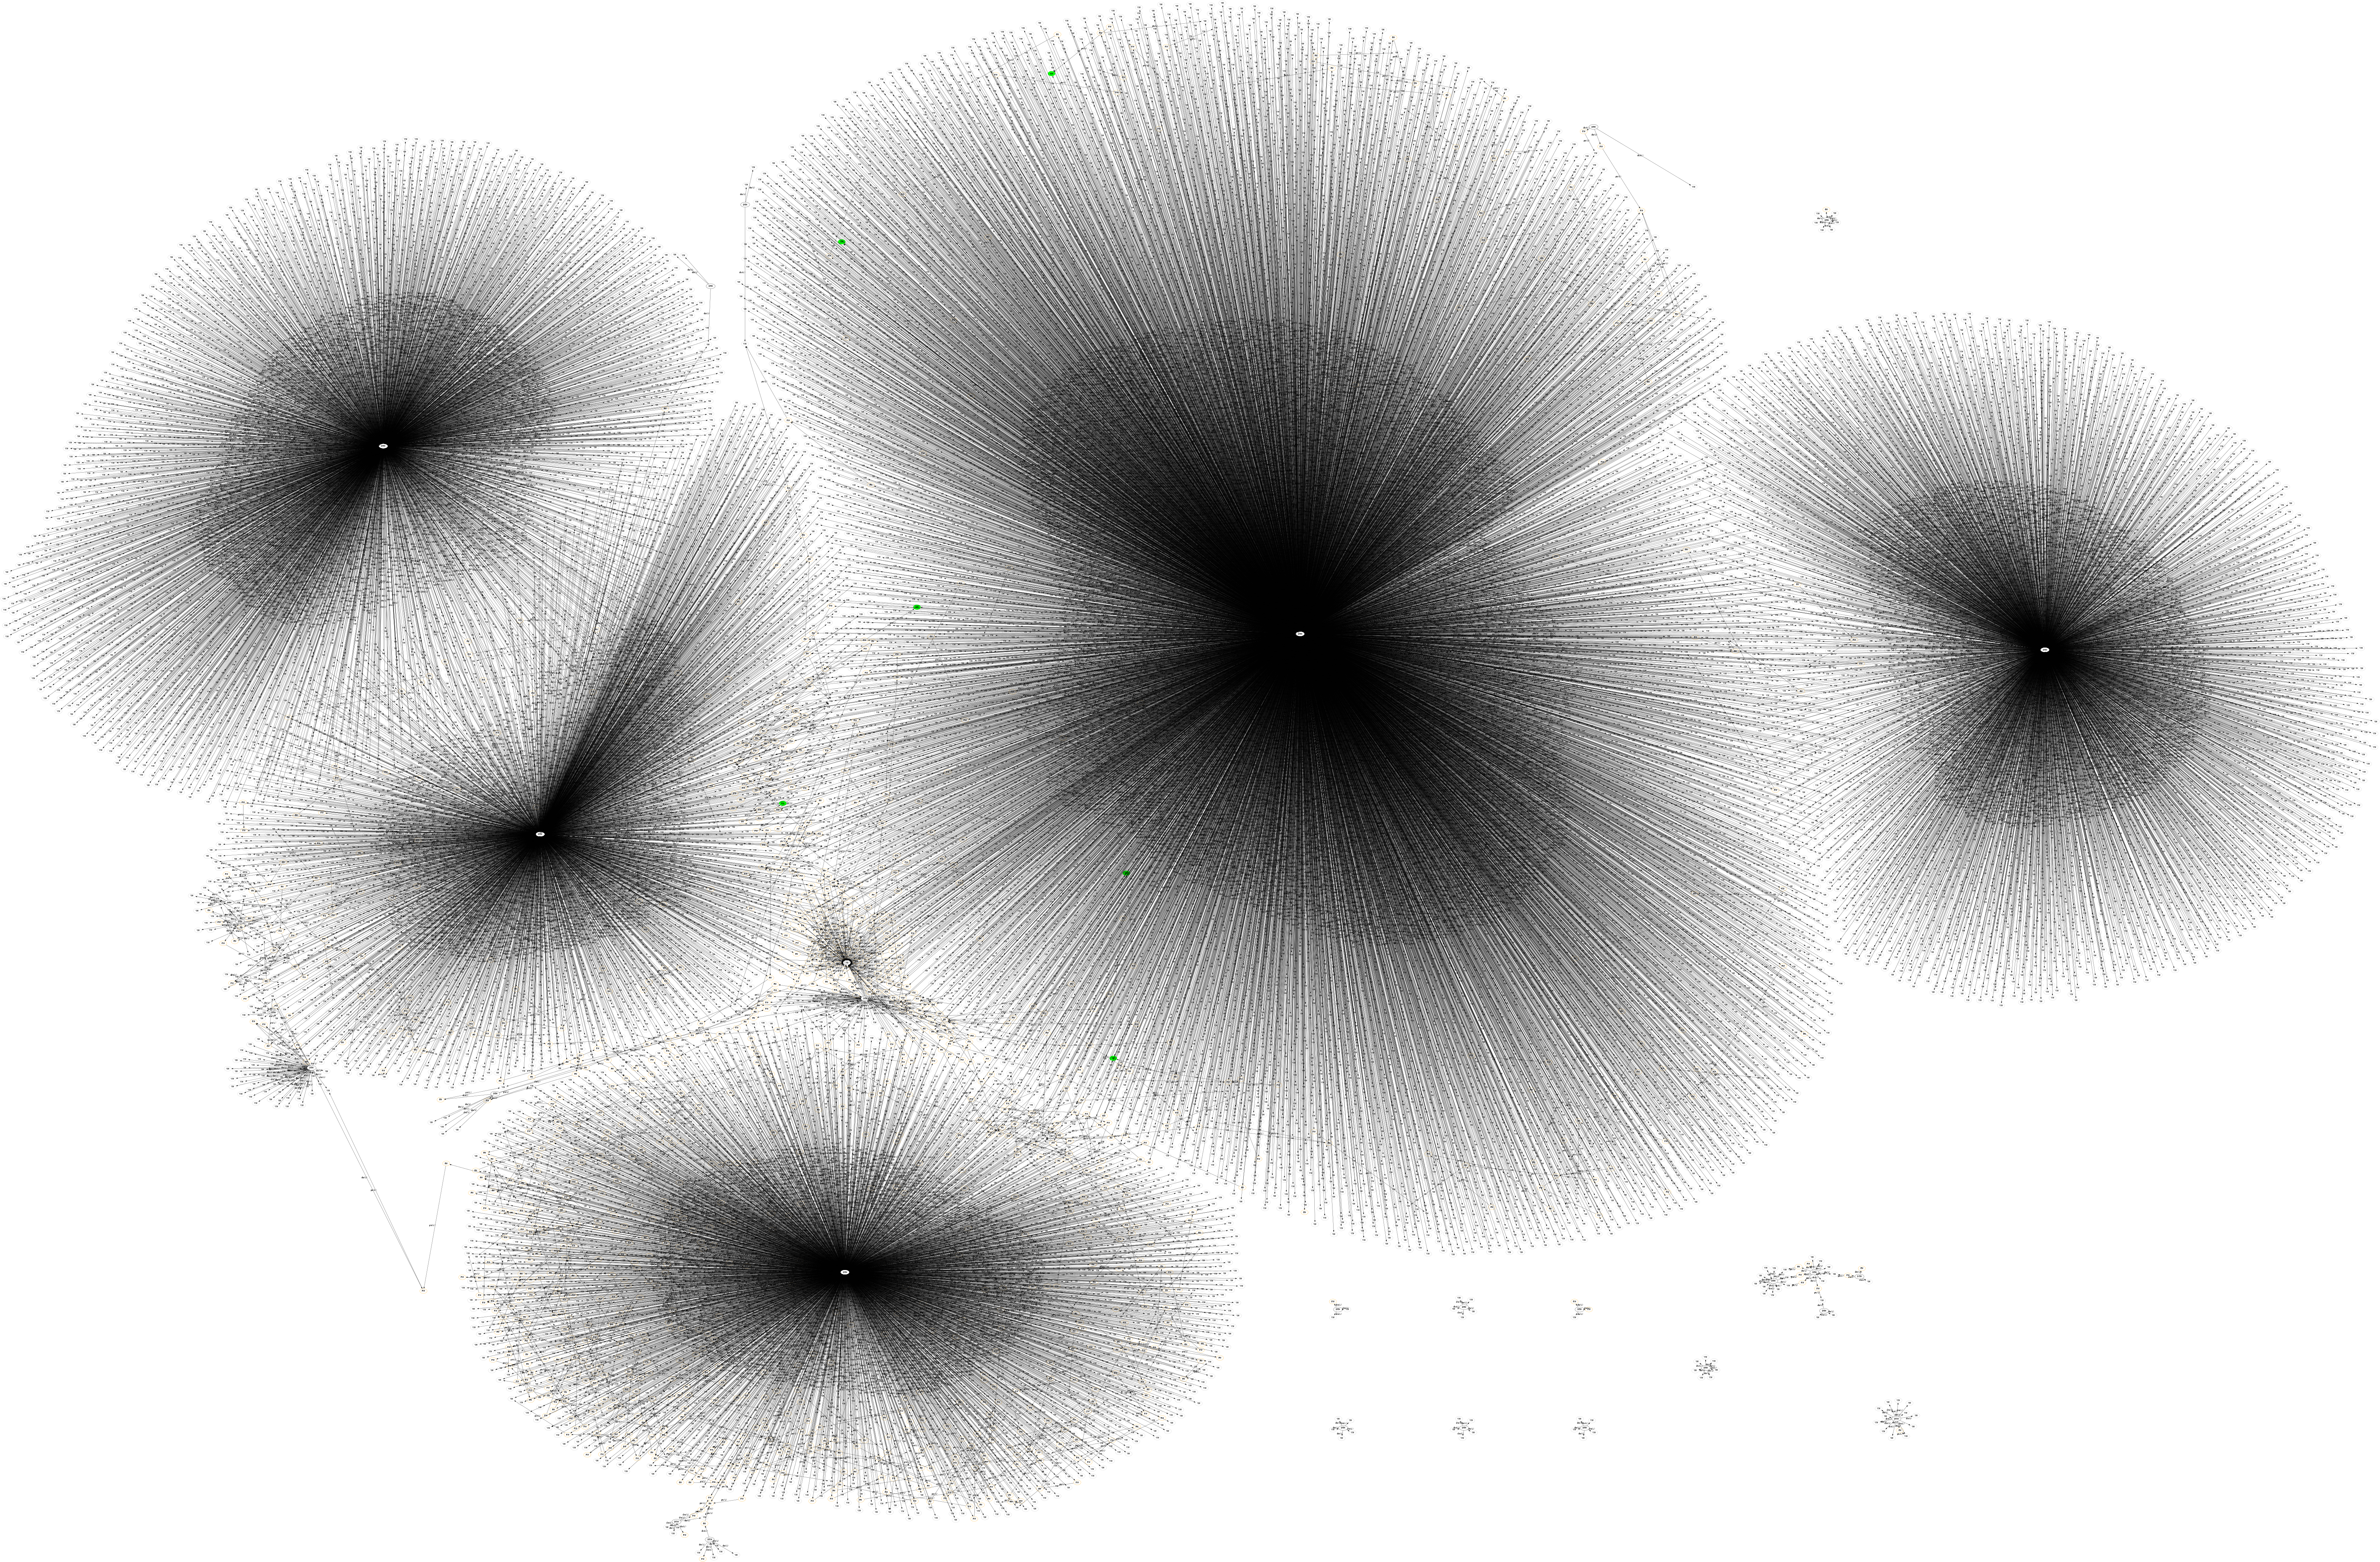
\includegraphics[width=16cm]{graphs/test_graph_from_302-1644391327_vn-sfdp.jpg}
    \caption{Visualization of the full memory graph generated from \textit{Training/scp/V\_7\_8\_P1/16/302-1644391327-heap.raw}.}
\end{figure}

\begin{figure}[H]\label{appendix:mem_graph:17016-1643962152:full}
    \centering
    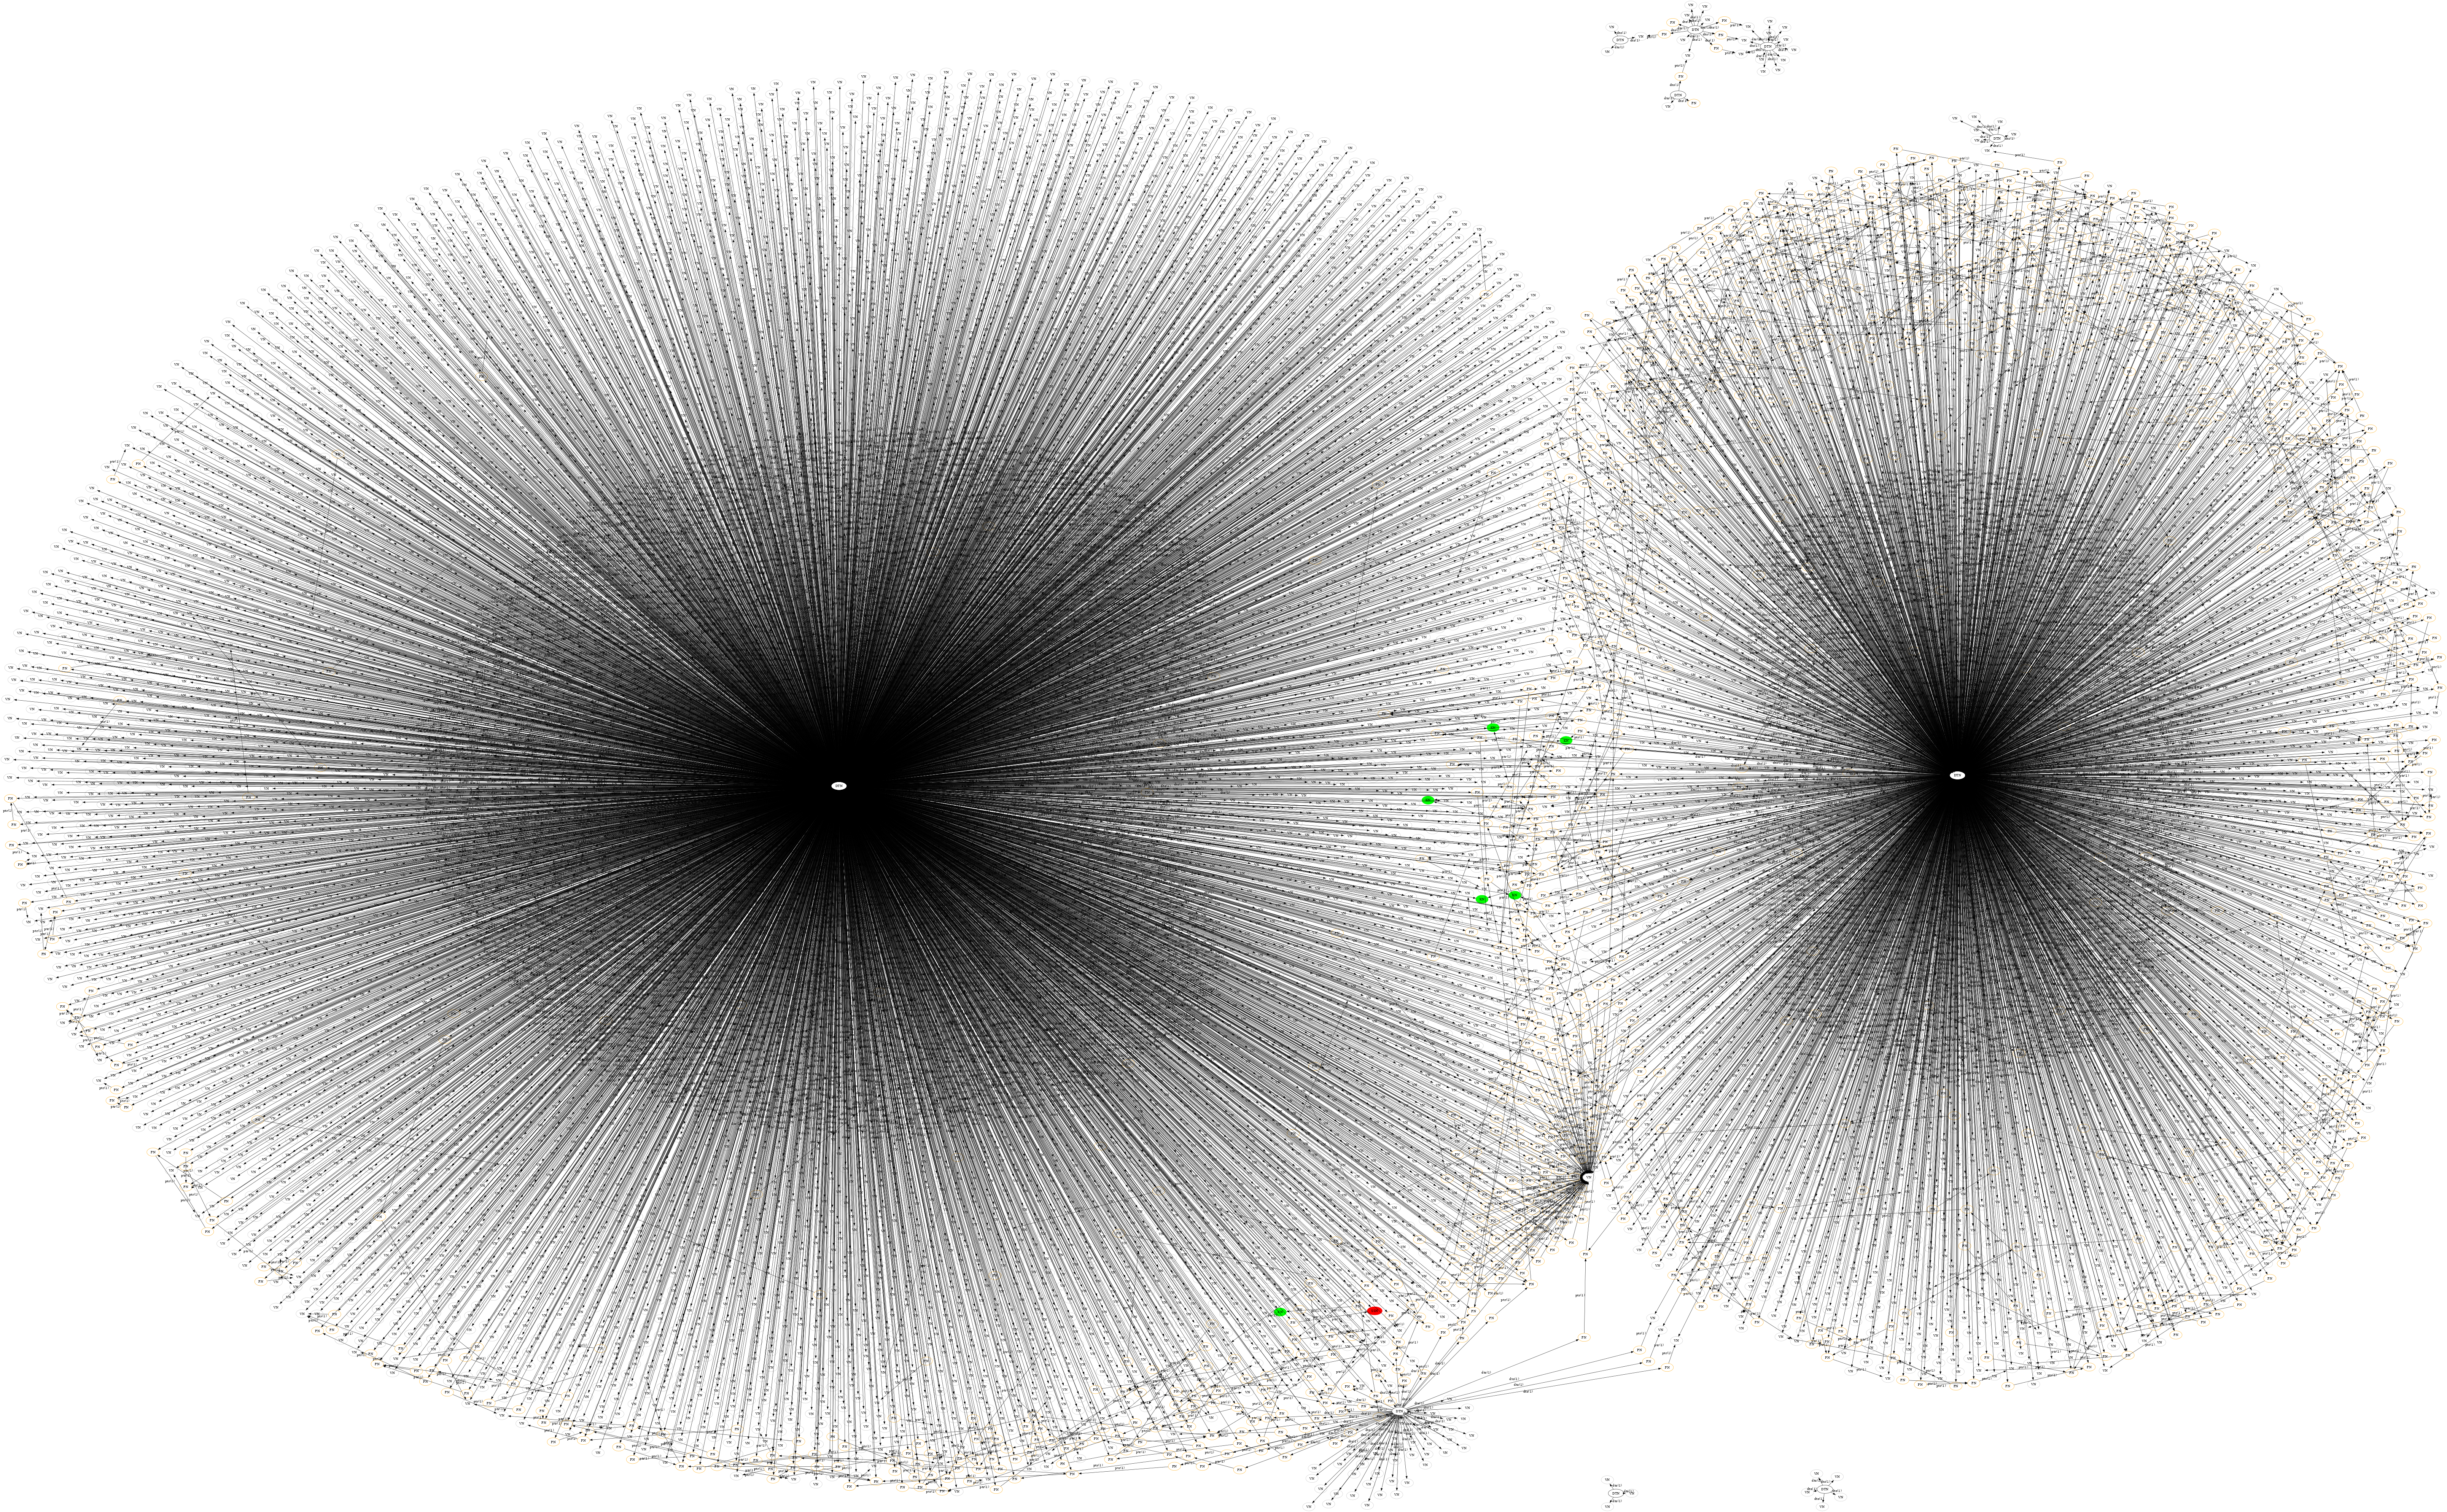
\includegraphics[width=16cm]{graphs/Training_basic_V_7_1_P1_24_17016-1643962152-heap.raw_dot_vn-sfdp.jpg}
    \caption{Visualization of the full memory graph generated from \textit{Training/basic/V\_7\_1\_P1/24/17016-1643962152-heap.raw}.}
\end{figure}

\begin{figure}[H]\label{appendix:mem_graph:17016-1643962152:truncated}
    \centering
    \includegraphics[width=16cm]{graphs/17016-1643962152_truncated.png}
    \caption{Visualization of a truncated memory graph generated from \textit{Training/basic/V\_7\_1\_P1/24/17016-1643962152-heap.raw}. Here with real addresses.}
\end{figure}

Generated using a slightly different command, for better layout of the nodes:

\begin{lstlisting}[language=bash, caption={Command used to generate the memory graph visualization of \textit{Training/basic/V\_7\_1\_P1/24/17016-1643962152-heap.raw} here using real addresses.}]
    sfdp -Gsize=30! -Goverlap=ortho -Tpng 17016-1643962152_truncated.gv > 17016-1643962152_truncated.png
\end{lstlisting}

\begin{figure}[H]
    \centering
    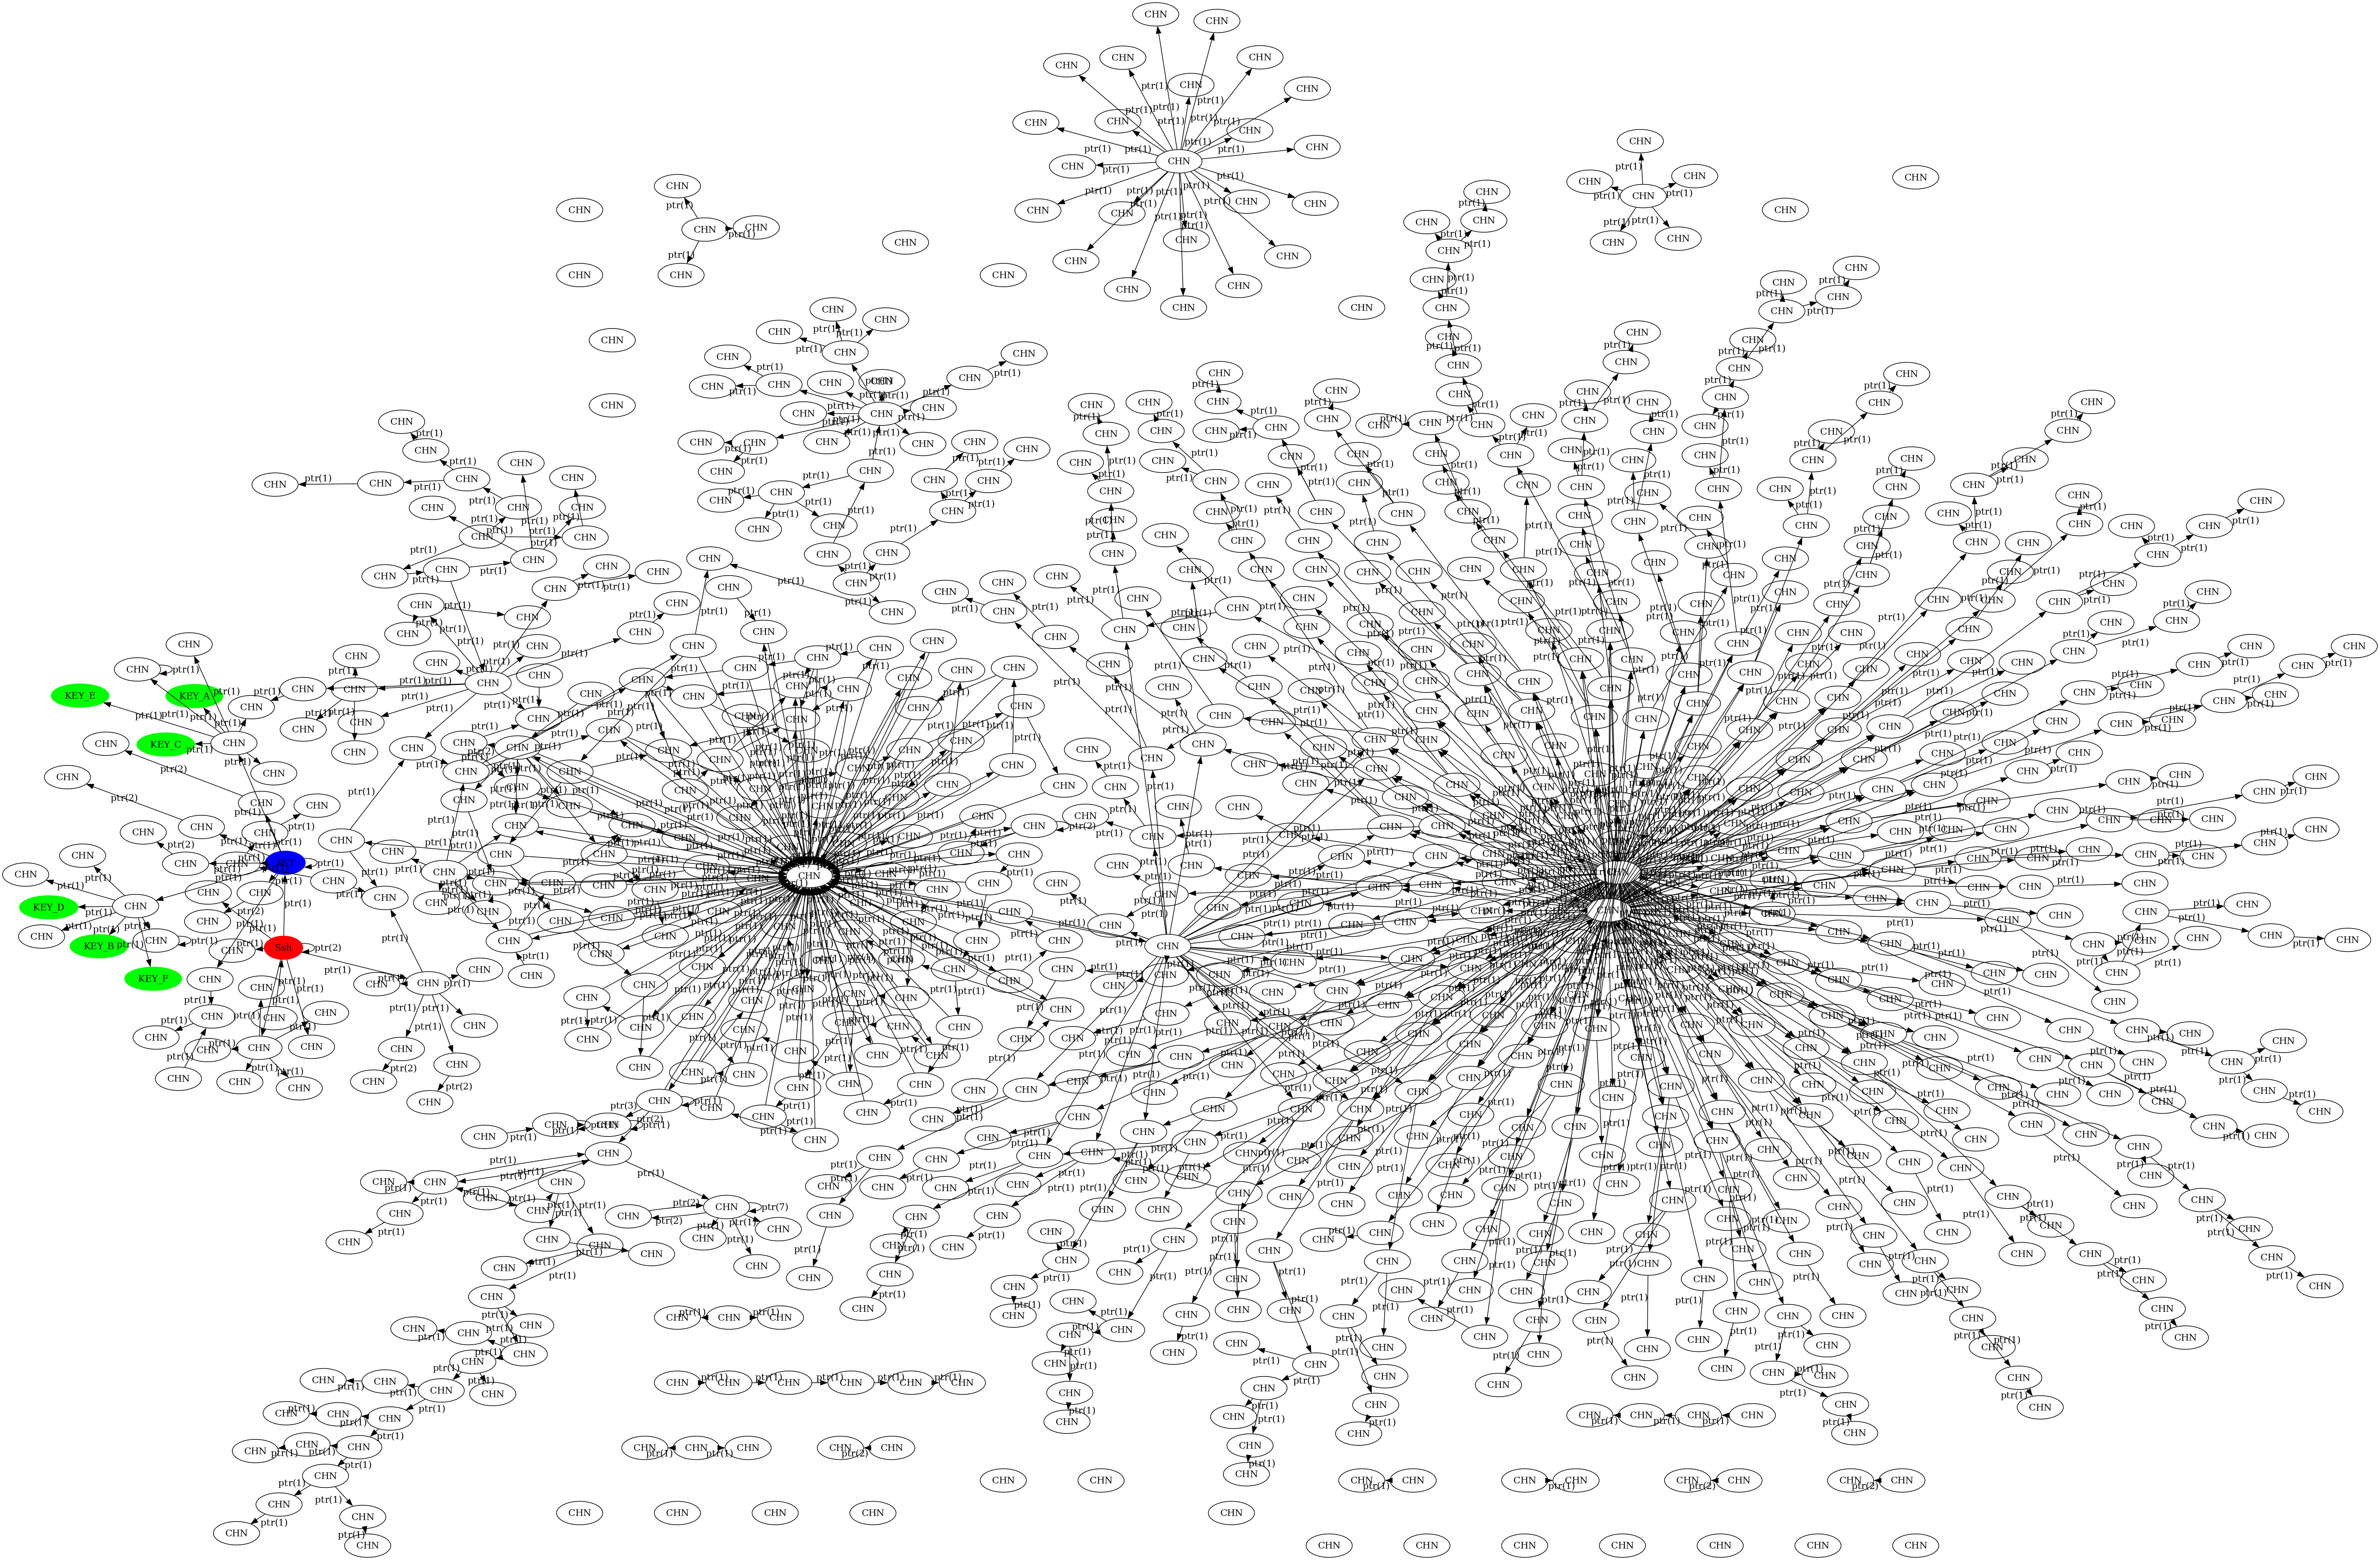
\includegraphics[width=16cm]{graphs/chunk_top_vn_semantic_home_onyr_code_phdtrack_phdtrack_data_clean_8708-1643979488-heap.raw_dot_no_vn_chn_annotation_no_vn-sfdp.png}
    \caption{Visualization of a chunk memory graph generated from \textit{Validation/Validation/basic/V\_7\_8\_P1/24/8708-1643979488-heap.raw}.}
\end{figure}

\begin{figure}[H]
    \centering
    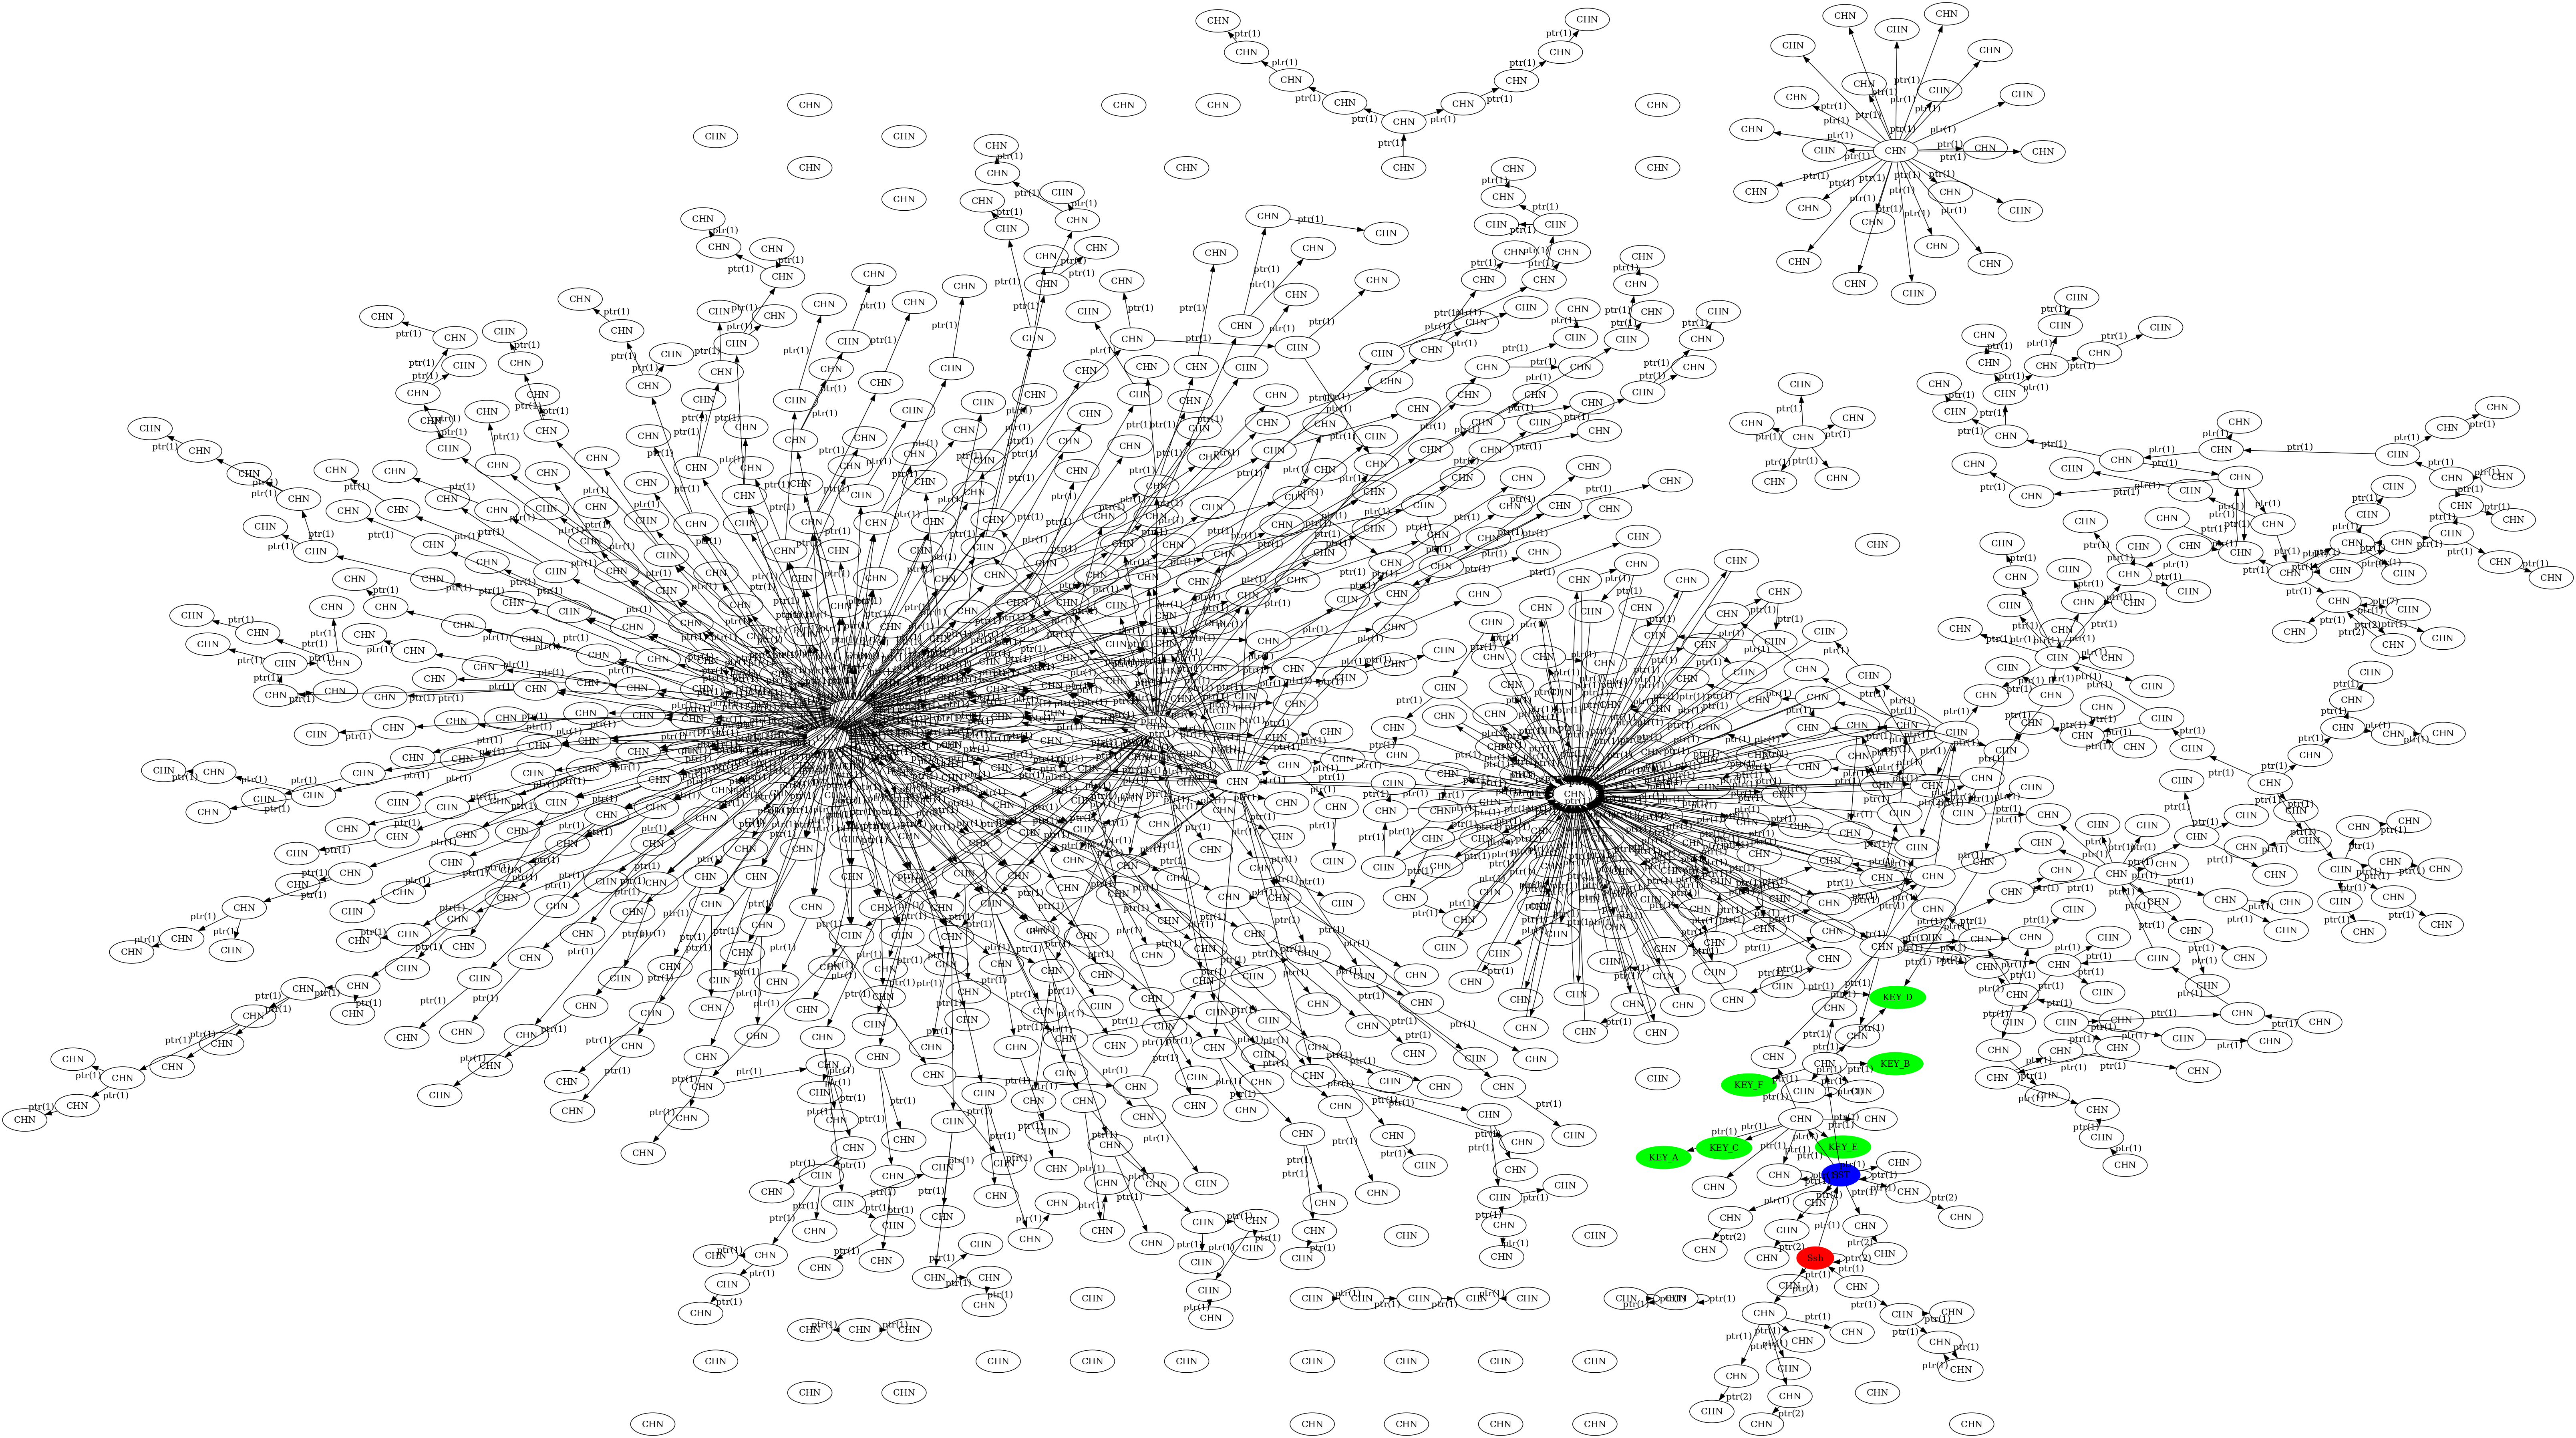
\includegraphics[width=16cm]{graphs/chunk_top_vn_semantic_home_onyr_code_phdtrack_phdtrack_data_clean_28621-1643890740-heap.raw_dot_no_vn_chn_annotation_no_vn-sfdp.png}
    \caption{Visualization of a chunk memory graph generated from \textit{Training/Training/basic/V\_6\_8\_P1/24/28621-1643890740-heap.raw}.}
\end{figure}

\section{Latest ML Experiment results}
The following are the latest results for ML experiments. Those tables were generated after the submission of the thesis.

\begin{table}[H]
    \centering
    \caption{Best instance for each model, with respect to accuracy.}
    \begin{tabular}{|l|c|c|c|c|c|c|} \hline 
      \textbf{Model}  & \textbf{Accuracy} & \textbf{Precision} & \textbf{Recall} & \textbf{F1 Score} & \textbf{Embedding}  \\ \hline 
        random-forest & 0.9984 & 1.0000 & 0.0833 & 0.1538 & chunk-start-bytes \\ \hline 
        sgd-classifier & 0.9984 & 0.6250 & 0.2083 & 0.3125 & node2vec \\ \hline 
        logistic-regression & 0.9983 & 1.0000 & 0.0417 & 0.0800 & node2vec \\ \hline 
        advanced-gcn & 0.9969 & 0.0000 & 0.0000 & 0.0000 & node2vec \\ \hline 
        gcn-with-dropout & 0.9969 & 0.0000 & 0.0000 & 0.0000 & node2vec \\ \hline 
        first-gcn & 0.9963 & 0.0000 & 0.0000 & 0.0000 & node2vec-chunk-statistic \\ \hline 
        simple-gcn & 0.9962 & 0.0000 & 0.0000 & 0.0000 & chunk-statistic \\ \hline 
        very-simple-gcn & 0.9959 & 0.0000 & 0.0000 & 0.0000 & node2vec \\ \hline 
    \end{tabular}
\end{table}


\begin{table}[H]
    \centering
    \caption{Best instance for each model, with respect to precision.}
    \begin{tabular}{|l|c|c|c|c|c|c|} \hline 
      \textbf{Model}  & \textbf{Accuracy} & \textbf{Precision} & \textbf{Recall} & \textbf{F1 Score} & \textbf{Embedding}  \\ \hline 
        logistic-regression & 0.9944 & 1.0000 & 0.0417 & 0.0800 & node2vec \\ \hline 
        random-forest & 0.9983 & 1.0000 & 0.0417 & 0.0800 & chunk-start-bytes \\ \hline 
        sgd-classifier & 0.9983 & 1.0000 & 0.0417 & 0.0800 & node2vec \\ \hline 
        very-simple-gcn & 0.9946 & 0.6000 & 0.5000 & 0.5455 & node2vec \\ \hline 
        first-gcn & 0.9935 & 0.5000 & 0.5000 & 0.5000 & node2vec \\ \hline 
        simple-gcn & 0.9935 & 0.5000 & 0.5000 & 0.5000 & node2vec \\ \hline 
        gcn-with-dropout & 0.9920 & 0.3500 & 0.2333 & 0.2800 & node2vec \\ \hline 
        advanced-gcn & 0.9898 & 0.2097 & 0.4333 & 0.2826 & node2vec \\ \hline 
    \end{tabular}
\end{table}


\begin{table}[H]
    \centering
    \caption{Best instance for each model, with respect to recall.}
    \begin{tabular}{|l|c|c|c|c|c|c|} \hline 
      \textbf{Model}  & \textbf{Accuracy} & \textbf{Precision} & \textbf{Recall} & \textbf{F1 Score} & \textbf{Embedding}  \\ \hline 
        first-gcn & 0.9826 & 0.2727 & 1.0000 & 0.4286 & node2vec \\ \hline 
        sgd-classifier & 0.9924 & 0.4615 & 1.0000 & 0.6316 & node2vec \\ \hline 
        simple-gcn & 0.9783 & 0.2308 & 1.0000 & 0.3750 & node2vec \\ \hline 
        very-simple-gcn & 0.9815 & 0.2609 & 1.0000 & 0.4138 & node2vec \\ \hline 
        advanced-gcn & 0.8887 & 0.0533 & 0.9000 & 0.1006 & node2vec \\ \hline 
        gcn-with-dropout & 0.9613 & 0.0863 & 0.8000 & 0.1558 & node2vec \\ \hline 
        logistic-regression & 0.9912 & 0.3333 & 0.5000 & 0.4000 & node2vec \\ \hline 
        random-forest & 0.9984 & 1.0000 & 0.0833 & 0.1538 & chunk-start-bytes \\ \hline 
    \end{tabular}
\end{table}


\begin{table}[H]
    \centering
    \caption{Best instance for each model, with respect to f1 score.}
    \begin{tabular}{|l|c|c|c|c|c|c|} \hline 
      \textbf{Model}  & \textbf{Accuracy} & \textbf{Precision} & \textbf{Recall} & \textbf{F1 Score} & \textbf{Embedding}  \\ \hline 
        sgd-classifier & 0.9924 & 0.4615 & 1.0000 & 0.6316 & node2vec \\ \hline 
        very-simple-gcn & 0.9946 & 0.6000 & 0.5000 & 0.5455 & node2vec \\ \hline 
        first-gcn & 0.9935 & 0.5000 & 0.5000 & 0.5000 & node2vec \\ \hline 
        simple-gcn & 0.9935 & 0.5000 & 0.5000 & 0.5000 & node2vec \\ \hline 
        logistic-regression & 0.9912 & 0.3333 & 0.5000 & 0.4000 & node2vec \\ \hline 
        gcn-with-dropout & 0.9858 & 0.2110 & 0.7667 & 0.3309 & node2vec \\ \hline 
        advanced-gcn & 0.9898 & 0.2097 & 0.4333 & 0.2826 & node2vec \\ \hline 
        random-forest & 0.9984 & 1.0000 & 0.0833 & 0.1538 & chunk-start-bytes \\ \hline 
    \end{tabular}
\end{table}


\begin{table}
    \centering
    \caption{Best model instance for each metric.}
    \begin{tabular}{|l|c|c|c|c|c|c|} \hline 
      \textbf{Metric} & \textbf{Model}  & \textbf{Accuracy} & \textbf{Precision} & \textbf{Recall} & \textbf{F1 Score} & \textbf{Embedding}  \\ \hline 
        accuracy & random-forest & 0.9984 & 1.0000 & 0.0833 & 0.1538 & chunk-start-bytes \\ \hline 
        precision & logistic-regression & 0.9944 & 1.0000 & 0.0417 & 0.0800 & node2vec \\ \hline 
        recall & first-gcn & 0.9826 & 0.2727 & 1.0000 & 0.4286 & node2vec \\ \hline 
        f1 score & sgd-classifier & 0.9924 & 0.4615 & 1.0000 & 0.6316 & node2vec \\ \hline 
    \end{tabular}
\end{table}


\end{appendices}

% glossary and acronyms
\newpage
% \printglossary[type=\acronymtype, title=Acronymes]
% \printglossary[title=Glossaire]
\printglossary[type=\acronymtype]

\printglossary

% biblio
\newpage
\printbibliography[
    heading=bibintoc,
    category=cited,
    title={References}
]

% uncited references (bibliography)
% https://tex.stackexchange.com/questions/6967/how-to-split-bibliography-into-works-cited-and-works-not-cited
\printbibliography[
    notcategory=cited,
    heading=bibintoc,
    title={Additional bibliography},
]

% -- Eidesstattliche Erklärung (= Affadavit)
\include{tex/eidesstattlicheErklaerung}

\restoregeometry
\end{document}